% Main file of the thesis, based on the PoliMi template for MSc theses
% (School of Industrial and Information Engineering, classical format).

\documentclass{Configuration_Files/PoliMi3i_thesis}

%------------------------------------------------------------------------------
%	REQUIRED PACKAGES AND CONFIGURATIONS
%------------------------------------------------------------------------------

% CONFIGURATIONS
\usepackage{parskip} % For paragraph layout
\usepackage{setspace} % For using single or double spacing
\usepackage{emptypage} % To insert empty pages
\usepackage{multicol} % To write in multiple columns (executive summary)
\setlength\columnsep{15pt} % Column separation in executive summary
\setlength\parindent{0pt} % Indentation
\raggedbottom

% PACKAGES FOR TITLES
\usepackage{titlesec}
\titlespacing{\section}{0pt}{3.3ex}{2ex}
\titlespacing{\subsection}{0pt}{3.3ex}{1.65ex}
\titlespacing{\subsubsection}{0pt}{3.3ex}{1ex}
\usepackage{color}

% PACKAGES FOR LANGUAGE AND FONT
\usepackage[english]{babel} % The document is in English
\usepackage[utf8]{inputenc} % UTF8 encoding
\usepackage[T1]{fontenc} % Font encoding
\usepackage[11pt]{moresize} % Big fonts

% PACKAGES FOR IMAGES
\usepackage{graphicx}
\usepackage{transparent} % Enables transparent images
\usepackage{eso-pic} % For the background picture on the title page
\usepackage{subfig} % Numbered and caption subfigures using \subfloat.
\usepackage{tikz} % A package for high-quality hand-made figures.
\usetikzlibrary{positioning,fit,arrows.meta,calc,shapes.geometric,decorations.pathreplacing}
\graphicspath{{./Images/}} % Directory of the template images
\usepackage{caption} % Coloured captions
\usepackage{xcolor} % Coloured captions
\usepackage{amsthm,thmtools,xcolor} % Coloured "Theorem"
\usepackage{float}

% STANDARD MATH PACKAGES
\usepackage{amsmath}
\usepackage{amsthm}
\usepackage{amssymb}
\usepackage{amsfonts}
\usepackage{bm}
\usepackage[overload]{empheq} % For braced-style systems of equations.
\usepackage{fix-cm} % To override original LaTeX restrictions on sizes

% PACKAGES FOR TABLES
\usepackage{tabularx}
\usepackage{longtable} % Tables that can span several pages
\usepackage{colortbl}

% PACKAGES FOR ALGORITHMS (PSEUDO-CODE)
\usepackage{algorithm}
\usepackage{algorithmic}

% PACKAGES FOR REFERENCES & BIBLIOGRAPHY
\usepackage[colorlinks=true,linkcolor=black,anchorcolor=black,citecolor=black,filecolor=black,menucolor=black,runcolor=black,urlcolor=black]{hyperref} % Adds clickable links at references
\usepackage{cleveref}
\usepackage[square, numbers, sort&compress]{natbib} % Square brackets, citing references with numbers, citations sorted by appearance in the text and compressed
\bibliographystyle{abbrvnat} % You may use a different style adapted to your field

% OTHER PACKAGES
\usepackage{pdfpages} % To include a pdf file
\usepackage{afterpage}
\usepackage{fancyhdr} % For the headers
\fancyhf{}

% Input of configuration file. Do not change config.tex file unless you really know what you are doing.
% Define blue color typical of polimi
\definecolor{bluepoli}{cmyk}{0.4,0.1,0,0.4}

% Custom theorem environments
\declaretheoremstyle[
  headfont=\color{bluepoli}\normalfont\bfseries,
  bodyfont=\color{black}\normalfont\itshape,
]{colored}

% Set-up caption colors
\captionsetup[figure]{labelfont={color=bluepoli}} % Set colour of the captions
\captionsetup[table]{labelfont={color=bluepoli}} % Set colour of the captions
\captionsetup[algorithm]{labelfont={color=bluepoli}} % Set colour of the captions

\theoremstyle{colored}
\newtheorem{theorem}{Theorem}[chapter]
\newtheorem{proposition}{Proposition}[chapter]

% Enhances the features of the standard "table" and "tabular" environments.
\newcommand\T{\rule{0pt}{2.6ex}}
\newcommand\B{\rule[-1.2ex]{0pt}{0pt}}

% Pseudo-code algorithm descriptions.
\newcounter{algsubstate}
\renewcommand{\thealgsubstate}{\alph{algsubstate}}
\newenvironment{algsubstates}
  {\setcounter{algsubstate}{0}%
   \renewcommand{\STATE}{%
     \stepcounter{algsubstate}%
     \Statex {\small\thealgsubstate:}\space}}
  {}

% New font size
\newcommand\numfontsize{\@setfontsize\Huge{200}{60}}

% Title format: chapter
\titleformat{\chapter}[hang]{
\fontsize{50}{20}\selectfont\bfseries\filright}{\textcolor{bluepoli} \thechapter\hsp\hspace{2mm}\textcolor{bluepoli}{|   }\hsp}{0pt}{\huge\bfseries \textcolor{bluepoli}
}

% Title format: section
\titleformat{\section}
{\color{bluepoli}\normalfont\Large\bfseries}
{\color{bluepoli}\thesection.}{1em}{}

% Title format: subsection
\titleformat{\subsection}
{\color{bluepoli}\normalfont\large\bfseries}
{\color{bluepoli}\thesubsection.}{1em}{}

% Title format: subsubsection
\titleformat{\subsubsection}
{\color{bluepoli}\normalfont\large\bfseries}
{\color{bluepoli}\thesubsubsection.}{1em}{}

% Shortening for setting no horizontal-spacing
\newcommand{\hsp}{\hspace{0pt}}

\makeatletter
% Renewcommand: cleardoublepage including the background pic
\renewcommand*\cleardoublepage{%
  \clearpage\if@twoside\ifodd\c@page\else
  \null
  \AddToShipoutPicture*{\BackgroundPic}
  \thispagestyle{empty}%
  \newpage
  \if@twocolumn\hbox{}\newpage\fi\fi\fi}
\makeatother

%For correctly numbering algorithms
\numberwithin{algorithm}{chapter}

%----------------------------------------------------------------------------
%	ADD YOUR PACKAGES (be careful of package interaction)
%----------------------------------------------------------------------------
\usepackage{array,booktabs,siunitx}
\usepackage{xurl}

%----------------------------------------------------------------------------
%	ADD YOUR DEFINITIONS AND COMMANDS (be careful of existing commands)
%----------------------------------------------------------------------------
% Macros used by the chapters. \input this file in the preamble of the thesis.
% Requires: xcolor, graphicx, array, booktabs, siunitx, amsmath
\newcommand{\TODO}[1]{\textcolor{red}{[TODO: #1]}}
\newcommand{\figplaceholder}[3]{\fbox{\parbox[c][#2][c]{#1}{\centering\small #3}}}
\usepackage{placeins}   % \FloatBarrier
\usepackage{float}     % [H] placement


%----------------------------------------------------------------------------
%	BEGIN OF YOUR DOCUMENT
%----------------------------------------------------------------------------

\begin{document}

\fancypagestyle{plain}{%
\fancyhf{} % Clear all header and footer fields
\fancyhead[RO,RE]{\thepage} %RO=right odd, RE=right even
\renewcommand{\headrulewidth}{0pt}
\renewcommand{\footrulewidth}{0pt}}

%----------------------------------------------------------------------------
%	TITLE PAGE (to be added)
%----------------------------------------------------------------------------

\pagestyle{empty} % No page numbers
\frontmatter % Use roman page numbering style (i, ii, iii, iv...) for the preamble pages

% \puttitle{
% 	title=Title, % Title of the thesis
% 	name=Name Surname, % Author Name and Surname
% 	course=Xxxxxxx Engineering - Ingegneria Xxxxxxx, % Study Programme (in Italian)
% 	ID  = 000000,  % Student ID number (numero di matricola)
% 	advisor= Prof. Name Surname, % Supervisor name
% 	coadvisor={Name Surname, Name Surname}, % Co-Supervisor name, remove this line if there is none
% 	academicyear={20XX-XX},  % Academic Year
% }

%----------------------------------------------------------------------------
%	PREAMBLE PAGES: ABSTRACT (inglese e italiano)
%----------------------------------------------------------------------------
\startpreamble
\setcounter{page}{1} % Set page counter to 1

% ABSTRACT IN ENGLISH
\chapter*{Abstract}
\TODO{}
\\
\\
\textbf{Keywords:} \TODO{}

% ABSTRACT IN ITALIAN
\chapter*{Abstract in lingua italiana}
\TODO{}
\\
\\
\textbf{Parole chiave:} \TODO{}

%----------------------------------------------------------------------------
%	TABLE OF CONTENTS
%----------------------------------------------------------------------------
\thispagestyle{empty}
\tableofcontents
\thispagestyle{empty}
\cleardoublepage

%-------------------------------------------------------------------------
%	THESIS MAIN TEXT
%-------------------------------------------------------------------------
\addtocontents{toc}{\vspace{2em}} % Add a gap in the Contents, for aesthetics
\mainmatter % Begin numeric (1,2,3...) page numbering

\chapter{Introduction}
\label{ch:intro}

\TODO{}

% =====================================================================
%  Chapter 2 - Experimental Setup and Methodology
% =====================================================================

\chapter{Experimental Setup and Methodology}
\label{ch:setup}

This chapter gives an overview of the hardware and software setup of the fully
autonomous racecars on which this research is based. The work considers two different
vehicles: the Dallara AV-24, which competes in the Indy Autonomous Challenge (IAC), and
the Dallara EAV-25, which competes in the Abu Dhabi Autonomous Racing League (A2RL). Both
cars are equipped with the sensors and the software stack used to design, run and
evaluate the algorithms presented in the following chapters.

Section~\ref{sec:operating_conditions} gives an overview of the two championships.
Section~\ref{sec:av24} and Section~\ref{sec:eav24} introduce the
two racecars together with their sensors. Section~\ref{sec:sensors} presents the working principle of the
exteroceptive sensors (LiDARs, RaDARs and cameras) used for opponent tracking and the
units mounted on the two vehicles. Finally,
Section~\ref{sec:sw_arch} gives an overview of the main modules of the software
architecture.

% =====================================================================
\section{Autonomous Racing Competitions}
\label{sec:operating_conditions}

This section gives an overview of the competitions in which the vehicles described in
this chapter take part.

\paragraph{Indy Autonomous Challenge.} The IAC started in 2019 with a series of simulation
challenges and held its first event on track in 2021, at the Indianapolis Motor Speedway.
All the teams race with the same vehicle provided by the organisers. Historically, the events have been held mainly on oval tracks, such as the
Indianapolis Motor Speedway, the Las Vegas Motor Speedway, during the Consumer Electronics
Show, and the Texas Motor Speedway. Since
2023 the series has also raced on road courses, starting from Monza, and in the last two
seasons it has raced at WeatherTech Raceway Laguna Seca (Fig.~\ref{fig:av24}), where in
2026 it held its first head-to-head competition on a road course.

\begin{figure}[H]
    \centering
    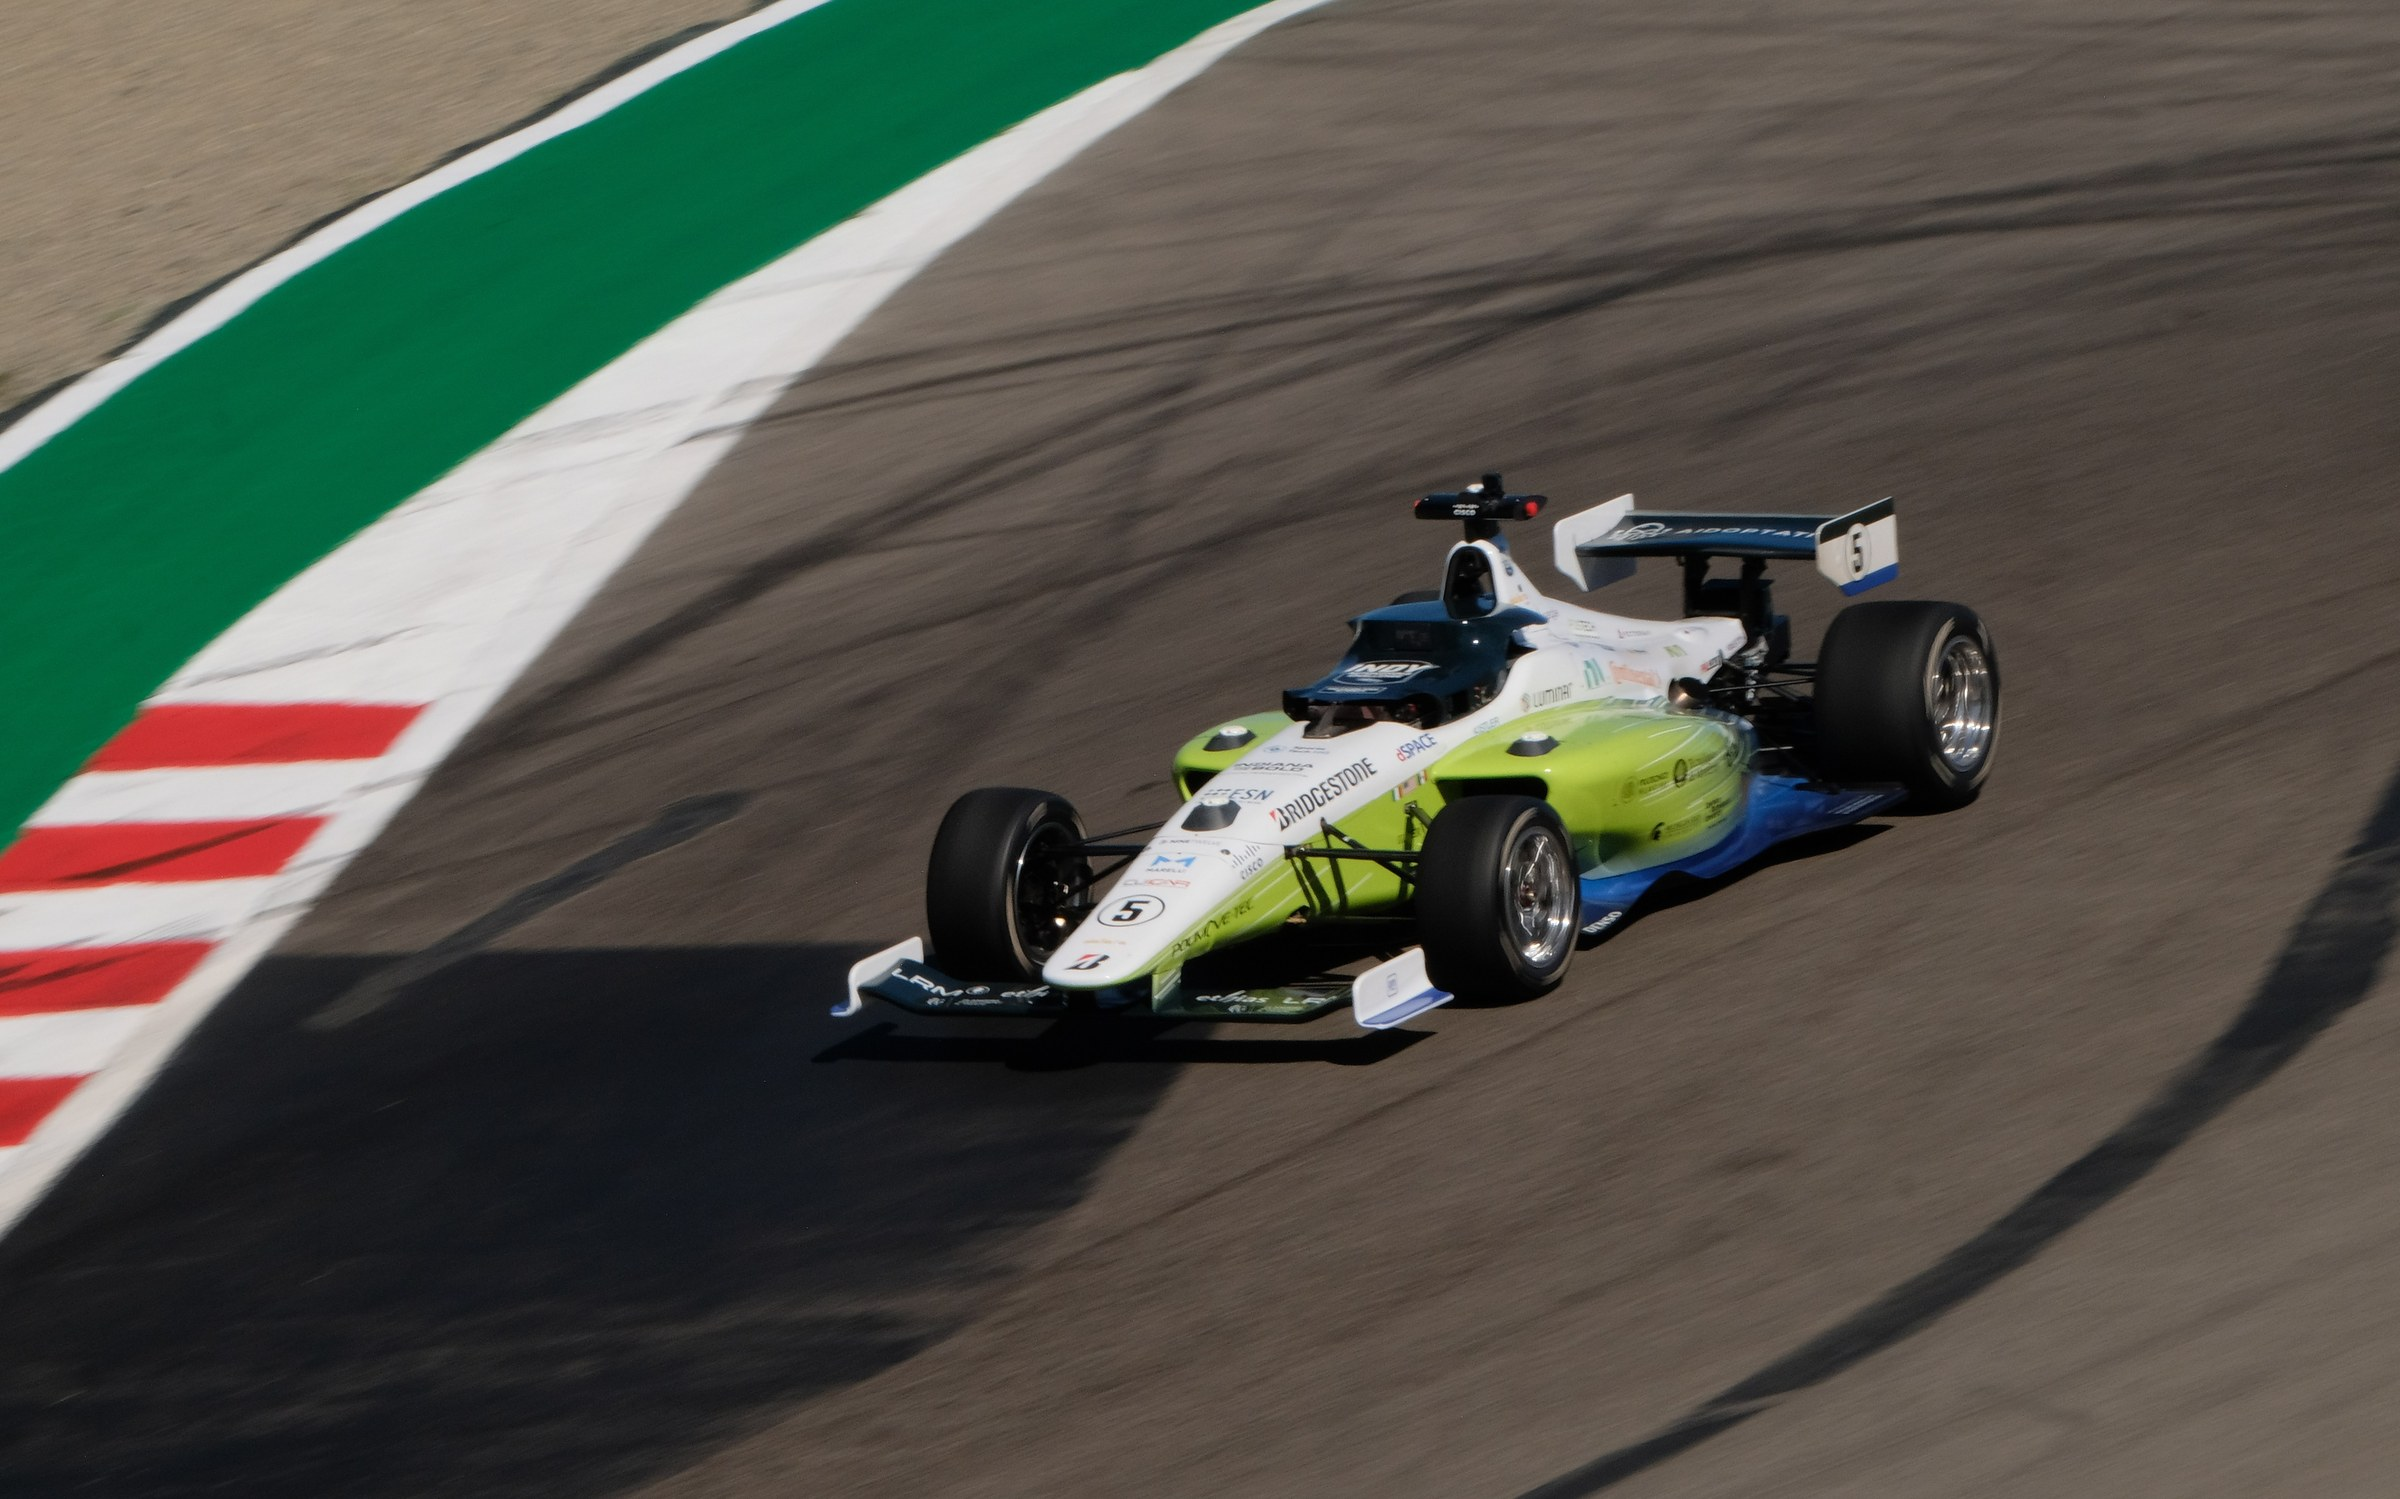
\includegraphics[width=0.85\textwidth]{figures/ch2/av24_laguna_seca.jpg}
    \caption{Dallara AV-24 at Laguna Seca, August 2026.}
    \label{fig:av24}
\end{figure}

\paragraph{Abu Dhabi Autonomous Racing League.} The A2RL is organised by ASPIRE, part of
the Advanced Technology Research Council of Abu Dhabi, and debuted in April 2024 at the
Yas Marina Circuit, with a race between four autonomous cars. Unlike the IAC, it was
conceived from the beginning for road circuits, with a larger number of corners and a
continuous alternation of braking, cornering and acceleration phases. In September 2026
it raced at the Autodromo Internazionale Enzo e Dino Ferrari in Imola, with five cars on
track (Fig.~\ref{fig:eav24}).

\begin{figure}[H]
    \centering
    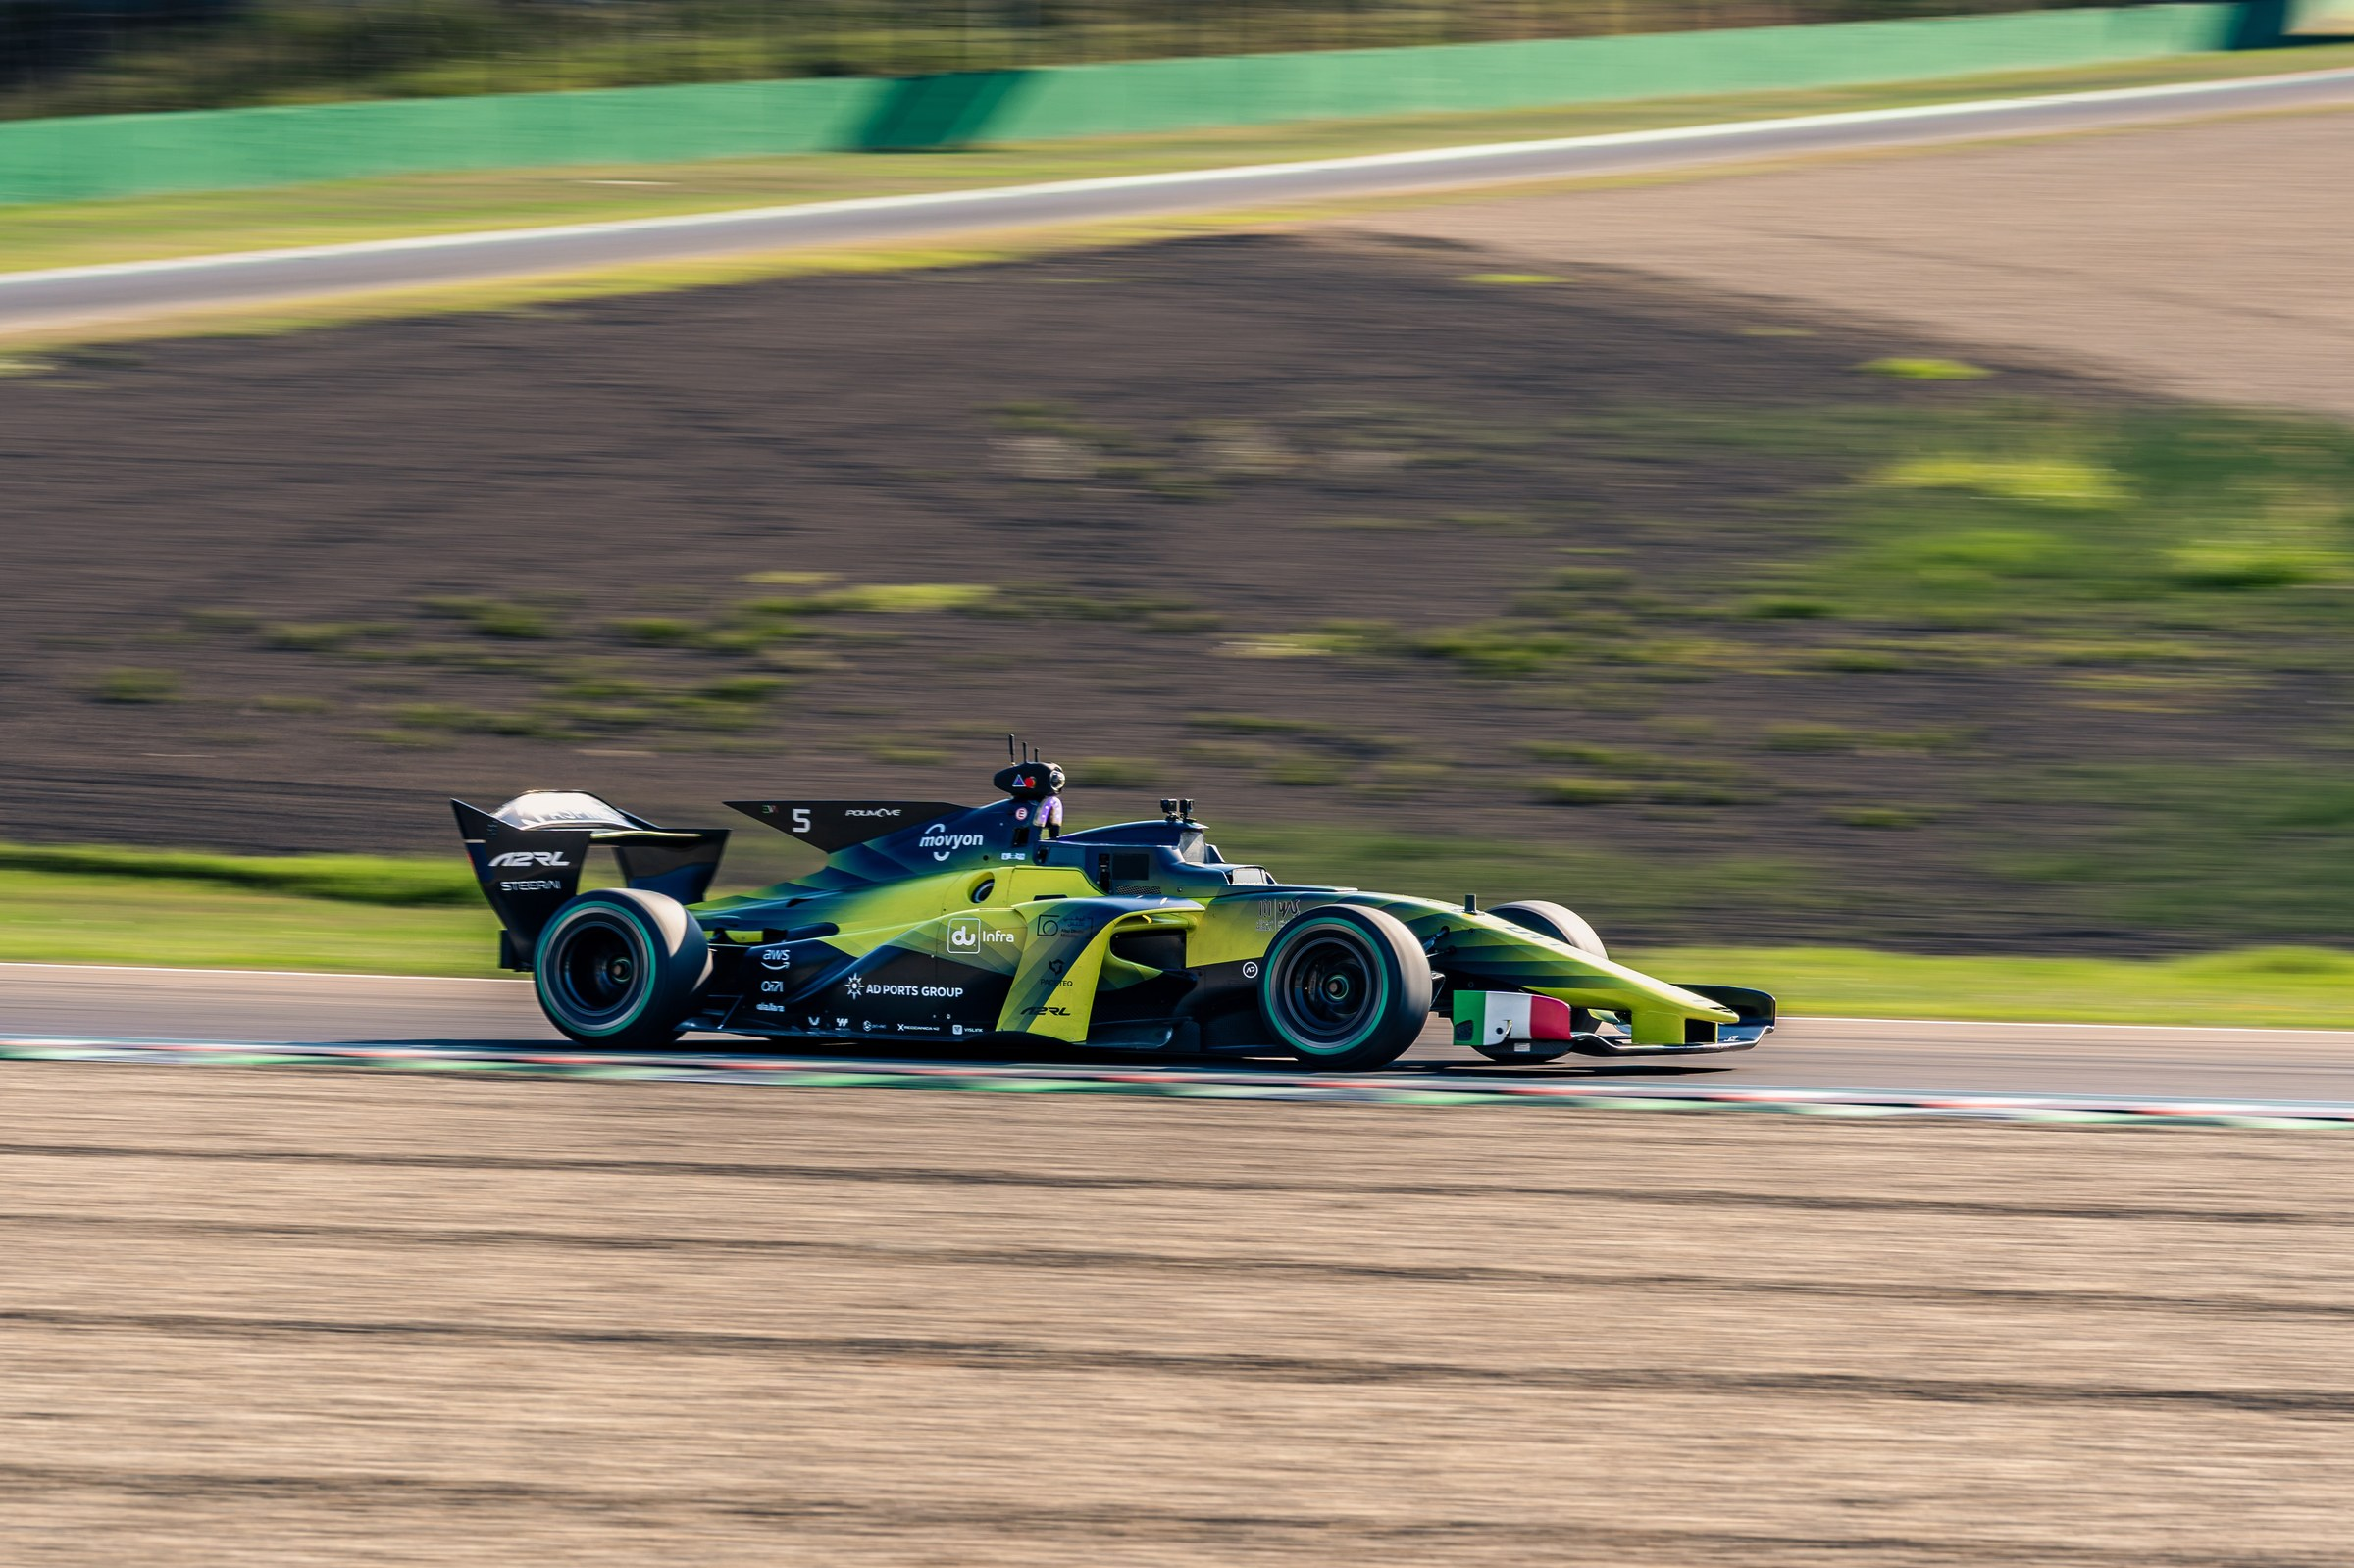
\includegraphics[width=0.85\textwidth]{figures/ch2/eav24_imola.jpg}
    \caption{Dallara EAV-25 at Imola circuit, August 2026.}
    \label{fig:eav24}
\end{figure}

\paragraph{Formats.} Both championships include single-vehicle and multi-target formats.
In single-vehicle formats, such as time trials and qualifying, each car is alone on track
and is ranked on its fastest lap: the focus is entirely on driving the vehicle
autonomously at the limits of its dynamic capabilities. In multi-target formats, instead,
the vehicle shares the track with other cars. In the IAC, the passing competition tests
the interaction between two vehicles in a head-to-head elimination bracket, in which an
attacking car tries to overtake a defending one. In the A2RL, the qualifying is followed
by the race, in which several cars race together on the same track.

Overall, in both competitions the vehicles are pushed to the limits of their dynamic
performance, reaching speeds above \SI{250}{km/h} and high lateral accelerations. This represents an extremely fertile context in which to
test the capabilities of autonomous driving.

\FloatBarrier

% =====================================================================
\section{Dallara AV-24}
\label{sec:av24}

The Dallara AV-24 (Fig.~\ref{fig:av24}) is the official vehicle of the IAC and the
second generation of racecars adopted by the series, introduced in 2024 as the successor
of the AV-21. It is built by Dallara on the chassis of the Indy NXT, the open-wheel
single-seater of the development series of IndyCar, and has been adapted to driverless
operation while keeping the layout and the performance of the original car. The
vehicle has been designed to compete on oval tracks.

To enable autonomous operation, the cockpit hosts the on-board computer and the set of
actuators that turns the commands of the control software into steering, throttle,
brake and gear inputs to the vehicle, together with the power and network distribution
that connects sensors, computer and actuators. The bodywork has been modified to carry
the sensors, and a radio link connects the
car to the base station, which receives the telemetry and sends the race control
signals. The main characteristics of the vehicle are collected in
Table~\ref{tab:av24}.


\begin{table}[H]
    \centering
    \small
    \begin{tabular}{p{0.3\textwidth}p{0.45\textwidth}}
        \toprule
        Item              & Specification \\
        \midrule
        Series            & Indy Autonomous Challenge (IAC) \\
        Engine            & 4 Piston Racing K20C, \SI{2.0}{l} turbocharged four-cylinder \\
        Power             & \SI{488}{hp} \\
        Gearbox           & Ricardo, six-speed sequential \\
        Top speed         & over \SI{300}{km/h} \\
        Mass              & \SI{748}{kg} \\
        Length / width / height & \SI{4.88}{m} / \SI{1.93}{m} / \SI{1.16}{m} \\
        \bottomrule
    \end{tabular}
    \caption{Main characteristics of the Dallara AV-24.}
    \label{tab:av24}
\end{table}

To enable autonomous driving, the vehicle has been equipped with a set of sensors that
are heterogeneous in some aspects and redundant in others: the
LiDARs provide a dense and accurate description of the shape of the surrounding objects,
the RaDARs measure directly the relative velocity and reach longer distances, and the
cameras provide rich images from which the vehicles can be recognized reliably. Each type
of sensor has its own strengths and limitations, and their combination enables a full
perception of the surroundings, accurate and robust in all the operating conditions and
over the dynamics and the distances of interest. On the AV-24, the perception of the
surroundings relies on three LiDARs, two RaDARs and six cameras, described in
Section~\ref{sec:sensors}, while the state of the ego vehicle is estimated from a
VectorNav VN-310 GNSS/INS and two NovAtel PwrPak7 receivers, which provide position,
attitude, velocity and acceleration with centimetre-level position accuracy.


\FloatBarrier

% =====================================================================
\section{Dallara EAV-25}
\label{sec:eav24}

The Dallara EAV-25 (Fig.~\ref{fig:eav24}) is the official vehicle of the A2RL. It is
developed from the Dallara SF23, the single-seater of the Japanese Super Formula
championship, and keeps its chassis and aerodynamic package.

Unlike the AV-24, the EAV-25 is conceived for road circuits; therefore, the vehicle is
designed for high performance in heavy braking, in slow and fast corners and, in
general, in more challenging dynamical conditions. The power unit is a turbocharged
\SI{2.0}{l} four-cylinder engine delivering about \SI{450}{hp}, which can be raised
temporarily to about \SI{550}{hp} with the push-to-pass, coupled with a
longitudinal six-speed sequential gearbox, which brings the car to a top speed of about
\SI{300}{km/h}.

As on the AV-24, the cockpit hosts the on-board computer and the actuation system that
executes the commands of the control software, and the bodywork carries the sensors.
The main characteristics are summarized in
Table~\ref{tab:eav24}.


\begin{table}[H]
    \centering
    \small
    \begin{tabular}{p{0.3\textwidth}p{0.45\textwidth}}
        \toprule
        Item              & Specification \\
        \midrule
        Series            & Abu Dhabi Autonomous Racing League (A2RL) \\
        Engine            & 4 Piston Racing K20C1, \SI{2.0}{l} turbocharged four-cylinder \\
        Power             & \SI{450}{hp} (\SI{550}{hp} with push-to-pass) \\
        Gearbox           & 3MO, six-speed sequential \\
        Top speed         & about \SI{300}{km/h} \\
        Mass              & \SI{742}{kg} \\
        Length / width / height & \SI{5.24}{m} / \SI{1.93}{m} / \SI{0.97}{m} \\
        \bottomrule
    \end{tabular}
    \caption{Main characteristics of the Dallara EAV-25.}
    \label{tab:eav24}
\end{table}

As on the AV-24, the vehicle has been equipped with a set of heterogeneous and redundant
sensors to enable autonomous driving. On the EAV-25, the perception of the surroundings
relies on three LiDARs, four RaDARs and seven cameras, described in
Section~\ref{sec:sensors}, while the state of the ego vehicle is estimated from a
dual-antenna VectorNav VN-310 RTK-GNSS/INS, which includes an inertial measurement unit,
and from a Kistler SF~Motion optical sensor, which measures the longitudinal and lateral
ground speed of the vehicle.


\FloatBarrier

% =====================================================================
\section{Sensors}
\label{sec:sensors}

This section describes the sensors mounted on the Dallara AV-24 and EAV-25. For each type
of sensor, the working principle and its main strengths and limitations are presented
first; then, the description goes into the details of the specific set of sensors mounted
on each vehicle.

% ---------------------------------------------------------------------
\subsection{LiDAR}
\label{subsec:lidar}

A LiDAR (Light Detection and Ranging) is an active sensor that emits laser pulses and
measures the distance of the surfaces that reflect them from the time of flight of each
pulse, $r = c\,\Delta t/2$. A scanning mechanism steers the beam in azimuth and
elevation, and the high pulse repetition rate allows hundreds of thousands of points to
be acquired every second. The output of each scan is a point cloud: a dense
three-dimensional sampling of the surrounding surfaces, with centimetre-level range
precision and an angular resolution of a few hundredths of a degree. From the point cloud
the shape and the size of the objects around the vehicle can be reconstructed.

Due to the nature of its working principle, the quality of the measurements degrades in
adverse weather, since rain, fog and the spray raised by other cars attenuate and
scatter the laser beam. Moreover, the energy returned by a target decreases quickly
with the distance and with the reflectivity of its surface, so that the working range
is shorter than that of RaDAR technologies. Finally, a LiDAR measures positions only:
the velocity of a target is not observed directly and has to be inferred from
successive scans.

\subsubsection{Dallara AV-24}

The AV-24 mounts three Luminar Iris LiDARs: one at the front of the cockpit, facing
forward, and two on the sides of the cockpit, oriented at $\pm\SI{112.5}{\degree}$
with respect to the longitudinal axis. The Iris operates at a wavelength of \SI{1550}{nm}
with a dual-scanning optical system, which sweeps the field of view at 640 lines per
second: the number of scan lines in each frame therefore depends on the frame rate, and
at the \SI{10}{Hz} used in the application each frame contains 64 lines. The vertical
field of view, up to \SI{26}{\degree}, and the distribution of the scan lines within it
can be configured in real time, choosing between uniform scan patterns, in which the lines
are evenly spaced, and non-uniform ones, for instance Gaussian, which concentrate the
lines around the horizon, where the opponents are expected. The main characteristics of the sensor are reported in
Table~\ref{tab:lidar_av24}.

\begin{table}[H]
    \centering
    \footnotesize
    \begin{tabular}{>{\raggedright\arraybackslash}p{0.35\textwidth}>{\raggedright\arraybackslash}p{0.35\textwidth}}
        \toprule
        Model                             & Luminar Iris \\
        Units                             & 3 \\
        Wavelength                        & \SI{1550}{nm} \\
        FoV (H $\times$ V)                & \SI{120}{\degree} $\times$ \SI{26}{\degree} (configurable) \\
        Angular resolution (H $\times$ V) & \SI{0.12}{\degree} $\times$ \SI{0.05}{\degree} \\
        Scan lines                        & 640 lines/s \\
        Maximum range                     & \SI{200}{m} (10\% reflectivity) \\
        Range precision                   & ${<}\SI{2}{cm}$ (\SI{50}{m}) \\
        Update rate                       & \SI{10}{Hz} \\
        \bottomrule
    \end{tabular}
    \caption{Main characteristics of the LiDARs mounted on the Dallara AV-24.}
    \label{tab:lidar_av24}
\end{table}

Each unit covers \SI{120}{\degree} in azimuth, so that the three LiDARs together cover
the horizontal plane around the vehicle, except for a narrow sector behind it
(Fig.~\ref{fig:av24_lidar_fov}). To give an idea of the density of the point cloud,
consider for example an opponent with the dimensions of the AV-24 reported in
Table~\ref{tab:av24}, i.e.\ \SI{1.93}{m} wide and \SI{1.16}{m} high, \SI{50}{m} straight
ahead of the sensor and seen from behind: it covers an angle of
about \SI{2.2}{\degree} in the horizontal direction and \SI{1.3}{\degree} in the vertical
one. With a horizontal resolution of \SI{0.12}{\degree}, each scan line returns about 18
points on its rear. In the vertical direction, with a uniform pattern over
\SI{26}{\degree} the 64 lines are about \SI{0.4}{\degree} apart, and the opponent is
crossed by about 3 lines, for a total of about 55 points per frame; with a pattern that
concentrates the lines around the horizon, the number of lines on the opponent, and thus
of points, increases accordingly. The number of points is range related, i.e.\ it
decreases with the range.

\begin{figure}[H]
    \centering
    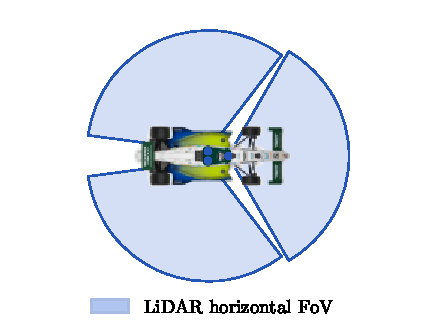
\includegraphics[width=0.6\textwidth]{figures/ch2/av24_lidar_fov.pdf}
    \caption{Horizontal field of view of the LiDARs of the Dallara AV-24. The radius of
    the sectors is not to scale, and the occlusion caused by the rear wing is not
    represented.}
    \label{fig:av24_lidar_fov}
\end{figure}

The nominal performance reported in Table~\ref{tab:lidar_av24} is obtained in ideal
working conditions and for targets of known reflectivity. In the application, the
opponent is far from an ideal target, mainly because of the limited reflectivity of its
bodywork, and the data show that the effective detection range is limited to about
80--\SI{100}{m}; beyond this distance, the detections become fewer and sparser. In
addition, the rear wing of the ego vehicle occludes the field of view of the LiDARs
towards the back of the car and creates a proper blind spot, whose effect becomes more
and more evident as the opponent aligns with the longitudinal axis of the ego vehicle.

\subsubsection{Dallara EAV-25}

The EAV-25 is equipped with three Innovusion Falcon Kinetic LiDARs: one at the front of
the cockpit, facing forward, and two on the sides of the cockpit, oriented at
$\pm\SI{120}{\degree}$ with respect to the longitudinal axis. The Falcon Kinetic is a
semi-solid-state LiDAR, also operating at \SI{1550}{nm}, which scans up to 1500 lines
per second and is used at \SI{10}{Hz}. Its angular resolution is
\SI{0.18}{\degree} $\times$ \SI{0.24}{\degree} and can be increased to
\SI{0.09}{\degree} $\times$ \SI{0.08}{\degree} in a specific region of interest of
\SI{40}{\degree} $\times$ \SI{4.8}{\degree}, whose position within the field of view can be
configured in real time; in this way, the density of points can be increased where the
opponents are expected, for instance around the horizon in front of the car. The main
characteristics of the sensor are reported in
Table~\ref{tab:lidar_eav24}.

\begin{table}[H]
    \centering
    \footnotesize
    \begin{tabular}{>{\raggedright\arraybackslash}p{0.35\textwidth}>{\raggedright\arraybackslash}p{0.35\textwidth}}
        \toprule
        Model                             & Innovusion Falcon Kinetic \\
        Units                             & 3 \\
        Wavelength                        & \SI{1550}{nm} \\
        FoV (H $\times$ V)                & \SI{120}{\degree} $\times$ \SI{25}{\degree} \\
        Angular resolution (H $\times$ V) & \SI{0.18}{\degree} $\times$ \SI{0.24}{\degree} \\
        Angular resolution in the region of interest (H $\times$ V) & \SI{0.09}{\degree} $\times$ \SI{0.08}{\degree} (\SI{40}{\degree} $\times$ \SI{4.8}{\degree}) \\
        Scan lines                        & up to 1500 lines/s \\
        Maximum range                     & \SI{250}{m} (10\% reflectivity) \\
        Update rate                       & \SI{10}{Hz} \\
        \bottomrule
    \end{tabular}
    \caption{Main characteristics of the LiDARs mounted on the Dallara EAV-25.}
    \label{tab:lidar_eav24}
\end{table}

In the same example made for the AV-24, an opponent with the dimensions of the EAV-25
reported in Table~\ref{tab:eav24}, i.e.\ \SI{1.93}{m} wide and \SI{0.97}{m} high,
\SI{50}{m} straight ahead and seen from behind, covers about
\SI{2.2}{\degree} $\times$ \SI{1.1}{\degree}. Outside the region of interest, it is sampled
by about 12 points on each scan line and by 4--5 lines, i.e.\ about 55 points per frame;
inside the region of interest, by about 24 points on each of about 14 lines, i.e.\ more
than 300 points. The three
LiDARs, oriented at \SI{120}{\degree} from each other, nominally cover the whole
horizontal plane (Fig.~\ref{fig:eav24_lidar_fov}).

\begin{figure}[H]
    \centering
    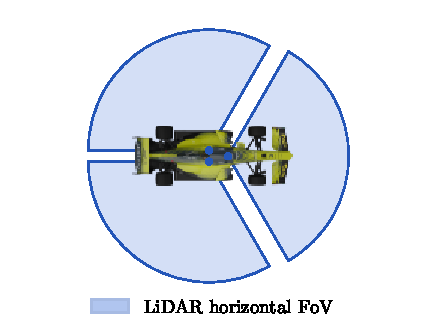
\includegraphics[width=0.6\textwidth]{figures/ch2/eav24_lidar_fov.pdf}
    \caption{Horizontal field of view of the LiDARs of the Dallara EAV-25. The radius of
    the sectors is not to scale, and the occlusion caused by the rear wing is not
    represented.}
    \label{fig:eav24_lidar_fov}
\end{figure}

The same considerations made for the AV-24 on the effective range and on the blind spot
caused by the rear wing apply.

% ---------------------------------------------------------------------
\subsection{RaDAR}
\label{subsec:radar}

A RaDAR (Radio Detection and Ranging) is an active sensor that emits electromagnetic
waves in the radio band and receives the echoes reflected by the targets. Automotive
RaDARs are typically frequency-modulated continuous-wave (FMCW) sensors: the
transmitted signal is a sequence of frequency ramps, and the frequency difference
between the transmitted and the received signal is proportional to the range of the
target. The direction of the target is obtained from the phase differences of the echo
across the receiving antennas.

The main strength of the RaDAR is the direct measurement of velocity. When the target
moves with respect to the sensor, the phase of its echo changes from one ramp to the
next by an amount proportional to the radial component of the relative velocity
(Doppler effect):
\begin{equation}
    \Delta\varphi = \frac{4\pi}{\lambda}\,\dot\rho\,T_c
    \quad\Longrightarrow\quad
    \dot\rho = \frac{\lambda\,\Delta\varphi}{4\pi\,T_c},
    \label{eq:doppler}
\end{equation}
where $\lambda$ is the wavelength of the carrier, $T_c$ the time between two consecutive
ramps and $\Delta\varphi$ the phase difference of the echo between them; equivalently,
the echo is shifted in frequency by $|f_D| = 2|\dot\rho|/\lambda$ (Doppler shift). The
RaDAR therefore measures the \emph{range rate} $\dot\rho$, the rate of change of the
distance between the two vehicles, within a single scan.
The second strength is the range: radio waves are much less attenuated than light, so
the RaDAR detects a vehicle at larger distances than the LiDAR and extends the distance
at which an opponent is visible. For the same reason, it is also much less sensitive to
adverse weather, and its operation is guaranteed both during day and night.

The quality of the position measurement, on the other hand, is lower than that of the
LiDAR. The RaDAR does not reconstruct the three-dimensional shape of the target: the
echoes come from a few points on the most reflective parts of the vehicle. In addition,
the angular resolution is considerably coarser than that of LiDARs and cameras.

\subsubsection{Dallara AV-24}

The RaDAR coverage of the AV-24 is provided by two units of different models: a
Continental ARS548~RDI, mounted above the cockpit and facing forward, and a ZF FRGen21,
mounted at the rear of the car and facing backward. Both are \SI{77}{GHz} imaging RaDARs,
which return for each reflection point its range, azimuth, elevation and range rate.
Their main characteristics are reported in Table~\ref{tab:radar_av24}.

\begin{table}[H]
    \centering
    \footnotesize
    \setlength{\tabcolsep}{4pt}
    \begin{tabular}{>{\raggedright\arraybackslash}p{0.3\textwidth}>{\raggedright\arraybackslash}p{0.28\textwidth}>{\raggedright\arraybackslash}p{0.3\textwidth}}
        \toprule
                                          & Front RaDAR                      & Rear RaDAR \\
        \midrule
        Model                             & Continental ARS548 RDI           & ZF FRGen21 \\
        FoV (H $\times$ V)                & \SI{100}{\degree} $\times$ \SI{28}{\degree} (${<}\SI{100}{m}$) & \SI{90}{\degree} $\times$ \SI{30}{\degree} (\SI{150}{m}) \\
        Angular resolution (H $\times$ V) & 1.2--\SI{1.68}{\degree} $\times$ \SI{2.3}{\degree} & \SI{1.5}{\degree} $\times$ \SI{1.5}{\degree} \\
        Maximum range                     & \SI{300}{m}                      & \SI{95}{m} / \SI{190}{m} / \SI{350}{m} \\
        Range resolution                  & \SI{0.22}{m}                     & \SI{0.21}{m} / \SI{0.41}{m} / \SI{0.77}{m} \\
        Relative speed range              & $-111$ to $+\SI{56}{m/s}$        & -- \\
        Range rate resolution             & \SI{0.1}{m/s}                    & \SI{0.1}{m/s} \\
        Update rate                       & \SI{20}{Hz}                      & \SI{16.7}{Hz} \\
        \bottomrule
    \end{tabular}
    \caption{Main characteristics of the RaDARs mounted on the Dallara AV-24.}
    \label{tab:radar_av24}
\end{table}

The ARS548~RDI detects targets up to \SI{300}{m}, within $\pm\SI{50}{\degree}$ in azimuth,
measures relative speeds between $-\SI{111}{m/s}$ (approaching targets) and
$+\SI{56}{m/s}$, and covers its whole field of view in a cycle time of about
\SI{50}{ms}, i.e.\ at \SI{20}{Hz}. For the FRGen21 the range mode can be selected: the
available modes go from a shorter to a longer range operation, and the range resolution
decreases as the maximum range increases. It covers $\pm\SI{45}{\degree}$ in azimuth up to
\SI{150}{m} and works at \SI{16.7}{Hz}. The RaDAR coverage is limited to two sectors, in
front of and behind the car (Fig.~\ref{fig:av24_radar_fov}): on the sides of the vehicle,
the opponent is observed only by the LiDARs and by the cameras, while behind it the rear
RaDAR covers the blind spot of the LiDARs.

\begin{figure}[H]
    \centering
    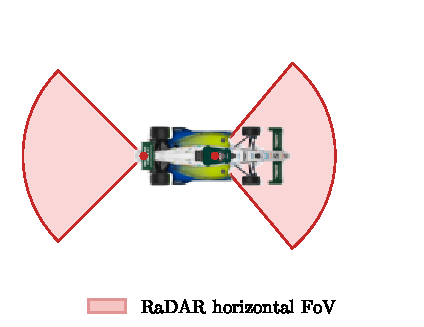
\includegraphics[width=0.6\textwidth]{figures/ch2/av24_radar_fov.pdf}
    \caption{Horizontal field of view of the RaDARs of the Dallara AV-24. The radius of the
    sectors is not to scale.}
    \label{fig:av24_radar_fov}
\end{figure}

In our case scenario, the effective range is also more limited than the nominal one, and
the RaDAR measures the opponent consistently up to about \SI{150}{m}. The echoes come
from a few reflective parts of the opponent, such as the wheels, the wings and the
metallic components: since the measured position depends on the reflectivity of the
target, it is related to the surface that the opponent exposes to the sensor, and
therefore to the relative geometry between the two vehicles, and it changes from one scan
to the next. Moreover, the walls, the bridges and the fences along the track are strong
reflectors, which generate echoes close to the opponent.

\subsubsection{Dallara EAV-25}

The EAV-25 mounts four ZF FRGen21 RaDARs, the same model mounted at the rear of the AV-24,
placed at the front, on the two sides and at the rear of the car. The sensor operates in
the 76--\SI{77}{GHz} band and measures range, azimuth, elevation and range rate of each
reflection point, with a fixed cycle time of \SI{60}{ms}, i.e.\ at \SI{16.7}{Hz}. As
described for the AV-24, the range mode can be selected among shorter and longer range
operation, with a range resolution that decreases as the maximum range increases. Its
main characteristics are
reported in Table~\ref{tab:radar_eav24}.

\begin{table}[H]
    \centering
    \footnotesize
    \begin{tabular}{>{\raggedright\arraybackslash}p{0.35\textwidth}>{\raggedright\arraybackslash}p{0.4\textwidth}}
        \toprule
        Model                             & ZF FRGen21 \\
        Units                             & 4 \\
        FoV (H $\times$ V)                & \SI{120}{\degree} (\SI{80}{m}), \SI{90}{\degree} (\SI{150}{m}) $\times$ \SI{30}{\degree} \\
        Angular resolution (H $\times$ V) & \SI{1.5}{\degree} $\times$ \SI{1.5}{\degree} \\
        Maximum range                     & \SI{95}{m} / \SI{190}{m} / \SI{350}{m} \\
        Range resolution                  & \SI{0.21}{m} / \SI{0.41}{m} / \SI{0.77}{m} \\
        Range rate resolution             & \SI{0.1}{m/s} \\
        Update rate                       & \SI{16.7}{Hz} \\
        \bottomrule
    \end{tabular}
    \caption{Main characteristics of the RaDARs mounted on the Dallara EAV-25.}
    \label{tab:radar_eav24}
\end{table}

The horizontal field of view reported in Table~\ref{tab:radar_eav24} is the nominal one of
each unit. In the application, the region of interest of each RaDAR is limited to
$\pm\SI{45}{\degree}$ around its boresight, so that the four sectors do not overlap and
together cover the whole horizontal plane around the vehicle
(Fig.~\ref{fig:eav24_radar_fov}). This choice also allows the blind spot of the LiDARs
behind the car to be recovered efficiently by the rear RaDAR.

\begin{figure}[H]
    \centering
    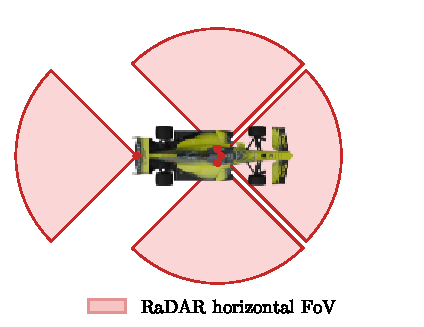
\includegraphics[width=0.6\textwidth]{figures/ch2/eav24_radar_fov.pdf}
    \caption{Horizontal field of view of the RaDARs of the Dallara EAV-25. The radius of the
    sectors is not to scale.}
    \label{fig:eav24_radar_fov}
\end{figure}

The same considerations made for the AV-24 on the effective range, on the reflection
points and on the echoes of the walls, bridges and fences apply.

% ---------------------------------------------------------------------
\subsection{Cameras}
\label{subsec:camera}

Cameras are passive sensors that capture images of the scene at high resolution and
frame rate. Their main strength is the semantic content of the images: colour, texture
and shape allow neural networks to detect and classify the surrounding objects reliably,
and for each vehicle in the field of view the detector returns a bounding box in the
image. The three-dimensional position of the vehicle is then reconstructed from the
bounding box, with the knowledge of the calibration of the cameras.

On the other hand, cameras are strongly affected by the environmental conditions. Being
passive sensors, they depend on the ambient light, so that the quality of the images
changes with the brightness of the scene, as well as with the weather. Moreover, the
depth is not measured directly but reconstructed indirectly from the image, and its
accuracy degrades as the distance of the target increases.

\subsubsection{Dallara AV-24}

Six Allied Vision Mako G319C cameras are arranged as a front stereo pair, two side
cameras oriented at $\pm\SI{100}{\degree}$ with respect to the longitudinal axis, and two
cameras on the roll hoop facing forward and backward, so that together they cover the
surroundings of the vehicle in every direction. The Mako G319C is based on the Sony IMX265
global-shutter sensor, with a resolution of about 3.2 megapixels at up to \SI{37.6}{fps}.
Its main characteristics are reported in Table~\ref{tab:cam_av24}.

\begin{table}[H]
    \centering
    \footnotesize
    \begin{tabular}{>{\raggedright\arraybackslash}p{0.3\textwidth}>{\raggedright\arraybackslash}p{0.55\textwidth}}
        \toprule
        Model              & Allied Vision Mako G319C \\
        Units              & 6 \\
        Image sensor       & Sony IMX265 \\
        Resolution         & $2064 \times 1544$ pixels \\
        Maximum frame rate & \SI{37.6}{fps} \\
        Arrangement        & front stereo pair (baseline \SI{0.36}{m}), two side cameras at $\pm\SI{100}{\degree}$, two roll hoop cameras (forward and backward) \\
        \bottomrule
    \end{tabular}
    \caption{Main characteristics of the cameras mounted on the Dallara AV-24.}
    \label{tab:cam_av24}
\end{table}

\subsubsection{Dallara EAV-25}

Seven Leopard Imaging cameras are arranged as a front stereo pair, two cameras facing the
sides of the vehicle and three cameras covering the region behind it, two on the roll
hoop and one at the rear end of the car, so that together they cover the surroundings of
the vehicle in every direction. They are based on the Sony IMX728 automotive sensor, with a
resolution of about 8.4 megapixels and high dynamic range, at up to \SI{45}{fps}. Their
main characteristics are reported in Table~\ref{tab:cam_eav24}.

\begin{table}[H]
    \centering
    \footnotesize
    \begin{tabular}{>{\raggedright\arraybackslash}p{0.3\textwidth}>{\raggedright\arraybackslash}p{0.55\textwidth}}
        \toprule
        Model              & Leopard Imaging \\
        Units              & 7 \\
        Image sensor       & Sony IMX728 \\
        Resolution         & $3857 \times 2177$ pixels \\
        Maximum frame rate & \SI{45}{fps} \\
        Arrangement        & front stereo pair (baseline \SI{0.32}{m}), two side cameras, three rear cameras (two on the roll hoop, one at the rear end) \\
        \bottomrule
    \end{tabular}
    \caption{Main characteristics of the cameras mounted on the Dallara EAV-25.}
    \label{tab:cam_eav24}
\end{table}

\FloatBarrier

% =====================================================================
\section{Software Architecture}
\label{sec:sw_arch}

The autonomous driving software, shared by the two vehicles, is organized in four
main modules: estimation, perception, planning and control (Fig.~\ref{fig:sw_arch}).
Each module runs continuously and exchanges data with the others, so that the
information flows from the sensors to the actuators through a chain in which the
output of one module is the input of the next.

\begin{figure}[H]
    \centering
    % Block diagram of the autonomous driving software (Section 2.4).
\begin{tikzpicture}[
    font=\footnotesize,
    >={Stealth[length=2mm]},
    blk/.style={draw, rounded corners=2pt, align=center, minimum height=8mm, inner sep=3pt},
    sens/.style={blk, minimum width=17mm, fill=gray!8},
    mod/.style={blk, minimum width=21mm, fill=blue!6},
    hl/.style={blk, minimum width=21mm, fill=blue!18, very thick},
    grp/.style={draw, dashed, rounded corners=4pt, inner sep=5pt},
    lab/.style={font=\scriptsize, align=center, text=black!70},
    line/.style={->, thick}
]
% sensors
\node[sens] (lidar) {LiDAR};
\node[sens, below=2mm of lidar] (radar) {RaDAR};
\node[sens, below=2mm of radar] (cam) {Camera};

% perception
\node[mod, right=12mm of radar, minimum height=25mm] (det) {Detection\\(per sensor)};
\node[hl, right=14mm of det] (trk) {Target\\tracking};
\node[grp, fit=(det)(trk), label={[lab]above:Perception}] (P) {};

% estimation, below perception; GNSS/INS at the same height
\node[mod, below=10mm of P.south, anchor=north] (loc) {Estimation};
\node[sens] (gnss) at (cam |- loc) {GNSS / INS};
\node[grp, fit=(lidar)(radar)(cam)(gnss), label={[lab]above:Sensors}] (S) {};

% planning, control, actuators
\node[mod, right=18mm of trk] (plan) {Planning};
\node[mod, fill=gray!8, above=9mm of plan] (db) {Track\\database};
\node[mod] (ctrl) at (plan |- loc) {Control};
\node[sens, below=9mm of ctrl] (act) {Actuators};

% data flow
\foreach \s in {lidar,radar,cam} \draw[line] (\s.east) -- (\s.east -| det.west);
\draw[line] (det) -- node[lab, above]{detections} (trk);
\draw[line] (gnss) -- (loc);
\draw[line] (loc) -- node[lab, right]{ego state} (loc |- P.south);
\draw[line] ([yshift=1.5mm]trk.east) -- node[lab, above]{opponents} ([yshift=1.5mm]plan.west);
\draw[line] (db) -- (plan);
\draw[line] (plan) -- node[lab, right]{reference\\trajectory} (ctrl);
\coordinate (bus) at ($(trk.east)!0.5!(plan.west)$);
\draw[line] (loc) -- node[lab, below, pos=0.35]{ego state} (ctrl);
\draw[line] (bus |- loc) |- ([yshift=-2mm]plan.west);
\fill (bus |- loc) circle (0.8pt);
\draw[line] (ctrl) -- node[lab, right]{steering, throttle,\\brake, gear} (act);

% vehicle, closing the loop between actuators and sensors
\node[inner sep=1pt, label={[lab]below:Vehicle}] (car) at (loc |- act) {\reflectbox{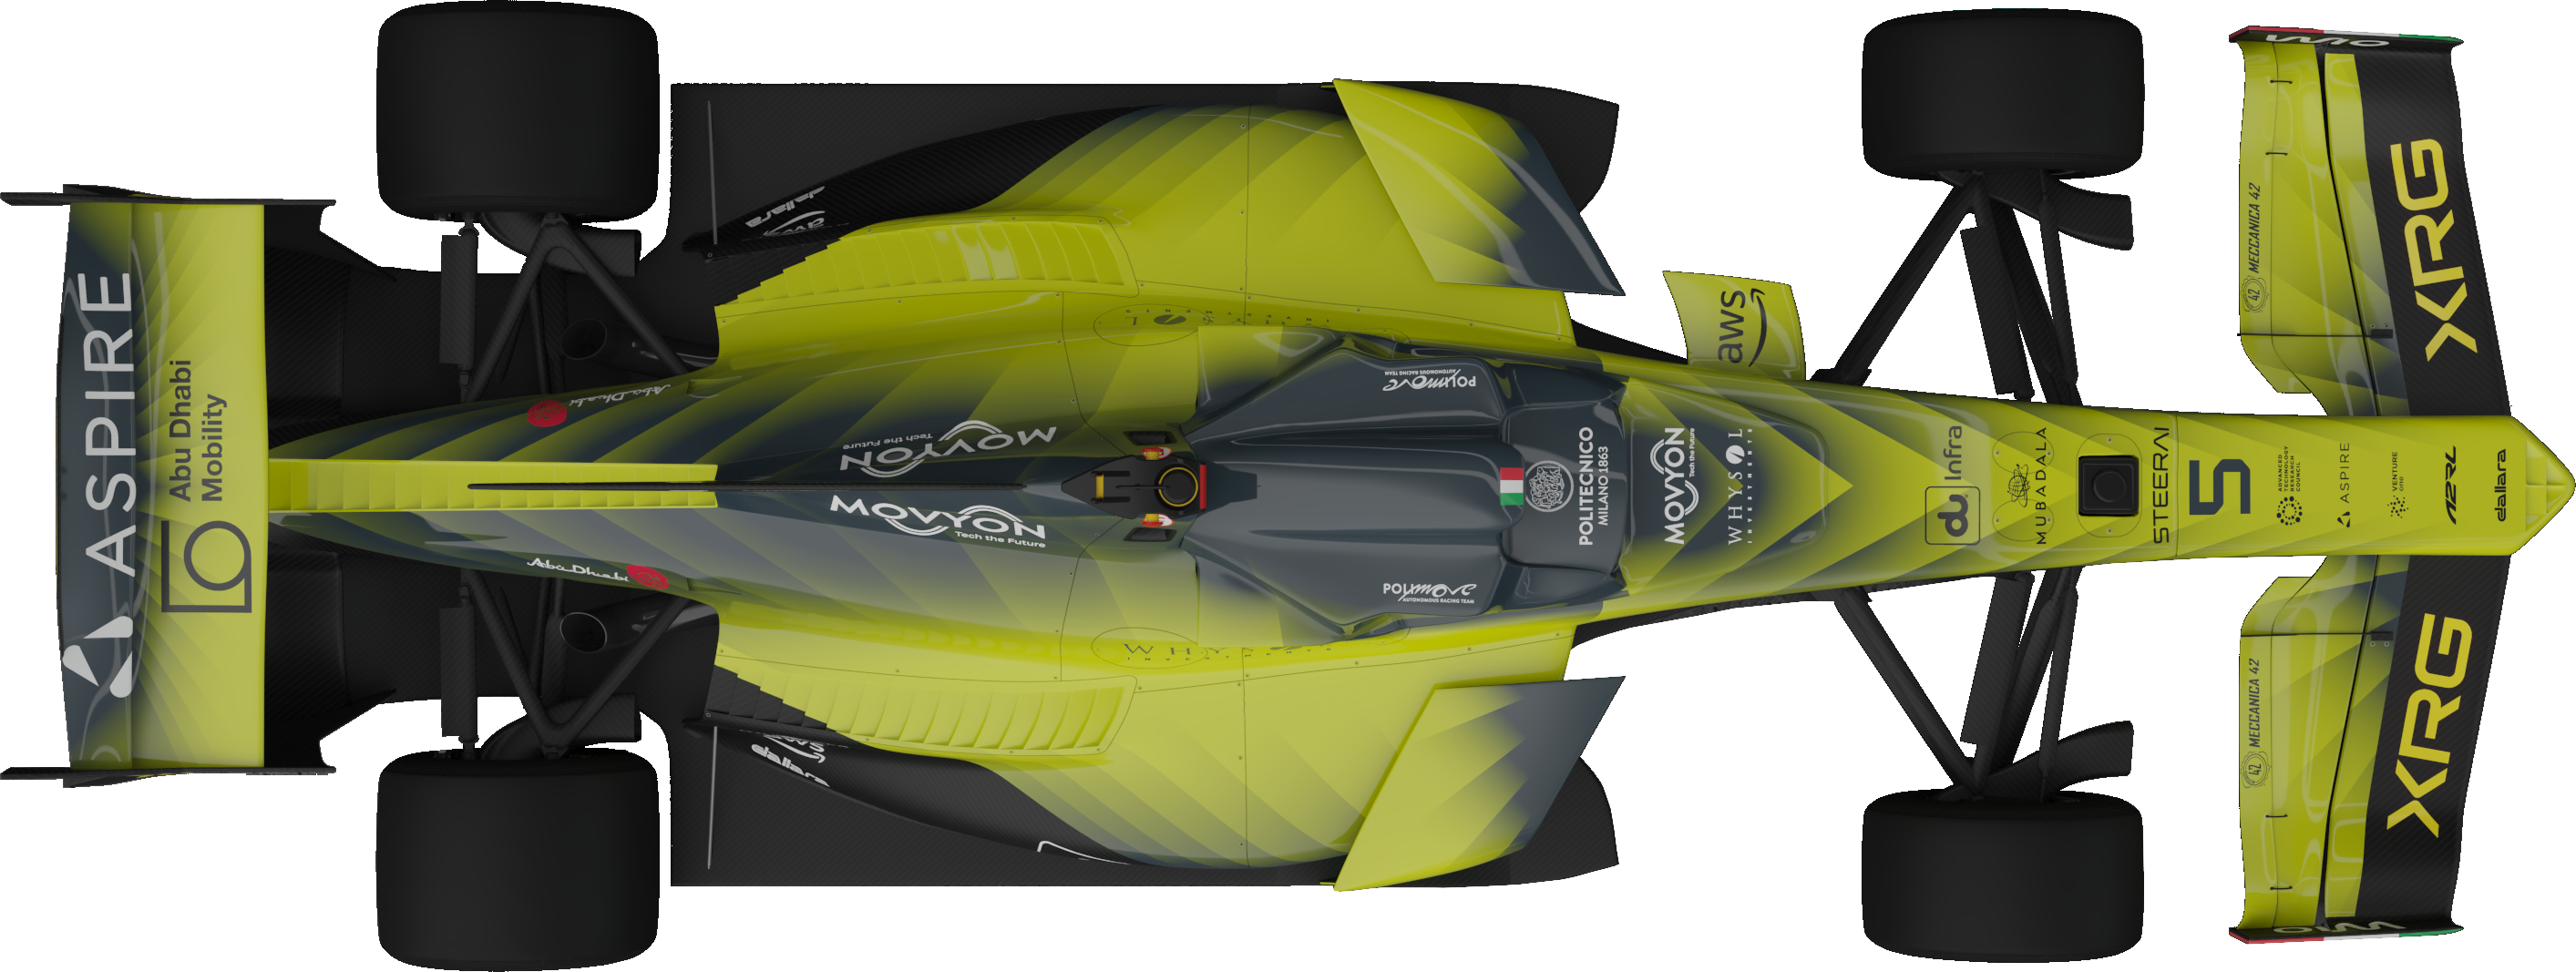
\includegraphics[width=30mm]{figures/ch2/src/eav24_top.png}}};
\draw[line] (act) -- (car);
\draw[line] (car) -| (S.south);
\end{tikzpicture}

    \caption{Main modules of the autonomous driving software and data exchanged between
    them.}
    \label{fig:sw_arch}
\end{figure}

\paragraph{Estimation.} The estimation module estimates the state of the ego
vehicle, i.e.\ its position, heading, velocity and acceleration, by
fusing the measurements of the GNSS receivers, of the inertial units and of the
proprioceptive sensors. Its output is used by the perception, planning and control
modules.

\paragraph{Perception.} The perception module turns the raw data of LiDARs, RaDARs and
cameras into a description of the vehicles around the ego car. A first stage processes
the data of each sensor separately: point clouds, RaDAR reflections and images are
filtered, the points belonging to other vehicles are isolated and a list of
\emph{detections} is produced, each one containing the position of a vehicle and, for
the RaDAR, its range rate. The detections of the different sensors are then passed to
the \emph{target tracking} module, which associates them over time with the vehicles
already known, fuses the information coming from the different sensors and estimates
the state of each opponent, including quantities that are not measured directly. The result is
the list of the opponents with their estimated state, which is the output of perception towards planning. The target
tracking module is the subject of this thesis and is described in detail in
Chapter~\ref{ch:tracking}.

\paragraph{Planning.} It receives the ego state from estimation, the opponent list
from perception and the data of a track database, which contains the
boundaries of the track and a set of reference trajectories. Based on the presence of
other vehicles and on the chosen strategy, i.e.\ following, overtaking or defending,
the planning module decides the trajectory that the vehicle has to follow; the
trajectory can also be selected by configuration. The output is a reference trajectory,
i.e.\ a path with the associated speed profile, which is sent to control.

\paragraph{Control.} It receives the reference trajectory from planning and the ego
state from estimation, and computes the commands for the actuators through two
controllers: a longitudinal controller, which acts on throttle, brake and gear to track
the reference speed, and a lateral controller, which computes the steering angle that
keeps the vehicle on the reference path.


\FloatBarrier

% =====================================================================
%  Chapter 3 - Target Tracking Pipeline
% =====================================================================

\chapter{Target Tracking Pipeline}
\label{ch:tracking}

This chapter is focused on describing the main characteristics of the target
tracking module. The objective of the algorithm is to estimate, at every instant, the state
of the opponents around the ego vehicle, i.e.\ their position, speed, heading and
acceleration, starting from the detections produced by the perception stage of each
sensor. As anticipated in Section~\ref{sec:sw_arch}, the list of the opponents with their
estimated state is the output of the perception module and becomes the input of the
planning module.

The estimation of the state of each opponent follows the structure of an Extended Kalman
Filter (EKF), the latter chosen to handle the nonlinearities of the dynamic model that
describes the motion of the vehicle. The filter alternates two essential steps: the
\emph{prediction}, in which the state is propagated in time according to a Constant
Curvature and Acceleration (CCA) model, and the \emph{update}, in which the predicted
state is corrected when a new measurement becomes available. Around the filter, the
target tracking module manages all the operations required to work with real
detections: the association of each measurement with the corresponding opponent, the
handling of the measurements that arrive out of sequence (OOSM), and the management of
the tracks, i.e.\ their creation, confirmation and deletion.

\begin{figure}[H]
    \centering
    \resizebox{\textwidth}{!}{% Block diagram of the target tracking pipeline (Chapter 3).
\begin{tikzpicture}[
    font=\footnotesize,
    >={Stealth[length=2mm]},
    blk/.style={draw, rounded corners=2pt, align=center, minimum height=10mm, inner sep=3pt},
    io/.style={blk, minimum width=18mm, fill=gray!8},
    mod/.style={blk, minimum width=20mm, fill=blue!6},
    ekf/.style={blk, minimum width=20mm, fill=blue!18, very thick},
    grp/.style={draw, dashed, rounded corners=4pt, inner sep=5pt},
    lab/.style={font=\scriptsize, align=center, text=black!70},
    line/.style={->, thick}
]
% main chain
\node[mod] (oosm) {OOSM\\handling};
\node[io, left=20mm of oosm] (perc) {Perception\\pipelines};
\node[ekf, right=9mm of oosm] (pred) {Prediction\\(CCA model)};
\node[mod, right=9mm of pred] (assoc) {Data association\\(Mahalanobis,\\Munkres)};
\node[ekf, right=12mm of assoc] (upd) {Update\\(correction)};
\node[blk, minimum width=16mm, right=9mm of upd] (tracks) {Tracks};
\node[mod, below=9mm of upd] (mgmt) {Track management\\(creation, confirmation,\\deletion)};

% external inputs and output
\node[io, above=9mm of perc] (raw) {Sensors\\(LiDAR, RaDAR,\\camera)};
\node[io, above=9mm of pred] (db) {Track\\database};
\node[io, above=9mm of assoc] (ego) {Ego state\\(estimation)};
\node[io, above=9mm of tracks] (plan) {Planning};

% data flow
\draw[line] (raw) -- node[lab, right]{raw data} (perc);
\draw[line] (perc) -- node[lab, above, pos=0.4]{detections} (oosm);
\draw[line] (oosm) -- node[lab, above]{$\mathbf{z},\,t_s$} (pred);
\draw[line] (pred) -- (assoc);
\draw[line] (assoc) -- node[lab, above]{assigned} (upd);
\draw[line] (assoc.south) |- node[lab, above, pos=0.75]{unassigned} (mgmt.west);
\draw[line] (upd) -- (tracks);
\draw[line] (mgmt.east) -| (tracks.south);
\draw[line] (db) -- node[lab, right]{curvature $\kappa$} (pred);
\draw[line] (ego) -- node[lab, right]{ego pose at $t_s$} (assoc);
\draw[line] (tracks) -- node[lab, right]{opponents} (plan);

% feedback: the tracks are the starting point of the next prediction
\coordinate (fb) at ($(mgmt.south)+(0,-5mm)$);
\coordinate (fbr) at ($(tracks.east)+(5mm,0)$);
\draw[line] (tracks.east) -- (fbr) |- (fb) -| node[lab, above, pos=0.25]{$\hat{\mathbf{x}},\,\mathbf{P}$ of the tracks} (pred.south);

\node[grp, fit=(oosm)(pred)(assoc)(upd)(tracks)(mgmt)(fb)(fbr), label={[lab]below:Target tracking}] {};
\end{tikzpicture}
}
    \caption{Main steps of the target tracking pipeline.}
    \label{fig:tt_pipeline}
\end{figure}

Following the same pipeline; Section~\ref{sec:tt_prediction}
describes the prediction step of the EKF. Section~\ref{sec:tt_association} explains how
each measurement is associated with the corresponding track, leveraging on the Mahalanobis
distance gating and the Munkres algorithm, and how the measurements that arrive out of sequence
are handled. Section~\ref{sec:tt_correction} presents the measurement models and the
update step, in which the predicted state is corrected with the associated measurement.
Section~\ref{sec:tt_management} is about tracks management. Finally,
Section~\ref{sec:tt_baseline} overviews the main performance limits of the current
pipeline, highlighting estimate degradation in rapidly changing dynamic conditions, i.e.\ the starting point of the research work.

% =====================================================================
\section{Prediction}
\label{sec:tt_prediction}

The prediction step propagates the state of each track, together with its uncertainty,
from the time of the last update to the time of the next measurement, according to a
model of the motion of the opponent.

\subsection{Prediction Step}
\label{subsec:tt_prediction}

The EKF describes the evolution of the state of the opponent and its relation with the
measurements through the discrete-time nonlinear system
\begin{equation}
    \begin{aligned}
        \mathbf{x}_{k+1} &= f_d(\mathbf{x}_k) + \mathbf{w}_k, \\
        \mathbf{z}_k &= h(\mathbf{x}_k) + \mathbf{v}_k,
    \end{aligned}
    \label{eq:tt_system}
\end{equation}
where $f_d(\cdot)$ is the motion model, which propagates the state $\mathbf{x}_k$ over the
interval between two filter iterations, and $h(\cdot)$ is the measurement model, which
depends on the sensor that produced the measurement $\mathbf{z}_k$
(Section~\ref{sec:tt_correction}). The process noise $\mathbf{w}_k$ represents the
confidence in the motion model, i.e.\ how reliable the prediction is expected to be,
while the measurement noise $\mathbf{v}_k$ represents the accuracy of the measurement; both are modelled as zero-mean Gaussian white noises, with covariance
matrices $\mathbf{Q}_k$ and $\mathbf{R}_k$ respectively.

Since $f_d$ is nonlinear, it is linearized around the last estimate,
\begin{equation}
    \mathbf{F}_k = \left.\frac{\partial f_d}{\partial \mathbf{x}}\right|_{\hat{\mathbf{x}}_k}.
    \label{eq:tt_F_def}
\end{equation}
The estimated state $\hat{\mathbf{x}}$ is associated with a measure of its uncertainty,
represented by the covariance matrix $\mathbf{P}$ of the filter. Given the estimate
$\hat{\mathbf{x}}_k$ and its covariance $\mathbf{P}_k$, the prediction step computes the a
priori estimate and covariance at the next iteration,
\begin{equation}
    \begin{aligned}
        \hat{\mathbf{x}}_{k+1|k} &= f_d(\hat{\mathbf{x}}_k), \\
        \mathbf{P}_{k+1|k} &= \mathbf{F}_k\,\mathbf{P}_k\,\mathbf{F}_k^\top + \mathbf{Q}_k,
    \end{aligned}
    \label{eq:tt_prediction}
\end{equation}
where the covariance is propagated forward with the motion model and increased by the
contribution of the process noise.

In the target tracking module the prediction step is performed either when a new
measurement is received, in which case the state is predicted to the validity time of
the measurement, or when a given time has elapsed since the last iteration, so that the
estimate is kept up to date also in the absence of measurements. Since the measurements
come from different sensors, with different update rates and latencies, the interval
$\Delta t = t_{k+1} - t_k$ between two consecutive predictions is not constant. For this
reason the discrete-time equations used to propagate the state and the process noise are
derived through an exact discretization of the continuous-time model, which is valid for
any value of $\Delta t$ and is described in Section~\ref{subsec:tt_cca}.

\subsection{Constant Curvature and Acceleration Model}
\label{subsec:tt_cca}

The motion of the opponent is described by a Constant Curvature and Acceleration (CCA)
model. The state of each opponent is defined as
\begin{equation}
    \renewcommand{\arraystretch}{1.3}\setlength{\jot}{8pt}
    \mathbf{x} = \begin{bmatrix} x & y & v & a & \psi \end{bmatrix}^\top,
    \label{eq:tt_state}
\end{equation}
where $(x,\,y)$ is the position of the opponent, $v$ its speed, $a$ its longitudinal
acceleration and $\psi$ its heading.

\paragraph{Continuous-time model.} The CCA model assumes that, over a prediction
interval, the opponent travels along a path of constant curvature $\kappa$ with a constant
longitudinal acceleration. The continuous-time dynamics are
\begin{equation}
    \renewcommand{\arraystretch}{1.3}\setlength{\jot}{8pt}
    \left\{
    \begin{aligned}
        \dot x(t)    &= v(t)\cos\psi(t), \\
        \dot y(t)    &= v(t)\sin\psi(t), \\
        \dot v(t)    &= a(t), \\
        \dot a(t)    &= 0, \\
        \dot\psi(t)  &= \kappa\,v(t),
    \end{aligned}
    \right.
    \label{eq:tt_cca}
\end{equation}
where the yaw rate is expressed as $\dot\psi = \kappa\,v$: once the path is fixed, the
rotation of the vehicle depends only on how fast it travels along it. In compact form,
the system is written as $\dot{\mathbf{x}}(t) = f(\mathbf{x}(t),\kappa)$.

The a priori knowledge of the trajectories that the opponent may follow, i.e.\ the racing
lines stored in the track database introduced in Section~\ref{sec:sw_arch}, is exploited
as a prior and modelled as an external input: the curvature $\kappa$ is not estimated by
the filter, but read from the database. At every prediction the point closest to the estimated position of the opponent
is searched on the optimal trajectory, starting from the index found at the previous step;
if its distance from the opponent exceeds \SI{0.5}{m}, the search is extended to all the
other trajectories of the database, and the curvature of the closest point is used for
the prediction.

\paragraph{Discrete-time model.} Starting from the continuous-time
model~\eqref{eq:tt_cca}, the discrete-time motion model is obtained through its exact
discretization,
\begin{equation}
    \renewcommand{\arraystretch}{1.3}\setlength{\jot}{8pt}
    \mathbf{x}_{k+1} = \mathbf{x}_k
    + \int_{t_k}^{t_{k+1}} f(\mathbf{x}(\tau),\kappa)\,\mathrm{d}\tau.
    \label{eq:tt_exact_disc}
\end{equation}
Under the assumption of constant curvature and acceleration over the interval, the
integrals can be solved in closed form. For acceleration, speed and heading,
\begin{equation}
    \renewcommand{\arraystretch}{1.3}\setlength{\jot}{8pt}
    \begin{aligned}
        a_{k+1}    &= a_k + \int_{t_k}^{t_{k+1}} 0\,\mathrm{d}\tau = a_k, \\
        v_{k+1}    &= v_k + \int_{t_k}^{t_{k+1}} a_k\,\mathrm{d}\tau = v_k + a_k\,\Delta t, \\
        \psi_{k+1} &= \psi_k + \int_{t_k}^{t_{k+1}} \kappa\,v(\tau)\,\mathrm{d}\tau
                    = \psi_k + \kappa\left(v_k\,\Delta t + \tfrac{1}{2}\,a_k\,\Delta t^2\right),
    \end{aligned}
    \label{eq:tt_cca_vapsi}
\end{equation}
while, since $\mathrm{d}\psi = \kappa\,v\,\mathrm{d}\tau$, the integrals of the position
reduce to integrals in the heading,
\begin{equation}
    \renewcommand{\arraystretch}{1.3}\setlength{\jot}{8pt}
    \begin{aligned}
        x_{k+1} &= x_k + \int_{t_k}^{t_{k+1}} v(\tau)\cos\psi(\tau)\,\mathrm{d}\tau
                 = x_k + \frac{\sin\psi_{k+1} - \sin\psi_k}{\kappa}, \\
        y_{k+1} &= y_k + \int_{t_k}^{t_{k+1}} v(\tau)\sin\psi(\tau)\,\mathrm{d}\tau
                 = y_k - \frac{\cos\psi_{k+1} - \cos\psi_k}{\kappa}.
    \end{aligned}
    \label{eq:tt_cca_xy}
\end{equation}
The discrete-time motion model is therefore
\abovedisplayskip=16pt plus 3pt minus 3pt \belowdisplayskip=16pt plus 3pt minus 3pt
\abovedisplayshortskip=16pt plus 3pt minus 3pt \belowdisplayshortskip=16pt plus 3pt minus 3pt
\begin{equation}
    \renewcommand{\arraystretch}{1.3}\setlength{\jot}{8pt}
    f_d(\mathbf{x}_k) =
    \begin{bmatrix}
        x_k + \dfrac{\sin\psi_{k+1} - \sin\psi_k}{\kappa} \\[2ex]
        y_k - \dfrac{\cos\psi_{k+1} - \cos\psi_k}{\kappa} \\[2ex]
        v_k + a_k\,\Delta t \\
        a_k \\
        \psi_k + \kappa\left(v_k\,\Delta t + \tfrac{1}{2}\,a_k\,\Delta t^2\right)
    \end{bmatrix}.
    \label{eq:tt_cca_discrete}
\end{equation}
When the curvature tends to zero, the opponent travels along a straight line and the
model reduces to
\abovedisplayskip=16pt plus 3pt minus 3pt \belowdisplayskip=16pt plus 3pt minus 3pt
\abovedisplayshortskip=16pt plus 3pt minus 3pt \belowdisplayshortskip=16pt plus 3pt minus 3pt
\begin{equation}
    \renewcommand{\arraystretch}{1.3}\setlength{\jot}{8pt}
    \lim_{\kappa \to 0} f_d(\mathbf{x}_k) =
    \begin{bmatrix}
        x_k + \left(v_k\,\Delta t + \tfrac{1}{2}\,a_k\,\Delta t^2\right)\cos\psi_k \\
        y_k + \left(v_k\,\Delta t + \tfrac{1}{2}\,a_k\,\Delta t^2\right)\sin\psi_k \\
        v_k + a_k\,\Delta t \\
        a_k \\
        \psi_k
    \end{bmatrix},
    \label{eq:tt_cca_straight}
\end{equation}
which is used when $|\kappa| < \SI{e-4}{m^{-1}}$ to avoid the division by zero
in~\eqref{eq:tt_cca_discrete}.

Applying~\eqref{eq:tt_F_def} to~\eqref{eq:tt_cca_discrete}, the linearized state matrix
used in the prediction of the covariance is
\abovedisplayskip=16pt plus 3pt minus 3pt \belowdisplayskip=16pt plus 3pt minus 3pt
\abovedisplayshortskip=16pt plus 3pt minus 3pt \belowdisplayshortskip=16pt plus 3pt minus 3pt
\begin{equation}
    \renewcommand{\arraystretch}{1.3}\setlength{\jot}{8pt}
    \mathbf{F}_k =
    \begin{bmatrix}
        1 & 0 & \Delta t\cos\psi_{k+1} & \tfrac{1}{2}\Delta t^2\cos\psi_{k+1} & \dfrac{\cos\psi_{k+1} - \cos\psi_k}{\kappa} \\[2ex]
        0 & 1 & \Delta t\sin\psi_{k+1} & \tfrac{1}{2}\Delta t^2\sin\psi_{k+1} & \dfrac{\sin\psi_{k+1} - \sin\psi_k}{\kappa} \\[2ex]
        0 & 0 & 1 & \Delta t & 0 \\
        0 & 0 & 0 & 1 & 0 \\
        0 & 0 & \kappa\,\Delta t & \tfrac{1}{2}\kappa\,\Delta t^2 & 1
    \end{bmatrix},
    \label{eq:tt_F}
\end{equation}
while, in the straight-line case~\eqref{eq:tt_cca_straight}, it becomes
\abovedisplayskip=16pt plus 3pt minus 3pt \belowdisplayskip=16pt plus 3pt minus 3pt
\abovedisplayshortskip=16pt plus 3pt minus 3pt \belowdisplayshortskip=16pt plus 3pt minus 3pt
\begin{equation}
    \renewcommand{\arraystretch}{1.3}\setlength{\jot}{8pt}
    \mathbf{F}_k =
    \begin{bmatrix}
        1 & 0 & \Delta t\cos\psi_k & \tfrac{1}{2}\Delta t^2\cos\psi_k & -\left(v_k\,\Delta t + \tfrac{1}{2}\,a_k\,\Delta t^2\right)\sin\psi_k \\
        0 & 1 & \Delta t\sin\psi_k & \tfrac{1}{2}\Delta t^2\sin\psi_k & \phantom{-}\left(v_k\,\Delta t + \tfrac{1}{2}\,a_k\,\Delta t^2\right)\cos\psi_k \\
        0 & 0 & 1 & \Delta t & 0 \\
        0 & 0 & 0 & 1 & 0 \\
        0 & 0 & 0 & 0 & 1
    \end{bmatrix}.
    \label{eq:tt_F_straight}
\end{equation}
All the quantities in~\eqref{eq:tt_F} and~\eqref{eq:tt_F_straight} are evaluated at the
last estimate $\hat{\mathbf{x}}_k$.

\paragraph{Process noise.} Two sources of uncertainty are considered. The first is the
variation of the acceleration, which the model assumes constant: a white noise $w_a$ with
spectral density $q_a$ acts on its derivative, so that the acceleration evolves as a
random walk and can follow the braking and traction phases. The second is the
uncertainty of the curvature read from the database: since the set of trajectories that
the opponent may follow is used as prior information, this uncertainty is lower, but it
accounts for the small differences between the actual trajectory of the opponent and the
one prescribed by the database. A white perturbation $w_\kappa$ of the curvature, with
spectral density $q_\kappa$, produces an error $v\,w_\kappa$ on the yaw rate. The
continuous-time model with process noise becomes
\abovedisplayskip=16pt plus 3pt minus 3pt \belowdisplayskip=16pt plus 3pt minus 3pt
\abovedisplayshortskip=16pt plus 3pt minus 3pt \belowdisplayshortskip=16pt plus 3pt minus 3pt
\begin{equation}
    \renewcommand{\arraystretch}{1.3}\setlength{\jot}{8pt}
    \dot{\mathbf{x}}(t) = f(\mathbf{x}(t),\kappa) + \mathbf{G}\,\mathbf{w}(t),
    \qquad
    \mathbf{G} =
    \begin{bmatrix}
        0 & 0 & 0 & 0 & v \\
        0 & 0 & 0 & 1 & 0
    \end{bmatrix}^\top,
    \qquad
    \mathbf{Q}_c = \begin{bmatrix} q_\kappa & 0 \\ 0 & q_a \end{bmatrix},
    \label{eq:tt_noise}
\end{equation}
where $\mathbf{w} = [w_\kappa,\,w_a]^\top$ and $\mathbf{Q}_c$ is its spectral density
matrix. The discrete-time process noise covariance is obtained through the exact
discretization of the noise, i.e.\ by integrating its effect over the prediction interval
through the linearized dynamics,
\abovedisplayskip=16pt plus 3pt minus 3pt \belowdisplayskip=16pt plus 3pt minus 3pt
\abovedisplayshortskip=16pt plus 3pt minus 3pt \belowdisplayshortskip=16pt plus 3pt minus 3pt
\begin{equation}
    \renewcommand{\arraystretch}{1.3}\setlength{\jot}{8pt}
    \mathbf{Q}_k = \int_0^{\Delta t} e^{\mathbf{A}\tau}\,\mathbf{G}\,\mathbf{Q}_c\,
        \mathbf{G}^\top e^{\mathbf{A}^\top\tau}\,\mathrm{d}\tau,
    \label{eq:tt_Q_def}
\end{equation}
where $\mathbf{A}$ is the Jacobian of the continuous-time dynamics~\eqref{eq:tt_cca},
evaluated at the last estimate,
\abovedisplayskip=16pt plus 3pt minus 3pt \belowdisplayskip=16pt plus 3pt minus 3pt
\abovedisplayshortskip=16pt plus 3pt minus 3pt \belowdisplayshortskip=16pt plus 3pt minus 3pt
\begin{equation}
    \renewcommand{\arraystretch}{1.3}\setlength{\jot}{8pt}
    \mathbf{A} = \left.\frac{\partial f}{\partial \mathbf{x}}\right|_{\hat{\mathbf{x}}_k} =
    \begin{bmatrix}
        0 & 0 & \cos\psi & 0 & -v\sin\psi \\
        0 & 0 & \sin\psi & 0 & \phantom{-}v\cos\psi \\
        0 & 0 & 0 & 1 & 0 \\
        0 & 0 & 0 & 0 & 0 \\
        0 & 0 & \kappa & 0 & 0
    \end{bmatrix}.
    \label{eq:tt_A}
\end{equation}
The integral is solved analytically, and the resulting closed-form expressions of the
elements of $\mathbf{Q}_k$, which depend on $v$, $\psi$, $\kappa$ and $\Delta t$, are
evaluated at every prediction. The result is a full $5 \times 5$ matrix: although the
noise acts directly only on the acceleration and on the heading, it propagates
indirectly to the other states through the integration of the dynamics. The two spectral
densities $q_\kappa$ and $q_a$ are the tuning parameters of the model, and their ratio
with respect to the measurement noise sets how much the filter relies on the prediction
rather than on the measurements.

% =====================================================================
\section{Data Association}
\label{sec:tt_association}

\subsection{Mahalanobis Distance}
\label{subsec:tt_mahalanobis}

\subsection{Munkres Algorithm}
\label{subsec:tt_munkres}

\subsection{Out-of-Sequence Measurements}
\label{subsec:tt_oosm}

% =====================================================================
\section{Correction}
\label{sec:tt_correction}

\subsection{Measurement Model}
\label{subsec:tt_meas_model}

\subsection{Measurement Noise}
\label{subsec:tt_meas_noise}

\subsection{Update}
\label{subsec:tt_update}

% =====================================================================
\section{Track Management}
\label{sec:tt_management}

% =====================================================================
\section{Baseline Performance}
\label{sec:tt_baseline}

\FloatBarrier

\chapter{Measurement Noise Analysis}
\label{ch:adaptive_r}

In this chapter,  an in depth analysis and characterization of the measurement noise of the sensors introduced in
Chapter~\ref{ch:tracking} is presented. The latter is of particular relevance  because the covariance of the measurement noise regulates the correction step of the Kalman
filter and, therefore, the quality of the estimate. A covariance that is too large
under uses the information carried by the measurements, while one that is too small
weights them too much making the estimate too noisy.

The chapter is divided into two parts. The first part aims at characterizing the
measurement noise of the sensors. The errors of each source are analyzed, the errors related to the
setup are compensated and the global trends of each sensor are identified, so that
only the random part of the error has to be described by the measurement noise
covariance, and each measurement is weighted correctly by the filter.

The second part introduces a covariance matching technique for the measurement noise
covariance. This technique adapts the matrix $\mathbf{R}$ online, using the information
contained in the innovations of the filter, in order to handle the local trends of the
standard deviation of the measurement errors, which can increase, e.g.\ due to a partial
occlusion of the opponent or to a degradation of the sensors, or decrease, e.g.\ when the
opponent is stationary.

Section~\ref{sec:preprocessing} describes the pre-processing of the data, i.e.\ the
reconstruction of the ground truth and the reference frames of the errors, and
Section~\ref{sec:datasets} analyzes the datasets. Section~\ref{sec:deterministic} addresses the errors related to the
setup, Section~\ref{sec:macro} the global error trends of each sensor, and
Sections~\ref{sec:gaussian_fit} and~\ref{sec:gauss_markov} the residual errors, through
their Gaussian fit and their local behavior.
Section~\ref{sec:adaptive_r} presents the adaptive approach and
Section~\ref{sec:ch4_results} the results.

% =====================================================================
\section{Pre-processing}
\label{sec:preprocessing}

The analysis of the measurement errors requires each detection to be compared with the
true position of the opponent at the instant in which it was acquired. This section
describes how the reference trajectory of the opponent is obtained and synchronized with
the detections, how the detections are associated with it, and in which reference frames
the resulting errors are expressed.

\subsection{Ground Truth Reconstruction}
\label{sec:gt}

The reference for the state of the opponent is the state estimated by the opponent
vehicle itself. During the sessions, each team records the output of its own state
estimation, based on RTK-GNSS receivers and inertial units, and shares it after the
session. For each sample, the data contain the timestamp, the position and the heading of
the vehicle, its longitudinal speed and, when available, its longitudinal acceleration.
Since each team adopts its own format and reference system, the data are first brought
into a common structure, compatible with the logs of the ego vehicle. The position and
the heading of the opponent are roto-translated into the map frame of the ego vehicle, so that the two vehicles are
described with respect to the same origin and orientation.

When the longitudinal acceleration is measured by the
inertial unit of the opponent, it is low-pass filtered with a zero-phase Butterworth
filter (2nd order filter); otherwise, it is
obtained by differentiating the speed and smoothing the result with a Savitzky-Golay
filter. The yaw rate, when not provided, is obtained in the same way from the heading.

To compute the relative geometry of the two vehicles, each sample of the opponent is
associated with the sample of the ego vehicle with the closest timestamp. For each pair of
synchronized samples, the position of
the opponent in the frame of the ego vehicle is obtained by rotating the relative position
by the heading $\psi_e$ of the ego vehicle,
\begin{equation}
    \mathbf{p}_{\mathrm{rel}} =
    \begin{bmatrix} x_{\mathrm{rel}} \\ y_{\mathrm{rel}} \end{bmatrix}
    = \mathbf{R}(\psi_e)^\top \left(\mathbf{p}_o - \mathbf{p}_e\right),
    \qquad
    \psi_{\mathrm{rel}} = \psi_o - \psi_e,
    \label{eq:gt_rel}
\end{equation}
where $\mathbf{p}_o$, $\mathbf{p}_e$ and $\psi_o$, $\psi_e$ are the positions and the
headings of opponent and ego vehicle in the map frame, and $\mathbf{R}(\cdot)$ is the
rotation matrix defined in~\eqref{eq:tt_R_rot}. The range is the distance between the
two vehicles, $\rho = \|\mathbf{p}_o - \mathbf{p}_e\|$, and the range rate is the
projection of the relative velocity on the line of sight,
\begin{equation}
    \dot\rho = \frac{\left(\mathbf{p}_o - \mathbf{p}_e\right)^\top
    \left(\mathbf{v}_o - \mathbf{v}_e\right)}{\rho},
    \qquad
    \mathbf{v}_i = v_i \begin{bmatrix} \cos\psi_i \\ \sin\psi_i \end{bmatrix},
    \quad i \in \{o,\,e\},
    \label{eq:gt_rhodot}
\end{equation}
with $v_o$ and $v_e$ the speeds of the two vehicles.

It is important to note that the reference carries its own mistakes. As stated at the beginning of the section, it coincides with the output of the state estimation pipeline of the opponent, and its quality is therefore strictly related to the performance of that pipeline: a degradation of the GNSS measurements, as well as any other error of the estimate, is directly inherited by the reference. Moreover, since each opponent adopts its own pipeline, the quality of the reference can differ from one opponent to another.

\subsection{Reference Frames of the Errors}
\label{subsec:err_frames}

Once the reference has been reconstructed, to compute the measurement errors, we first need to associate the ground
truth and the measurements of the sensors. The ground truth is available at
a higher frequency than the detections, therefore, it is linearly interpolated at the acquisition time of each detection. The measurement error is
then the difference between the position of the detection and the position of the
opponent given by the ground truth at the same instant.

The errors are expressed in the frame of the ego vehicle,
\begin{equation}
    \mathbf{e} =
    \begin{bmatrix} e_x \\ e_y \end{bmatrix}
    = \mathbf{R}(\psi_e)^\top \left(\mathbf{p}_{\mathrm{det}} - \mathbf{p}_{\mathrm{gt}}\right),
    \label{eq:err_ego}
\end{equation}
where $\mathbf{p}_{\mathrm{det}}$ and $\mathbf{p}_{\mathrm{gt}}$ are the positions of the
detection and of the ground truth in the map frame, and $\psi_e$ is the heading of the ego
vehicle, consistently with~\eqref{eq:gt_rel}. This frame is attached to the ego vehicle,
so its axes keep the same meaning along the whole lap: $x_{\mathrm{rel}}$ is always
positive ahead of the ego vehicle and $y_{\mathrm{rel}}$ positive to its left. As a
consequence, $e_x$ is always the error along the longitudinal direction of the ego vehicle
and $e_y$ the lateral one, regardless of the absolute orientation of the vehicles in the
map, and the errors collected along the lap can be compared and aggregated consistently.

\FloatBarrier

% =====================================================================
\section{Dataset Analysis}
\label{sec:datasets}

This section provides an analysis of the main characteristics of the datasets used in
the following sections. The main considerations derive from two sessions, recorded on 26 July
2026 and on 3 August 2026 at the Autodromo Internazionale Enzo e Dino Ferrari in Imola,
with two different opponents, TUM and Kinetiz, and referred to in the following as
session 07/26\_TUM and session 08/03\_Kinetiz. These sessions are used to identify the
setup-related errors, in Section~\ref{sec:deterministic}, and the global error trends of
each sensor, in Section~\ref{sec:macro}.

The data acquired during the test sessions carried out in October 2026 at the Yas Marina
Circuit in Abu Dhabi are then used to validate these findings. In these sessions, the
teams had the possibility to test with two vehicles at the same time. Using the state
estimation of the team as reference, whose conventions on the reference frame and whose
uncertainty are known, the errors of the perception pipeline can be isolated from those
of the reference.

The main characteristics of the two sessions at Imola are summarized in
Table~\ref{tab:sessions}.

\begin{table}[H]
    \centering
    \small
    \begin{tabular}{lcc}
        \toprule
                                             & Session 07/26\_TUM            & Session 08/03\_Kinetiz            \\
        \midrule
        Date                                 & 26/07/2026              & 03/08/2026              \\
        Opponent                             & TUM                     & Kinetiz                 \\
        Duration                             & \SI{1261}{s}            & \SI{1780}{s}            \\
        Distance covered by the opponent     & \SI{29.2}{km} (6 laps)  & \SI{43.3}{km} (9 laps)  \\
        Median / maximum speed of the opponent & \SI{90}{} / \SI{163}{km/h} & \SI{91}{} / \SI{156}{km/h} \\
        Opponent stationary                  & \SI{139}{s}             & \SI{74}{s}              \\
        Opponent ahead of the ego vehicle    & \SI{72}{\percent}       & \SI{35}{\percent}       \\
        Position swaps                       & 1                       & 7                       \\
        Median range                         & \SI{48.5}{m}            & \SI{49.2}{m}            \\
        Median lateral position $y_{\mathrm{rel}}$ & \SI{6.0}{m}       & \SI{-5.7}{m}            \\
        \bottomrule
    \end{tabular}
    \caption{Main characteristics of the two sessions. }
    \label{tab:sessions}
\end{table}

Both sessions cover a wide range of dynamic conditions. The opponent travels at a median
speed of about \SI{90}{km/h} and reaches more than \SI{150}{km/h}, alternating braking,
cornering and traction phases along the lap. The two sessions also include several safe
stops, during which the opponent is stationary; these intervals are of particular interest since they allow the errors to be
characterized also in static conditions. Session 08/03\_Kinetiz also contains seven position swaps
between the vehicles. Overall, the combination of
safe stops, overtakes and laps at high speed ensures that the whole spectrum of the
dynamics of interest is covered by the datasets.

The sessions are also complementary in the relative geometry between the
vehicles. In session 07/26\_TUM the opponent is ahead of the ego vehicle for most of the time
and moves mainly on its left, both when ahead and when behind, with a median lateral
position of about \SI{6}{m}. In session 08/03\_Kinetiz the ego vehicle leads for most of the time,
and the opponent moves mainly on its right, with a median lateral position of about
\SI{-6}{m}.

Fig.~\ref{fig:ds_rate} shows the detection rate of each sensor as a
function of the range, separately for the opponent ahead of and behind the ego vehicle;
the rate is computed as the number of detections associated with the opponent in each
range interval divided by the time spent by the opponent in that interval. With the opponent ahead, both LiDAR pipelines detect it at close to the
nominal rate of \SI{10}{Hz} up to about \SI{50}{m}, and the rate decreases gradually with
the range, down to about \SI{100}{m} for both Clustering and PointPillars.
With the opponent behind, instead, the rate drops already beyond \SI{30}{m} and becomes
negligible beyond 50--\SI{60}{m}. This effect is due to the fact that, as the range increases,
the opponent approaches the longitudinal axis of the ego vehicle and enters the blind
spot caused by the rear wing (Section~\ref{subsec:lidar}). Only a small portion of the
opponent remains visible, and the few points returned are often not enough to produce a detection.  The RaDAR, mounted below the rear wing, does not suffer from this limitation and keeps detecting the
opponent behind up to \SI{150}{m}.

\begin{figure}[H]
    \centering
    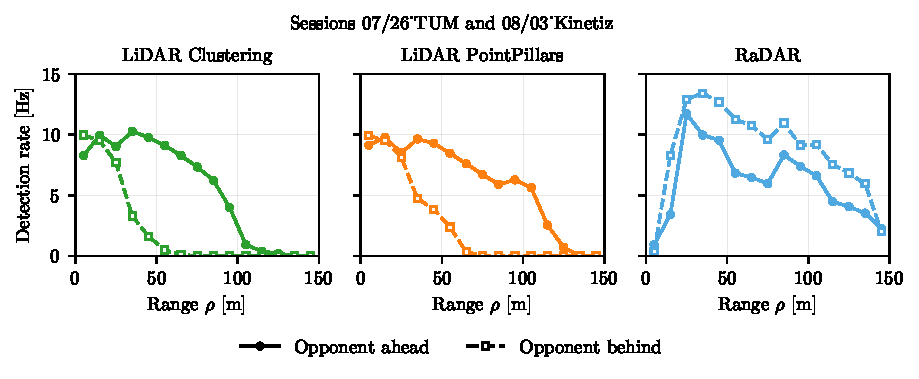
\includegraphics[width=\textwidth]{figures/ch4/detection_rate_range.pdf}
    \caption{Detection rate as a function of the range, with the opponent ahead and behind.}
    \label{fig:ds_rate}
\end{figure}

\FloatBarrier

% =====================================================================
\section{Setup-Related Errors}\label{sec:deterministic}

First of all, the errors related to the setup are taken into account. The latter, being systematic and repeatable, can be identified and compensated. 

\subsection{Longitudinal Component}
\label{subsec:det_long}

The analysis of the longitudinal component starts from the two LiDAR pipelines.
Fig.~\ref{fig:det_long} shows their longitudinal error in a window of session
07/26\_TUM: in both cases the error is centered on a constant bias, equal to
\SI{0.40}{m} for Clustering and to \SI{0.36}{m} for PointPillars.  

\begin{figure}[H]
    \centering
    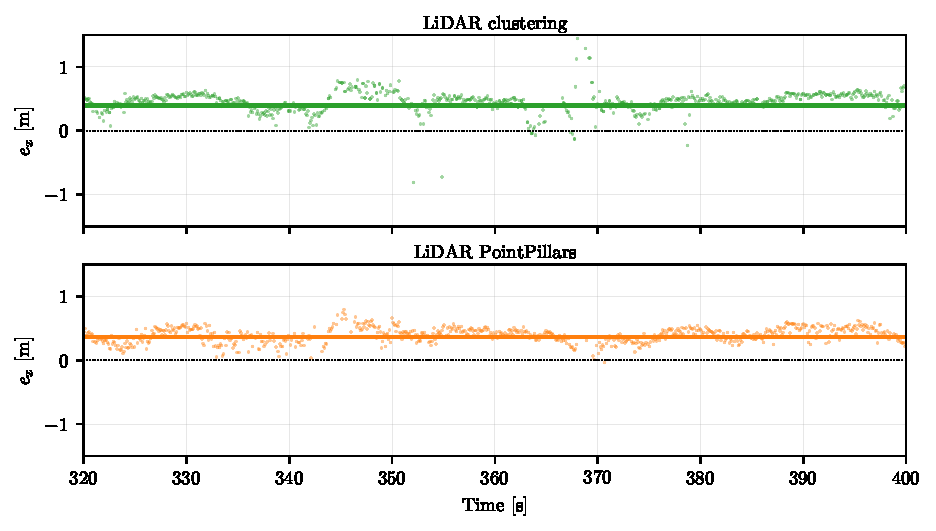
\includegraphics[width=\textwidth]{figures/ch4/det_long_time.pdf}
    \caption[Longitudinal error of the LiDARs]{Longitudinal error of the LiDARs in a window of session 07/26\_TUM, with the mean
    over the session: \SI{0.40}{m} for Clustering and \SI{0.36}{m} for PointPillars.}
    \label{fig:det_long}
\end{figure}

Moving to session 08/03\_Kinetiz, the  offset changes: the mean
longitudinal error is \SI{0.02}{m} for Clustering and \SI{0.09}{m} for PointPillars.
The sensors and the detection pipelines are the same in the two
sessions, while the opponent, and therefore the reference, changes. The first hypothesis is thus that the bias originates from the ground truth: if the
point to which the opponent refers its state estimate is shifted along its longitudinal
axis with respect to the point of the detections (Section~\ref{sec:gt}), the shift
appears as a constant bias of $e_x$.

The analysis is then extended to the longitudinal errors of the camera, shown in
Fig.~\ref{fig:det_cam} for session 07/26\_TUM. Beyond \SI{60}{m}, the error shows a clear
dependence on the range, so the analysis is restricted to the range 20--\SI{60}{m}. Within
this range, the camera shares the same bias as the LiDARs in both sessions
(Table~\ref{tab:det_long}), with a mean error of \SI{0.35}{m} in session 07/26\_TUM and of
\SI{-0.05}{m} in session 08/03\_Kinetiz; the only difference is a noisier mean, due to a
standard deviation of the error two to four times higher than the one of the LiDARs. The fact that the camera shares the same bias validates the starting hypothesis. Since
the camera is a different sensor with its own detection pipeline, an error shared with
the LiDARs is necessarily related to the reference.
\begin{figure}[H]
    \centering
    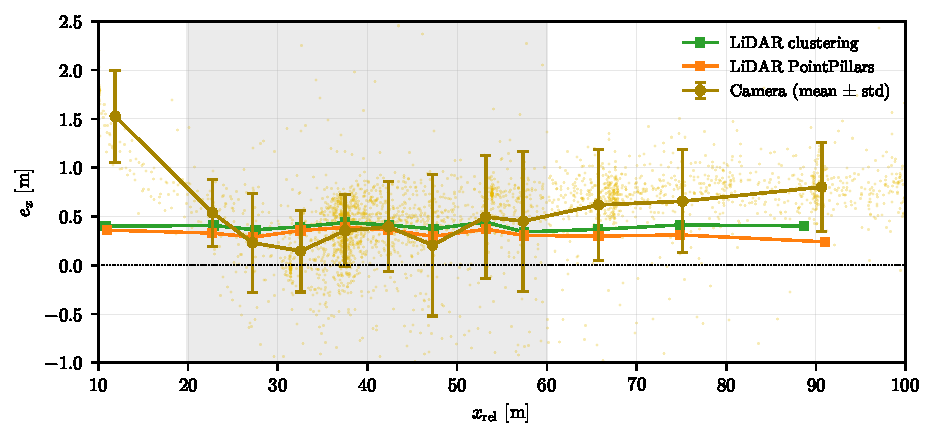
\includegraphics[width=\textwidth]{figures/ch4/det_cam_range.pdf}
    \caption[Longitudinal error of the camera as a function of $x_{\mathrm{rel}}$]{Longitudinal error of the camera as a function of $x_{\mathrm{rel}}$ in session
    07/26\_TUM, compared with the LiDARs. The shaded area is the operating range.}
    \label{fig:det_cam}
\end{figure}

\begin{table}[H]
    \centering
    \small
    \setlength{\tabcolsep}{6pt}
    \begin{tabular}{lcccc}
        \toprule
        & \multicolumn{2}{c}{Session 07/26\_TUM} & \multicolumn{2}{c}{Session 08/03\_Kinetiz} \\
        \cmidrule(lr){2-3}\cmidrule(lr){4-5}
        Sensor             & Mean [m] & Std [m] & Mean [m] & Std [m] \\
        \midrule
        LiDAR Clustering   & $0.41$   & $0.17$  & $-0.03$  & $0.18$  \\
        LiDAR PointPillars & $0.36$   & $0.13$  & $-0.07$  & $0.16$  \\
        Camera             & $0.35$   & $0.51$  & $-0.05$  & $0.37$  \\
        \bottomrule
    \end{tabular}
    \caption{Longitudinal error in the range 20--\SI{60}{m}.}
    \label{tab:det_long}
\end{table}



\subsection{Lateral Component}
\label{subsec:det_lat}

 Fig.~\ref{fig:det_lat} shows the lateral error of the LiDARs as a function of the
longitudinal position $x_{\mathrm{rel}}$ of the opponent, for session 07/26\_TUM. The
error shows a clear linear dependence on $x_{\mathrm{rel}}$. For this reason, the errors
are fitted with a straight line,
\begin{equation}
    e_y = a\,x_{\mathrm{rel}} + b,
    \label{eq:det_lat_fit}
\end{equation}
whose slope $a$ is estimated through a least squares fit on the data. The fit gives a
slope of \SI{0.60}{cm/m} for Clustering and \SI{0.58}{cm/m} for PointPillars. 

\begin{figure}[H]
    \centering
    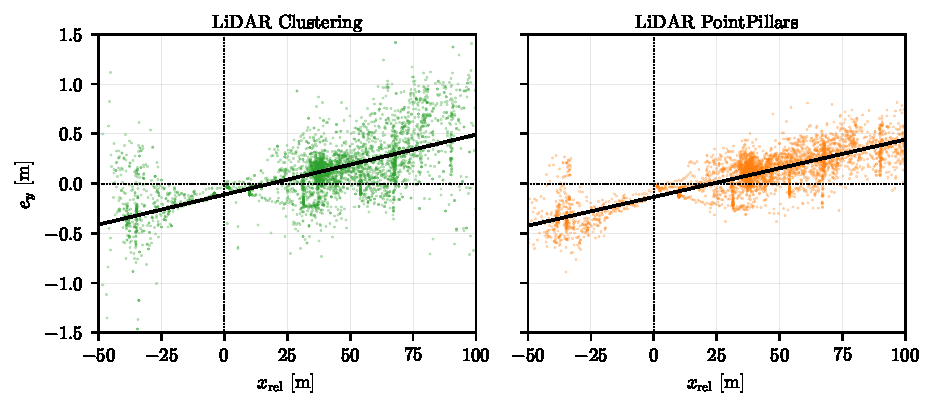
\includegraphics[width=\textwidth]{figures/ch4/det_lat_xrel.pdf}
    \caption[Lateral error of the LiDARs as a function of $x_{\mathrm{rel}}$]{Lateral error
    of the LiDARs as a function of $x_{\mathrm{rel}}$ in session 07/26\_TUM, with the least
    squares fit: slope of \SI{0.60}{cm/m} for Clustering and \SI{0.58}{cm/m} for
    PointPillars.}
    \label{fig:det_lat}
\end{figure}

The same analysis on session 08/03\_Kinetiz gives a slope of \SI{0.56}{cm/m} for
Clustering and \SI{0.52}{cm/m} for PointPillars, very close to the ones of the first
session. Interestingly, this behavior does not generalize to the other sensors. The slope
of the RaDAR is close to zero in both sessions, while the one of the camera changes from
\SI{1.23}{cm/m} in session 07/26\_TUM to \SI{-0.26}{cm/m} in session 08/03\_Kinetiz.

The fact that the trend is repeatable across the two datasets but observed only on the
LiDARs points to a cause related to the sensors rather than to the reference. The trend
is compatible with a small calibration offset of about \SI{0.33}{\degree} in yaw, since
a rotation $\delta\psi$ of the measured positions produces a lateral error
$e_y \simeq \delta\psi\,x_{\mathrm{rel}}$, exactly as observed. 

In the sessions at Yas Marina,  the behavior has been corrected, as shown in
Fig.~\ref{fig:det_lat_yas}, confirming that it was a matter of calibration.
\begin{figure}[H]
    \centering
    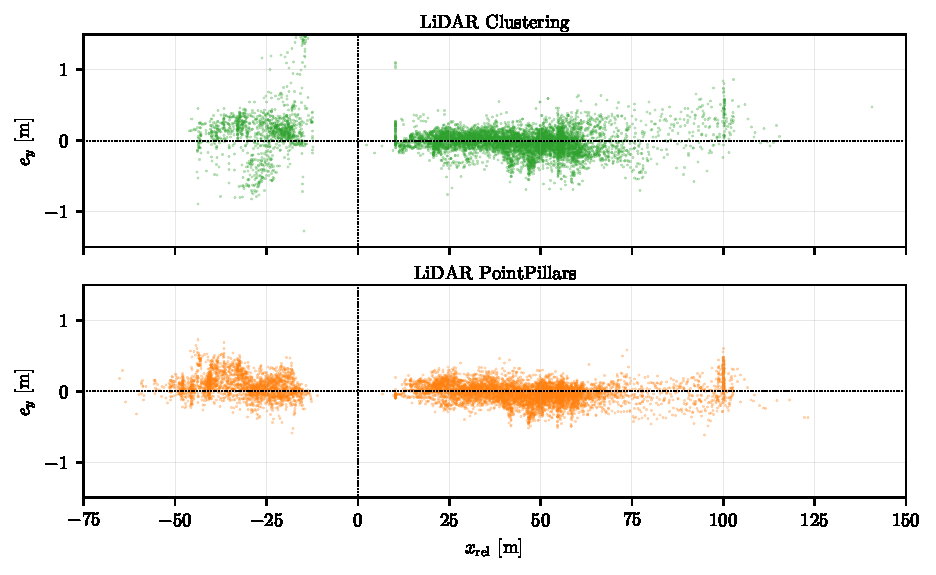
\includegraphics[width=\textwidth]{figures/ch4/det_lat_yas.pdf}
    \caption[Lateral error of the LiDARs after the recalibration]{Lateral error of the LiDARs
    as a function of $x_{\mathrm{rel}}$ in session 10/14\_eva, after the recalibration.}
    \label{fig:det_lat_yas}
\end{figure}

\FloatBarrier
% =====================================================================
\section{Global Error Trends of the Sensors}
\label{sec:macro}

Once the setup-related errors have been compensated, the errors related to the working
principle of each sensor and of its detection pipeline are analyzed, looking for the
trends that repeat across the sessions. The
analysis is organized by sensor. The two LiDAR pipelines are analyzed together, since
they process the same point clouds, while the RaDAR and the camera are treated separately.

\subsection{LiDAR}
\label{subsec:macro_lidar}

The errors of the two LiDAR pipelines are analyzed after the removal of the setup-related
errors identified in Section~\ref{sec:deterministic}.
Fig.~\ref{fig:lidar_clust_err} and Fig.~\ref{fig:lidar_pp_err} show the errors of
Clustering and PointPillars, together with their mean and standard deviation in intervals
of \SI{10}{m}.

The errors of Clustering remain centered on zero, but their spread grows with the range.
With the opponent ahead, the standard deviation of the lateral error increases from
0.11--\SI{0.18}{m} to 0.39--\SI{0.48}{m}, and the one of the longitudinal error from
0.13--\SI{0.17}{m} to 0.21--\SI{0.28}{m}. With the opponent behind, the standard deviation
at short range is comparable to the one observed with the opponent ahead; as the range
increases, however, the opponent enters the blind spot of the rear wing, and beyond
\SI{30}{m} the standard deviation reaches 0.33--\SI{0.62}{m} on both components. In both
cases, whether the opponent is farther or partially occluded, the growth of the standard
deviation is due to the reduced number of points returned by the sensor, which makes the
detections more unstable.

\begin{figure}[H]
    \centering
    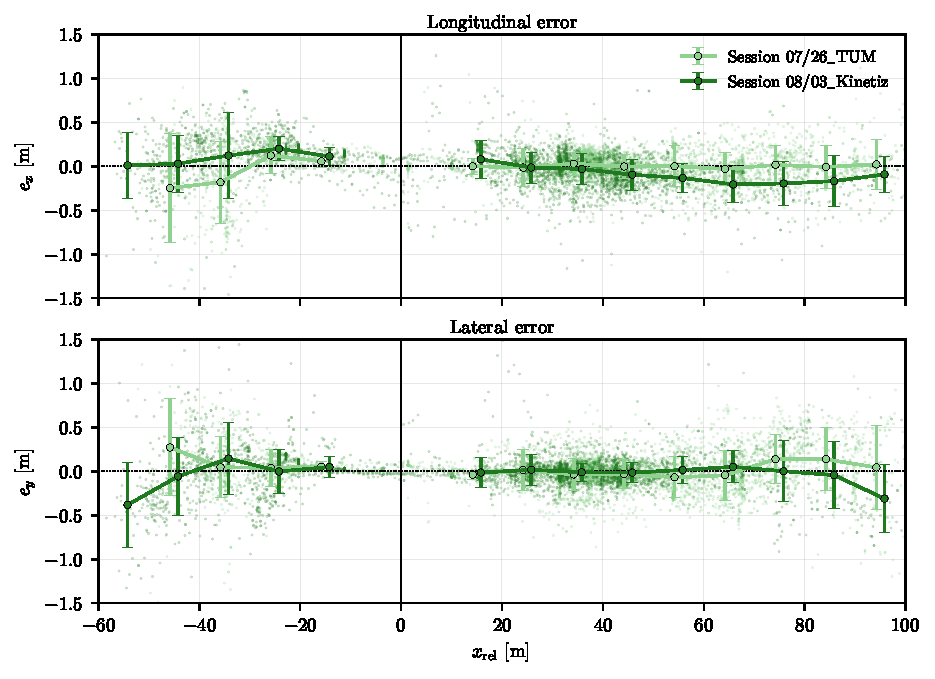
\includegraphics[width=\textwidth]{figures/ch4/lidar_clustering_errors.pdf}
    \caption{Longitudinal and lateral errors of LiDAR Clustering as a function of
    $x_{\mathrm{rel}}$, with mean and standard deviation in intervals of \SI{10}{m}.}
    \label{fig:lidar_clust_err}
\end{figure}

For PointPillars, the dependence on the range and on the occlusions manifests itself in a
different way. The standard deviation of its errors remains almost constant, below
\SI{0.2}{m}, and the detections are more stable. Since the bounding box is reconstructed
by a neural network, the opponent is identified consistently even when it is farther or
only partially visible. What degrades is instead the reconstruction of the depth. The
returned points lie only on the surfaces of the opponent facing the sensor, and the fewer
they are, the more the bounding box collapses towards them. With the opponent behind, the shift is about \SI{0.25}{m} in session
07/26\_TUM and \SI{0.18}{m} in session 08/03\_Kinetiz, while with the opponent ahead it
grows with the range, with a slope of \SI{0.17}{cm/m} and \SI{0.32}{cm/m} respectively. Overall, PointPillars
tends to produce detections shifted towards the ego vehicle.

\begin{figure}[H]
    \centering
    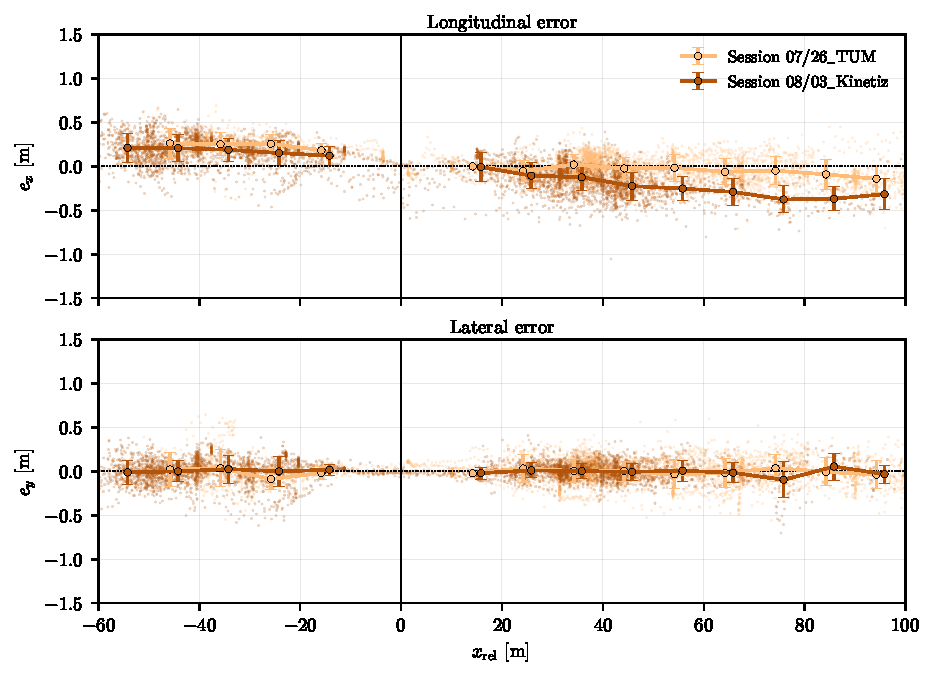
\includegraphics[width=\textwidth]{figures/ch4/lidar_pointpillars_errors.pdf}
    \caption{Longitudinal and lateral errors of LiDAR PointPillars as a function of
    $x_{\mathrm{rel}}$, with mean and standard deviation in intervals of \SI{10}{m}.}
    \label{fig:lidar_pp_err}
\end{figure}

The trends identified at Imola are validated on the sessions recorded at Yas Marina, whose
statistics are reported in Appendix~\ref{app:lidar}. The effect of the blind spot is most evident in session 10/14\_eva. In the other sessions
the opponent follows with a lateral offset of about \SI{6}{m}, while here, at short range,
it is almost aligned with the longitudinal axis of the ego vehicle, with a median
$|y_{\mathrm{rel}}| \approx \SI{2}{m}$. Including the samples with
$|y_{\mathrm{rel}}| < \SI{2}{m}$, the standard deviation of Clustering in the 10--\SI{20}{m}
interval behind reaches \SI{0.54}{m} longitudinally and \SI{0.58}{m} laterally, while
excluding them it drops to \SI{0.14}{m} and \SI{0.24}{m}, comparable to the values of the
other sessions.

Overall, the analysis shows that both Clustering and PointPillars are accurate and precise
when the opponent is ahead. Their reliability decreases when the opponent is behind, and
in these cases they need to be complemented with other sensors, i.e.\ the RaDAR.

Fig.~\ref{fig:lidar_blindspot} shows how Clustering and PointPillars detect the opponent
when it is behind the ego vehicle. PointPillars detects it more consistently but, as
anticipated, its measurement is displaced by an offset.

\begin{figure}[H]
    \centering
    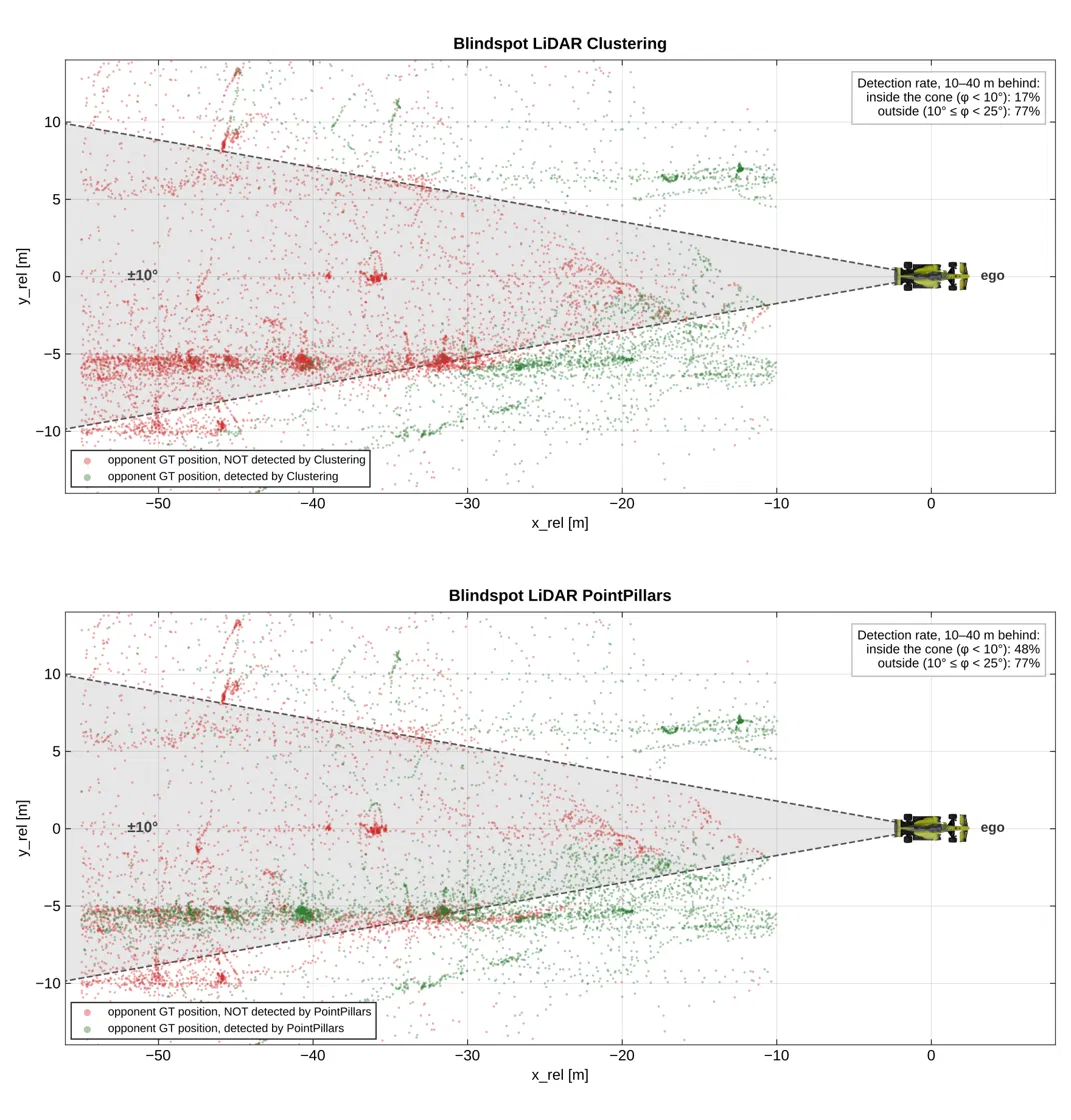
\includegraphics[width=\textwidth]{figures/ch4/lidar_blindspot.png}
    \caption{Blind spot of the LiDARs behind the ego vehicle. Positions of the opponent
    detected and not detected by Clustering (top) and PointPillars (bottom).}
    \label{fig:lidar_blindspot}
\end{figure}

\subsection{RaDAR}
\label{subsec:macro_radar}

The longitudinal error of the RaDAR is analyzed in the same way, separately for each
session. Fig.~\ref{fig:radar_long} shows the error as a function of the longitudinal
position of the opponent.

\begin{figure}[H]
    \centering
    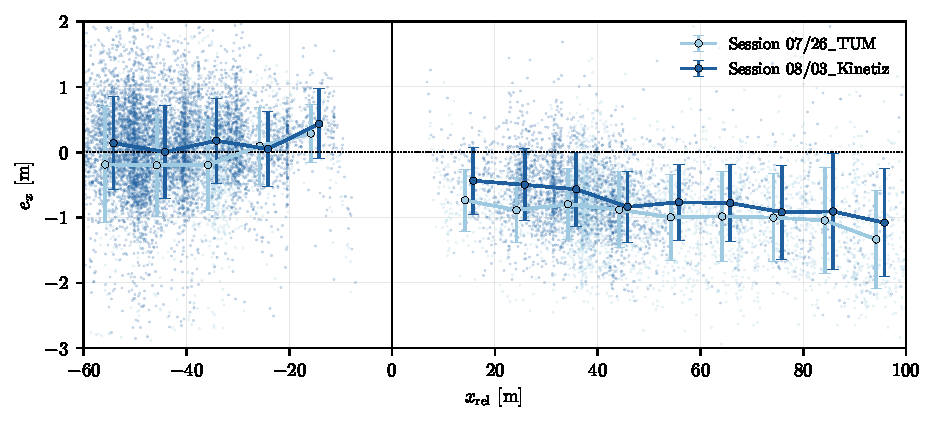
\includegraphics[width=\textwidth]{figures/ch4/radar_longitudinal_errors.pdf}
    \caption{Longitudinal error of the RaDAR as a function of $x_{\mathrm{rel}}$, with mean
    and standard deviation in intervals of \SI{10}{m}.}
    \label{fig:radar_long}
\end{figure}

Compared with the LiDARs, the RaDAR detections are much sparser. Already
at short range, the standard deviation of the longitudinal error is 0.42--\SI{0.51}{m},
three to four times the one of the LiDARs, and it tends to increase with the range,
although not monotonically, reaching 0.83--\SI{1.12}{m} behind and 0.71--\SI{0.82}{m}
ahead at 90--\SI{100}{m}.

The mean error is also different with the opponent ahead and behind, which results in two
different longitudinal offsets. With the opponent ahead, the detection is closer to the
ego vehicle than the ground truth, and the magnitude of the error grows with the range,
from \SI{-0.66}{m} in session 07/26\_TUM and \SI{-0.44}{m} in session 08/03\_Kinetiz at
10--\SI{20}{m} to \SI{-1.36}{m} and \SI{-1.06}{m} at 90--\SI{100}{m}. With the opponent
behind, instead, the mean error is small, mostly within $\pm\SI{0.25}{m}$ beyond
\SI{20}{m}.

Both behaviors are related to the working principle of the sensor. The angular resolution
of the RaDAR is much coarser than the one of the LiDARs, so the opponent is sampled with
only a few reflection points. The detection is the centroid of the cluster of these
points, and since their number and their distribution on the opponent change from one
cycle to the next, the centroid fluctuates significantly around the position of the
vehicle. This effect becomes more evident as the range increases, since the opponent
returns even fewer reflections.

The reflections also depend strongly on the surfaces of the opponent that face the sensor,
which further increases the variability of the detections. On the mean error, this
dependence produces the two different offsets, since the RaDAR observes two different
parts of the vehicle with the opponent ahead and behind, and the centroid is not
compensated with respect to the observed side. With the opponent ahead, most of the radar
waves are reflected by the rear wing, a large surface at the rear end of the car and the
closest to the sensor, so the detection is shifted towards the ego vehicle. With the
opponent behind, the RaDAR observes its front, i.e.\ the nose, the front wing, the wheels
and the sidepods, a reflecting surface distributed along the vehicle. The centroid of the
cluster is then closer to the center of the vehicle, and the offset is smaller. Both the
growth of the standard deviation and the two different offsets are validated on the
sessions recorded at Yas Marina, as reported in Appendix~\ref{app:lidar}.

Nevertheless, the rear RaDAR remains the only sensor that ensures the detection of the
opponent behind up to \SI{150}{m}, covering the range that the LiDARs cannot reach.

\subsection{Camera}
\label{subsec:macro_camera}

For the cameras, only data with the opponent ahead are available. Fig.~\ref{fig:camera_long}
shows the longitudinal error
as a function of the longitudinal position of the opponent, separately for each session.

\begin{figure}[H]
    \centering
    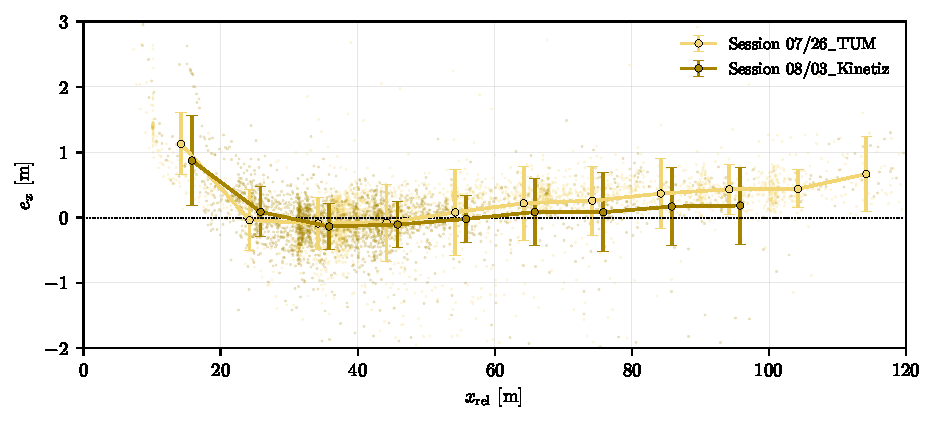
\includegraphics[width=\textwidth]{figures/ch4/camera_longitudinal_errors.pdf}
    \caption{Longitudinal error of the camera as a function of $x_{\mathrm{rel}}$, with mean
    and standard deviation in intervals of \SI{10}{m}.}
    \label{fig:camera_long}
\end{figure}

The dependence of the camera on the range appears mainly in the
mean of the longitudinal error, which follows a U-shaped trend. At short range, below
\SI{20}{m}, the detection is farther than the ground truth by about \SI{0.6}{m}. Between
20 and \SI{60}{m}, i.e.\ in the operating range identified in
Section~\ref{subsec:det_long}, the mean error is close to zero, within
$\pm\SI{0.1}{m}$, and the bias of the camera is comparable to the one of the LiDARs. Beyond this range, it increases again with the range and reaches
0.25--\SI{0.40}{m} at 90--\SI{100}{m}. A linear fit of the error beyond \SI{40}{m} gives a
slope of \SI{0.92}{cm/m} in session 07/26\_TUM and \SI{0.80}{cm/m} in session
08/03\_Kinetiz. The standard deviation
remains between 0.2 and \SI{0.5}{m}, without a clear trend with the range.

The growth of the error with the range is related to the way the camera estimates the
depth, which is obtained from the size of the bounding box in the image
(Section~\ref{sec:tt_perception}). As the opponent moves away, it spans fewer pixels and
its bounding box is estimated too small, so that the opponent is placed farther than it
actually is. The same trend is observed in the sessions recorded at Yas Marina, with slopes
between \SI{0.70}{cm/m} and \SI{1.48}{cm/m} beyond \SI{40}{m}, as reported in
Appendix~\ref{app:lidar}.

\FloatBarrier

% =====================================================================
\section{Gaussian Fit of the Residual Errors}
\label{sec:gaussian_fit}

Once the setup-related errors have been removed and the global trends of each sensor
have been characterized, the uncertainty of its measurements can be quantified and used to tune
the measurement noise covariance matrix $\mathbf{R}$ of the filter. This uncertainty is
expressed as a fixed standard deviation, obtained by fitting a Gaussian distribution to the
residual position errors. The fit is performed separately for the longitudinal and lateral
components and for the opponent ahead of and behind the ego vehicle. The errors are
computed as in Section~\ref{subsec:err_frames}.

All the sessions are considered together. The
detections with the ego vehicle moving slower than \SI{2}{m/s} are excluded.

Before the fit, the dependence of the mean error on the range, observed in
Section~\ref{sec:macro} for the camera and for PointPillars, is compensated. The errors are
grouped into intervals of \SI{10}{m} of $|x_{\mathrm{rel}}|$, and the median of each
interval is subtracted. The standard deviation of the Gaussian distribution is then
estimated as the sample standard deviation of the resulting residuals,
\begin{equation}
    \sigma = \sqrt{\frac{1}{N-1}\sum_{i=1}^{N}\left(r_i - \bar{r}\right)^2},
    \label{eq:sigma_std}
\end{equation}
where $r_i$ are the $N$ residuals and $\bar{r}$ their mean.

Table~\ref{tab:sensor_noise} reports the standard deviation of each sensor, while the
distributions of the residuals with the opponent ahead and behind, together with the
fitted Gaussian distributions, are shown in Fig.~\ref{fig:gauss68_front} and
Fig.~\ref{fig:gauss68_rear} in Appendix~\ref{app:lidar}. The LiDARs provide the most
accurate position measurement, with a standard deviation between \SI{0.11}{m} and
\SI{0.28}{m} on the longitudinal component and between \SI{0.14}{m} and \SI{0.33}{m} on
the lateral one, the largest values being those of Clustering with the opponent behind.
The camera has a standard deviation of \SI{0.38}{m} and \SI{0.43}{m}, while the RaDAR has
the largest longitudinal error, 0.68--\SI{0.76}{m}, and a lateral one of
0.32--\SI{0.39}{m}. Overall, the values identified are consistent with the analysis and the plots provided in the previous sections.

\begin{table}[H]
\centering
\small
\begin{tabular}{llcc}
\toprule
Sensor & Opponent & Longitudinal $\sigma_x$ [m] & Lateral $\sigma_y$ [m] \\
\midrule
LiDAR Clustering & Ahead & 0.15 & 0.20 \\
 & Behind & 0.28 & 0.33 \\
\midrule
LiDAR PointPillars & Ahead & 0.12 & 0.14 \\
 & Behind & 0.11 & 0.15 \\
\midrule
RaDAR & Ahead & 0.68 & 0.39 \\
 & Behind & 0.76 & 0.32 \\
\midrule
Camera & Ahead & 0.38 & 0.43 \\
\bottomrule
\end{tabular}
\caption{Standard deviation of the residual errors, all sessions pooled.}
\label{tab:sensor_noise}
\end{table}

It is important to point out that the resulting values describe the error of each sensor in the operating conditions in which
the data were collected. They do not correspond to the accuracy declared in the datasheets,
which refers to optimal conditions, and they would be different with a dataset of different
characteristics. With the median of the range shifted to longer distances, e.g.\
\SI{90}{m}, the standard deviation of the RaDAR and of LiDAR Clustering, which grows with
the range, would be larger. Since the purpose of the analysis is the tuning of
$\mathbf{R}$, i.e.\ weighting each sensor correctly in the filter, these values are
nevertheless the appropriate ones, as they reflect the errors expected in the nominal
operating conditions of the vehicle.


% =====================================================================
\section{Local Behavior of the Residual Errors}
\label{sec:gauss_markov}

The Kalman filter assumes that the measurement errors are white, i.e.\ uncorrelated
between different time instants. As introduced in Section~\ref{sec:tt_correction}, the
measurement noise is modeled as a zero-mean Gaussian white sequence,
\begin{equation}
    \mathbb{E}\left[\mathbf{v}_k\,\mathbf{v}_j^\top\right] = \mathbf{R}_k\,\delta_{kj}.
    \label{eq:white_noise}
\end{equation}
The residual errors obtained after the removal of the trends shown in the previous
sections, however, still contain a local autocorrelated component, which contrasts with
this assumption. The purpose of this section is to analyze this component, to model it
and to compensate for it.

\subsection{Autocorrelation and Power Spectral Density}
\label{subsec:acf_psd}

The local component is analyzed in the frequency domain, through the power spectral
density (PSD) of the residual errors, and in the time domain, through their
autocorrelation. Since the opponent is not always detected, the residuals of each sensor
are first split into continuous segments, interrupted wherever two consecutive detections
are more than \SI{0.55}{s} apart, each resampled on a uniform grid with the sampling
period of the sensor and with its mean removed. The PSD $S_e(f)$ of each segment is
estimated with the Welch method, with a Hann window of 128 samples and \SI{50}{\percent}
overlap, and the spectra of all the segments are averaged. The
autocorrelation is then derived from the resulting PSD through the Wiener--Khinchin
theorem,
\begin{equation}
    R_e(\ell) = \int_{-\infty}^{+\infty} S_e(f)\, e^{\,j 2\pi f \ell}\, df,
    \qquad
    \rho_e(\ell) = \frac{R_e(\ell)}{R_e(0)},
    \label{eq:wiener_khinchin}
\end{equation}
where $\ell$ is the time lag and $\rho_e$ the normalized autocorrelation.

For sessions 07/26\_TUM and 10/14\_eva, with the opponent ahead, the PSD and the
autocorrelation of the residual errors are shown in Fig.~\ref{fig:psd_acf} and summarized
in Tables~\ref{tab:psd_sessions} and~\ref{tab:acf_sessions}. The PSD of the LiDARs and of
the camera concentrate most of the power at low frequency, between about 60 and
\SI{90}{\percent} below \SI{2}{Hz}, where they decrease approximately as $1/f^2$, and
show a white floor beyond \SI{2}{Hz}. In the time domain, the autocorrelation decays
gradually, is still between about 0.25 and 0.55 at \SI{0.5}{s} and vanishes only after
1--\SI{2}{s}, so that the errors of consecutive detections are strongly correlated. The
RaDAR has the highest PSD, consistent with its larger error, but the flattest spectrum,
and its autocorrelation drops below 0.3 at \SI{0.5}{s}, i.e.\ its error is closer to a
white sequence.

\begin{figure}[H]
    \centering
    \subfloat[PSD]{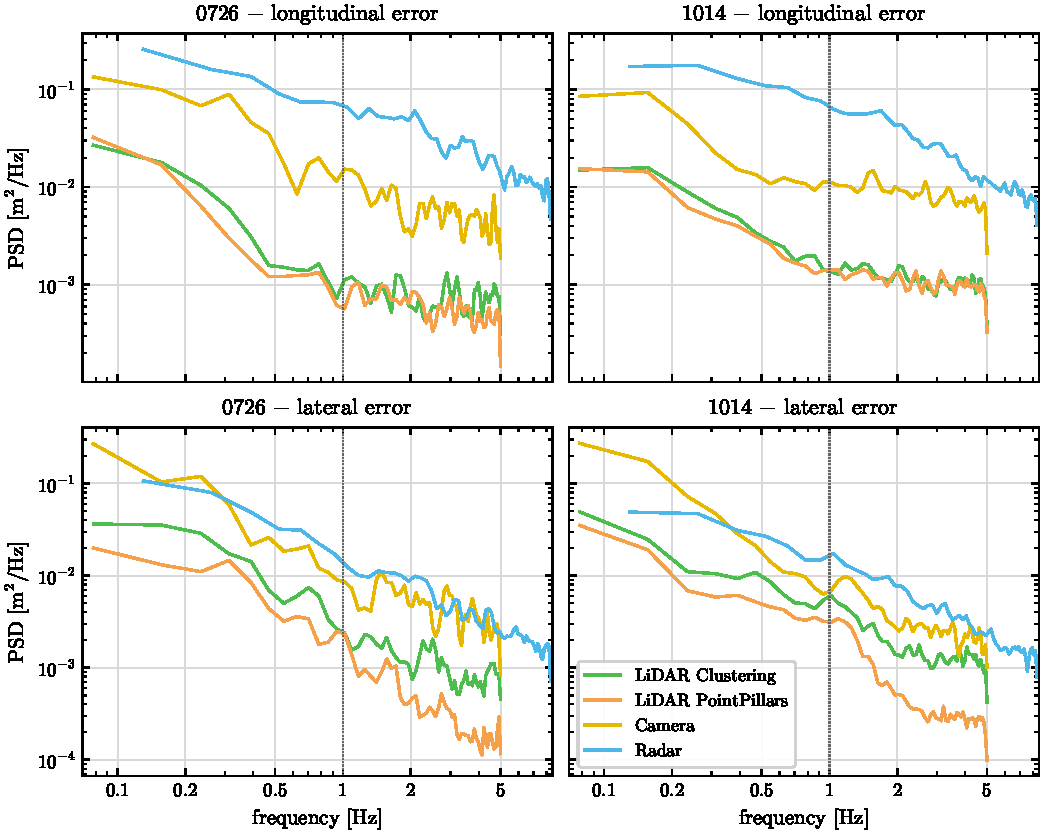
\includegraphics[width=0.49\textwidth]{figures/ch4/error_psd.pdf}}
    \hfill
    \subfloat[Autocorrelation]{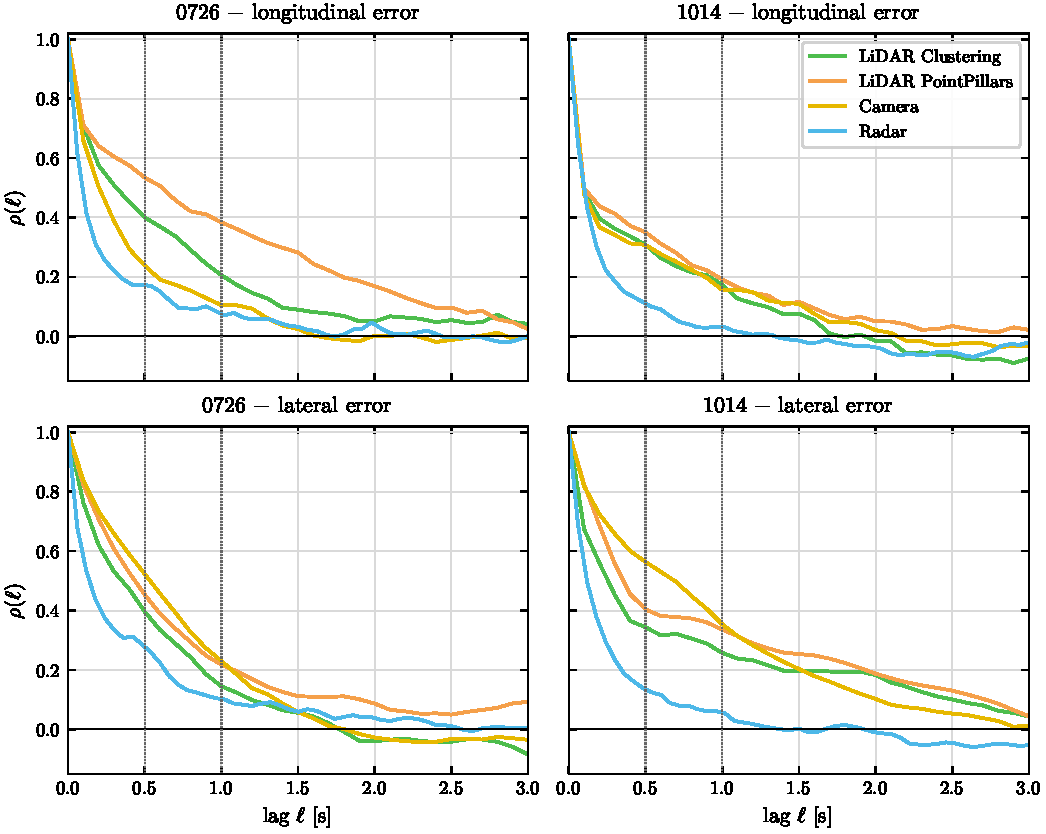
\includegraphics[width=0.49\textwidth]{figures/ch4/error_acf.pdf}}
    \caption{PSD and autocorrelation of the residual errors, opponent ahead, sessions
    07/26\_TUM and 10/14\_eva.}
    \label{fig:psd_acf}
\end{figure}

\begin{table}[H]
\centering
\small
\setlength{\tabcolsep}{4pt}
\begin{tabular}{llcccc}
\toprule
 & & \multicolumn{2}{c}{$P_{<1\,\mathrm{Hz}}$ [\%]} & \multicolumn{2}{c}{$P_{<2\,\mathrm{Hz}}$ [\%]} \\
\cmidrule(lr){3-4}\cmidrule(lr){5-6}
Sensor & Axis & 07/26 & 10/14 & 07/26 & 10/14 \\
\midrule
LiDAR Clustering & Long. & 65 & 53 & 76 & 67 \\
 & Lat. & 74 & 63 & 84 & 80 \\
\midrule
LiDAR PointPillars & Long. & 69 & 52 & 80 & 66 \\
 & Lat. & 80 & 75 & 91 & 91 \\
\midrule
Camera & Long. & 65 & 44 & 78 & 62 \\
 & Lat. & 74 & 80 & 84 & 89 \\
\midrule
RaDAR & Long. & 45 & 48 & 68 & 72 \\
 & Lat. & 64 & 53 & 80 & 76 \\
\bottomrule
\end{tabular}
\caption{Fraction of the power of the residual errors below 1 and \SI{2}{Hz}.}
\label{tab:psd_sessions}
\end{table}

\begin{table}[H]
\centering
\small
\setlength{\tabcolsep}{4pt}
\begin{tabular}{llcccccccc}
\toprule
 & & \multicolumn{2}{c}{$\ell=\SI{0.2}{s}$} & \multicolumn{2}{c}{$\ell=\SI{0.5}{s}$} & \multicolumn{2}{c}{$\ell=\SI{1}{s}$} & \multicolumn{2}{c}{$\ell=\SI{2}{s}$} \\
\cmidrule(lr){3-4}\cmidrule(lr){5-6}\cmidrule(lr){7-8}\cmidrule(lr){9-10}
Sensor & Axis & 07/26 & 10/14 & 07/26 & 10/14 & 07/26 & 10/14 & 07/26 & 10/14 \\
\midrule
LiDAR Clustering & Long. & 0.58 & 0.40 & 0.40 & 0.31 & 0.21 & 0.17 & 0.05 & $-$0.02 \\
 & Lat. & 0.62 & 0.56 & 0.40 & 0.34 & 0.14 & 0.26 & $-$0.04 & 0.18 \\
\midrule
LiDAR PointPillars & Long. & 0.64 & 0.44 & 0.53 & 0.35 & 0.38 & 0.19 & 0.17 & 0.05 \\
 & Lat. & 0.71 & 0.69 & 0.45 & 0.40 & 0.22 & 0.34 & 0.09 & 0.19 \\
\midrule
Camera & Long. & 0.50 & 0.37 & 0.24 & 0.31 & 0.10 & 0.16 & 0.00 & 0.02 \\
 & Lat. & 0.73 & 0.72 & 0.52 & 0.56 & 0.23 & 0.35 & $-$0.03 & 0.10 \\
\midrule
RaDAR & Long. & 0.29 & 0.28 & 0.17 & 0.11 & 0.08 & 0.03 & 0.05 & $-$0.04 \\
 & Lat. & 0.42 & 0.35 & 0.28 & 0.13 & 0.10 & 0.06 & 0.04 & $-$0.01 \\
\bottomrule
\end{tabular}
\caption{Normalized autocorrelation $\rho_e(\ell)$ of the residual errors, opponent ahead.}
\label{tab:acf_sessions}
\end{table}

The comparison between the two LiDAR pipelines gives an indication of the origin of this
component. Since Clustering and PointPillars process the same point clouds, their errors
at the same scan can be decomposed into a common mode and a differential mode,
\begin{equation}
    e_{\mathrm{c}} = \frac{e_{\mathrm{C}} + e_{\mathrm{PP}}}{2},
    \qquad
    e_{\mathrm{d}} = \frac{e_{\mathrm{C}} - e_{\mathrm{PP}}}{2},
    \label{eq:common_mode}
\end{equation}
where $e_{\mathrm{C}}$ and $e_{\mathrm{PP}}$ are the errors of Clustering and
PointPillars. Most of the low-frequency content is found in the common mode, i.e.\ the
slow component is largely shared by the two pipelines. Its source is therefore not only
the detection pipeline of each sensor, but also the way in which the point cloud is
sampled and built. Since this component evolves slowly and affects both pipelines in the
same way, it suggests a dependence on the relative geometry or on the relative kinematics
of the two vehicles, which also vary slowly and determine how the opponent is sampled by
the sensor.

\subsection{Correlation with the Geometry}
\label{subsec:corr_geometry}

\TODO{Cross-correlation of the residuals with range, $y_{\mathrm{rel}}$, relative yaw:
how much of the temporal correlation is explained by the slowly varying geometry.}

\subsection{Gauss-Markov Model}
\label{subsec:gauss_markov_model}

Having excluded a dependence on the geometry, the low-frequency component is compensated
by estimating it and removing it from the error, which isolates the white part. The error
of each sensor and component is therefore modeled as the sum of an autocorrelated term
$b_k$ and of a white term $w_k$,
\begin{equation}
    e_k = b_k + w_k,
    \qquad
    w_k \sim \mathcal{N}\!\left(0,\, \sigma_w^2\right),
    \label{eq:gm_decomposition}
\end{equation}
where $b_k$ is a first-order Gauss-Markov process,
\begin{equation}
    b_{k+1} = \phi\, b_k + \eta_k,
    \qquad
    \phi = e^{-\Delta t/\tau},
    \qquad
    \eta_k \sim \mathcal{N}\!\left(0,\, \sigma_b^2\,(1-\phi^2)\right),
    \label{eq:gm_process}
\end{equation}
with $\Delta t$ the sampling period and $\tau$ the correlation time. The variance of
$\eta_k$ keeps the variance of $b_k$ equal to $\sigma_b^2$, so that the variance of the
error is $\sigma_b^2 + \sigma_w^2$. Based on the PSD and on the autocorrelation, $\tau$ is
set to \SI{1}{s} for all the sensors, for simplicity.

Since $w_k$ is uncorrelated between consecutive samples, the covariance of two
consecutive errors depends only on $b_k$. Following~\eqref{eq:gm_process}, $\sigma_b^2$ is
estimated by least squares on the pairs of consecutive detections, and $\sigma_w^2$ is
obtained by difference,
\begin{equation}
    \mathbb{E}\left[e_k\, e_{k+1}\right] = \phi_k\, \sigma_b^2
    \;\Rightarrow\;
    \hat{\sigma}_b^2 = \frac{\sum_k \phi_k\, e_k\, e_{k+1}}{\sum_k \phi_k^2},
    \qquad
    \hat{\sigma}_w^2 = \mathrm{Var}(e) - \hat{\sigma}_b^2,
    \label{eq:gm_sigmas}
\end{equation}
where $\phi_k$ is computed with the actual time between the two detections.

\begin{table}[H]
\centering
\small
\setlength{\tabcolsep}{4pt}
\begin{tabular}{llcccc}
\toprule
 & & \multicolumn{2}{c}{$\sigma_b$ [m]} & \multicolumn{2}{c}{$\sigma_w$ [m]} \\
\cmidrule(lr){3-4}\cmidrule(lr){5-6}
Sensor & Axis & 07/26 & 10/14 & 07/26 & 10/14 \\
\midrule
LiDAR Clustering & Long. & 0.15 & 0.09 & 0.09 & 0.08 \\
 & Lat. & 0.21 & 0.13 & 0.12 & 0.08 \\
\midrule
LiDAR PointPillars & Long. & 0.13 & 0.08 & 0.05 & 0.07 \\
 & Lat. & 0.14 & 0.12 & 0.05 & 0.04 \\
\midrule
Camera & Long. & 0.40 & 0.21 & 0.34 & 0.21 \\
 & Lat. & 0.53 & 0.30 & 0.24 & 0.12 \\
\midrule
RaDAR & Long. & 0.45 & 0.30 & 0.53 & 0.51 \\
 & Lat. & 0.35 & 0.17 & 0.32 & 0.22 \\
\bottomrule
\end{tabular}
\caption{Standard deviations of the autocorrelated and white components of the residual
errors, opponent ahead, $\tau = \SI{1}{s}$.}
\label{tab:gm_sigmas}
\end{table}

Table~\ref{tab:gm_sigmas} reports $\sigma_b$ and $\sigma_w$. For the LiDARs and the
camera $\sigma_b$ is larger than $\sigma_w$, i.e.\ most of the error is autocorrelated,
while for the RaDAR the white term is comparable to or larger than the autocorrelated
one, consistently with its faster decorrelation. The same split is found in all the
sessions. Once the estimated $b_k$ is removed from the error, the residuals are correctly
decorrelated, and their autocorrelation drops to about zero at all the lags, as shown in
Table~\ref{tab:acf_gm}.

\begin{table}[H]
\centering
\small
\setlength{\tabcolsep}{4pt}
\begin{tabular}{llccc}
\toprule
Sensor & Axis & $\ell=\SI{0.2}{s}$ & $\ell=\SI{0.5}{s}$ & $\ell=\SI{1}{s}$ \\
\midrule
LiDAR Clustering & Long. & $-0.10$ to $+0.03$ & $-0.05$ to $+0.07$ & $-0.01$ to $+0.04$ \\
 & Lat. & $-0.06$ to $+0.03$ & $-0.06$ to $+0.00$ & $-0.09$ to $+0.06$ \\
\midrule
LiDAR PointPillars & Long. & $-0.15$ to $-0.01$ & $-0.08$ to $+0.03$ & $-0.02$ to $+0.06$ \\
 & Lat. & $-0.12$ to $+0.08$ & $-0.12$ to $+0.00$ & $-0.10$ to $+0.03$ \\
\midrule
Camera & Long. & $-0.09$ to $+0.07$ & $-0.08$ to $+0.09$ & $-0.03$ to $+0.09$ \\
 & Lat. & $-0.07$ to $+0.04$ & $-0.01$ to $+0.16$ & $-0.01$ to $+0.06$ \\
\midrule
RaDAR & Long. & $-0.08$ to $+0.01$ & $-0.08$ to $-0.02$ & $-0.06$ to $+0.07$ \\
 & Lat. & $-0.10$ to $+0.01$ & $-0.13$ to $+0.02$ & $-0.05$ to $+0.03$ \\
\bottomrule
\end{tabular}
\caption{Normalized autocorrelation of the residual errors after the removal of the
autocorrelated component, opponent ahead. Range across the sessions.}
\label{tab:acf_gm}
\end{table}

\subsection{Low-Frequency Bias of the LiDARs}
\label{subsec:lidar_lf_bias}

\TODO{Not observable without an absolute reference, followed by the track. Effect on the
innovations of camera and RaDAR, relative bias states with the LiDAR as reference.}

% =====================================================================
\section{Adaptive Measurement Noise Covariance}
\label{sec:adaptive_r}

\TODO{Covariance matching on the decorrelated innovations, window length related to
$\tau$, $\sigma$ of Section~\ref{sec:gaussian_fit} as nominal value.}

% =====================================================================
\section{Results}
\label{sec:ch4_results}

\TODO{Fixed $\mathbf{R}$ and adaptive $\mathbf{R}$. NEES/NIS with $\chi^2$ bounds, RMSE ahead/behind and per range, critical
episodes, adaptive $\mathbf{R}$ vs $\sigma$(range), whiteness of the normalized
innovations.}

\chapter{Q Feed-Forward}
\label{ch:qff}

The motion model of the tracker, introduced in Section~\ref{subsec:tt_cca}, assumes that
the opponent moves with constant curvature and constant longitudinal acceleration over
each prediction interval. This assumption holds well when the dynamics of the opponent
changes slowly, e.g.\ on a straight or in the middle of a corner, but it is violated at
the beginning and at the end of the maneuvers. When the opponent starts braking, or
passes from braking to traction, the acceleration changes abruptly, and the actual
motion departs from the one predicted by the CCA model. In these conditions, the dynamic
model is no longer correct and the quality of the estimate degrades. The filter relies on
the motion model more than it should, and it follows the new dynamics only after several
measurements have confirmed it, so that the estimate lags behind the true state of the
opponent.

This behavior is shown in Fig.~\ref{fig:qff_cca_baseline}, which compares the speed and the
acceleration estimated by the filter with the CCA model and the nominal process noise with the
ground truth over two braking maneuvers. At the onset of each braking, the estimated
acceleration departs from the ground truth with a delay of several tenths of a second, and the
lag accumulated in this interval is reflected on the speed, which is overestimated during the
braking and underestimated at its end.

\begin{figure}[H]
    \centering
    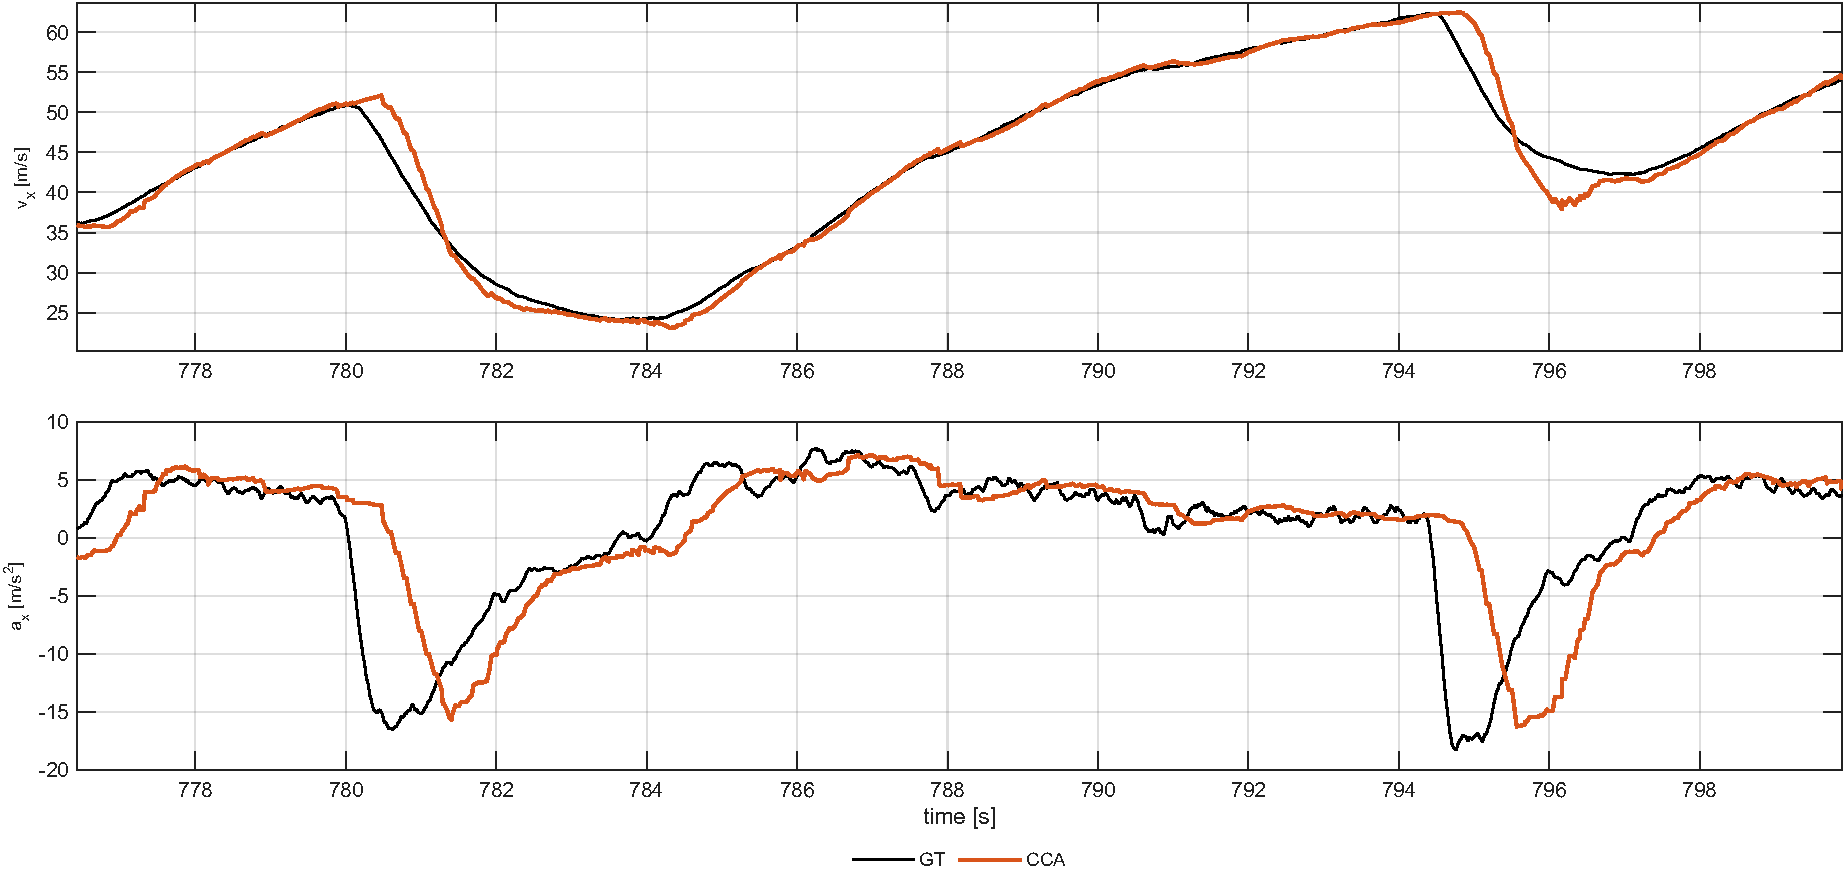
\includegraphics[width=0.8\textwidth]{figures/ch5/cca_baseline.pdf}
    \caption{Speed and acceleration estimated with the CCA model and the nominal process
    noise. Session of 5 September 2026, Imola.}
    \label{fig:qff_cca_baseline}
\end{figure}

Several approaches have been proposed to adapt a filter to the maneuvers of a target. A
first family adapts the process noise online from the innovations of the filter, as in the
covariance matching techniques, which estimate $\mathbf{Q}$ recursively from the discrepancy between the observed and the predicted dispersion of the
innovations, without requiring an explicit description of the maneuver. A second line of
research comprises the multiple model approaches, which estimate the state through several
filters running in parallel, each based on a motion model representative of an operating
condition of the vehicle. In the classical multiple model formulation, the filters evolve
independently and their estimates are only combined at the output, weighted by model
probabilities computed from the likelihood of the innovations. In the Interacting Multiple
Model (IMM) filter, instead, the filters also interact, since at each step their initial
conditions are obtained by mixing the estimates of all the models according to the
transition probabilities between them, which allows the estimate to follow the switches
between the operating conditions of the vehicle. These approaches describe the different
phases of the race with dedicated models, at the cost of a higher computational load, of a
larger number of parameters to tune, such as the transition probabilities between the
models, and of the need to mix states of different dimension. A further line, to which the
approach presented in this chapter belongs, is based on a maneuver detection logic, and it
lies between the previous two, since it starts from a single motion model but switches
between two distinct behaviors of the filter, with a nominal and an inflated process noise,
according to an explicit detection of the maneuver.

To recover the quality of the estimate during the maneuvers, a feed-forward approach on
the process noise covariance is therefore implemented. Its idea and rationale are explained in
Section~\ref{sec:qff_idea}, and Section~\ref{sec:qff_nominal} describes the preliminary tuning
of the nominal process noise, which is the starting value of the method.
Section~\ref{sec:qff_formulation} presents the feed-forward formulation, together with the
maneuver detection logic based on the jerk of the opponent and its implementation in the
tracker. Finally, Section~\ref{sec:qff_results} compares the resulting estimate with the one of
the nominal filter.

% =====================================================================
\section{The Idea}
\label{sec:qff_idea}

The idea behind the feed-forward approach presented in this chapter starts from how the
process noise covariance $\mathbf{Q}_k$ influences the gain of the Kalman filter. The
process noise represents the uncertainty of the motion model, i.e.\ how much the actual
motion of the opponent is expected to differ from the predicted one. In the prediction
step, it is added to the covariance propagated through the motion model,
\begin{equation}
    \mathbf{P}_{k+1|k} = \mathbf{F}_k\,\mathbf{P}_{k|k}\,\mathbf{F}_k^\top + \mathbf{Q}_k,
    \label{eq:qff_pred_cov}
\end{equation}
and the predicted covariance enters the Kalman gain of the correction step,
\begin{equation}
    \mathbf{K}_{k+1} = \mathbf{P}_{k+1|k}\,\mathbf{H}_{k+1}^\top
    \left(\mathbf{H}_{k+1}\,\mathbf{P}_{k+1|k}\,\mathbf{H}_{k+1}^\top + \mathbf{R}_{k+1}\right)^{-1},
    \label{eq:qff_gain}
\end{equation}
as in~\eqref{eq:tt_prediction} and~\eqref{eq:tt_update}. Considering a single component,
with a predicted variance $P$ and a measurement noise variance $R$, the gain reduces to
\begin{equation}
    K = \frac{P}{P + R},
    \label{eq:qff_gain_scalar}
\end{equation}
which ranges between zero, when the prediction is much more accurate than the
measurement, and one, when the measurement is much more accurate than the prediction.
Increasing $\mathbf{Q}_k$ increases $P$ and therefore $K$, so that the corrected state
moves away from the prediction and towards the measurement. Through the off-diagonal
terms of $\mathbf{P}_{k+1|k}$, the effect is not limited to the measured position. The
process noise of the CCA model acts on the acceleration and on the curvature
(Section~\ref{subsec:tt_cca}), and a larger uncertainty on these states allows the
correction of the position to be transferred more quickly to the speed and to the
acceleration, which are not measured directly by the LiDARs and by the camera.

By varying $\mathbf{Q}_k$, different behaviors of the filter are therefore obtained. A
large process noise leads to a large gain and therefore to a more reactive filter, which
follows the changes of the dynamics quickly but returns a noisy estimate. A small process
noise, instead, keeps the gain small, and the filter remains anchored to the prediction,
with a smoother estimate that is often delayed with respect to the true state.

\begin{figure}[H]
    \centering
    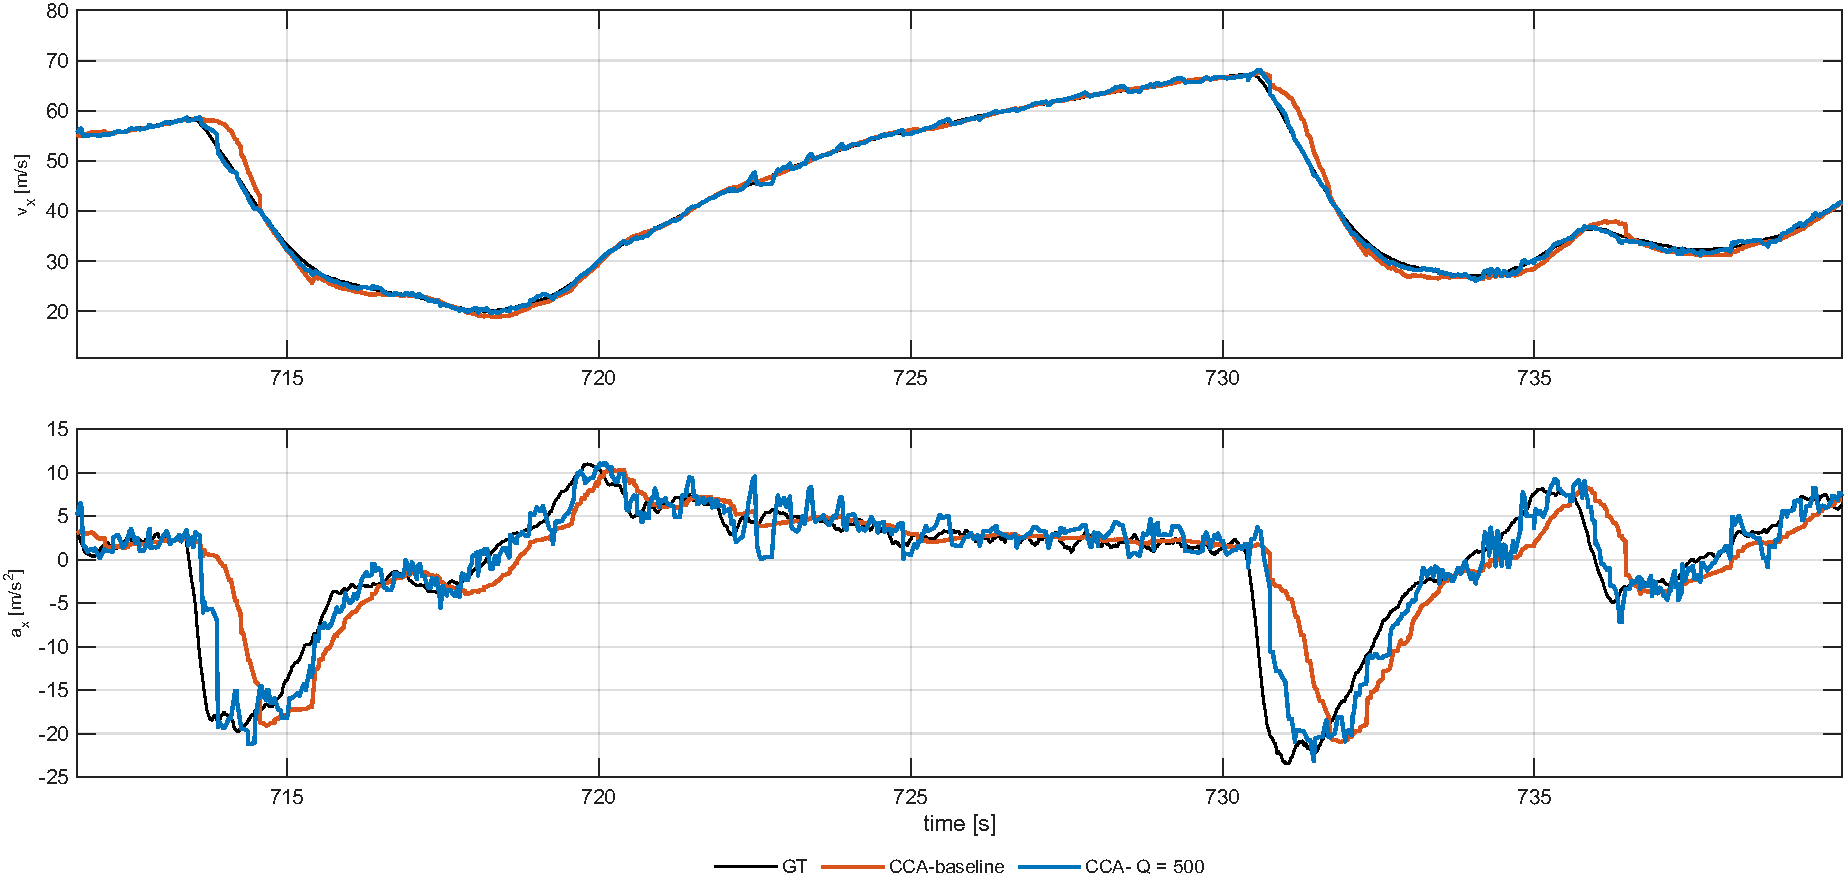
\includegraphics[width=\textwidth]{figures/ch5/q_high_vs_baseline.pdf}
    \caption{Speed and acceleration estimated with the nominal and with an increased process
    noise. Session of 5 September 2026, Imola.}
    \label{fig:qff_highq}
\end{figure}

Fig.~\ref{fig:qff_highq} shows the speed and the longitudinal acceleration of the opponent
estimated by the filter with the CCA model, with the nominal process noise and with an
increased one, obtained with $q_a = 500$, compared with the ground truth over two braking
maneuvers. The figure confirms the previous considerations. With the increased process noise,
the filter corrects the prediction more with the information of the measurements, and it is
therefore considerably more reactive at the changes of maneuver, with an acceleration that
closely follows the ground truth at the beginning and at the end of the braking phases. The
nominal filter, instead, follows the same transitions with a visible delay, which is also
reflected on the speed at the beginning of each braking.

Adopting the increased process noise over the whole lap, however, is not a correct solution,
since in the phases at constant acceleration the larger gain makes the filter follow the noise
of the measurements, and the estimate of the acceleration becomes noisier without any benefit,
as visible in Fig.~\ref{fig:qff_highq} between the two maneuvers. At the same time, a process
noise fixed at its nominal value cannot cover the whole spectrum of the dynamics of the
vehicle, which alternates slowly varying phases with abrupt transitions between traction and
braking. From these considerations arises the idea of the approach presented in this chapter,
i.e.\ to alternate between the two values of the process noise through a maneuver detection
logic, which in this work is implemented as a feed-forward approach and is presented in
Section~\ref{sec:qff_formulation}, after the tuning of the nominal process noise.

% =====================================================================
\section{Nominal Process Noise Tuning}
\label{sec:qff_nominal}

Preliminary to the feed-forward approach is the tuning of the nominal value
$\mathbf{Q}_{\mathrm{nom}}$ of the process noise, i.e.\ of the spectral densities $q_a$
and $q_\kappa$ of Section~\ref{subsec:tt_cca}. The choice is made by testing different
values of the process noise and selecting the one that gives a good starting point on the
trade-off introduced in the previous section, between the reactivity of the filter to
the changes of the dynamics and the noise of the estimate. This value is the baseline of
the feed-forward approach, in which it is multiplied by an inflation factor during the
maneuvers.

\TODO{Figures with the estimate obtained with different values of the process noise, and
their effect on the quality of the estimate.}

% =====================================================================
\section{Feed-Forward Formulation}
\label{sec:qff_formulation}

In the feed-forward formulation, the process noise covariance of the filter is switched
between two values, the nominal one, suited to the phases in which the dynamics of the
opponent changes slowly, and an inflated one, which makes the filter reactive during the
maneuvers. The switch is driven by a maneuver flag $f_k$, which is activated when a maneuver is
detected and deactivated when it is over,
\begin{equation}
    \mathbf{Q}_k =
    \begin{cases}
        \mathbf{Q}_{\mathrm{nom}} & \text{if } f_k = 0, \\
        \lambda\,\mathbf{Q}_{\mathrm{nom}} & \text{if } f_k = 1,
    \end{cases}
    \label{eq:qff_switch}
\end{equation}
where $\mathbf{Q}_{\mathrm{nom}}$ is the nominal process noise of
Section~\ref{sec:qff_nominal} and $\lambda > 1$ the inflation factor. The flag therefore
selects at each step which of the two behaviors of the filter is adopted, the reactive or the
nominal one, while the motion model and the structure of the filter remain unchanged.

The maneuver detection is based on the jerk of the opponent, i.e.\ the time derivative of its
longitudinal acceleration, which is the natural candidate for this purpose. The CCA model
assumes a constant acceleration over each prediction interval, and the jerk, being its
derivative, directly measures how much the actual motion departs from this assumption, so that
its magnitude is small in the phases that the model describes correctly and large at the
beginning and at the end of the maneuvers. The detection logic is described in
Section~\ref{subsec:qff_detection}, and its implementation in the tracker in
Section~\ref{subsec:qff_implementation}.

\subsection{Maneuver Detection Logic}
\label{subsec:qff_detection}

As anticipated in the previous section, the maneuver is detected from the instantaneous value
of the jerk of the opponent. Since the jerk is not measured by the sensors, it has to be
estimated, and two approaches are possible.

The first consists in augmenting the state of the filter with the jerk, which turns the CCA
model into a constant-jerk model, in which the jerk evolves as a random walk driven by a white
noise on its derivative. Besides requiring a new formulation of the motion model, of its
Jacobians and of the discretized process noise, whose terms would propagate to all the other
states, this solution is not pursued for two main reasons. The jerk would be observed only
indirectly, since it is separated by two integrations from the range rate of the RaDAR and by
three from the measured position, so that its estimate would be corrected only through the
cross-covariance terms of the filter, with a small gain and a convergence time comparable to
the duration of the maneuvers themselves, which contrasts with the need for an early
detection. Moreover, the additional state would modify the estimator published to the planning
module also where the CCA model is adequate, since a higher-order model amplifies the effect of
the measurement noise on the prediction, whereas the purpose of the detection is only to
select the process noise, leaving the nominal behavior of the filter unchanged outside the
maneuvers.

The second approach, adopted in this work, consists in obtaining the jerk by differentiating
and filtering the estimated acceleration. The filtering limits the amplification of the
high-frequency noise caused by the differentiation, and two families of filters are
considered, time-domain and frequency-based ones.

\paragraph{Time-domain filters.} In this family, the differentiated acceleration is
filtered by interpolating the signal with a polynomial of degree $n$ over a moving window
of $m$ samples. The degree of the polynomial sets the degrees of freedom of the fit,
while the length of the window sets the number of samples used for the fitting, and
therefore the amount of smoothing. The classical filter of this family is the
Savitzky--Golay filter. Polynomial filters, however, typically optimize the estimate at
the center of the window. In a real-time application, this would require using both the
past and the future samples of the signal, which are not available online. For this
reason, this family is discarded, and the frequency-based filters are adopted.

\paragraph{Frequency-based filters.} In this family, the acceleration is differentiated
and filtered with a low-pass filter. Both filters can be written as the product of the
derivative and of a low-pass filter $L(s)$,
\begin{equation}
    H(s) = s\,L(s).
    \label{eq:qff_diff}
\end{equation}
Among the filters considered is the first-order low-pass filter, which combined with the
derivative gives the dirty derivative, i.e.\ a differentiator band-limited by a pole with
time constant $\tau$,
\begin{equation}
    H_1(s) = \frac{s}{1 + \tau s}.
    \label{eq:qff_dirty}
\end{equation}
The second is the Butterworth filter of the second order, with cutoff frequency
$\omega_c$, whose combination with the derivative gives
\begin{equation}
    H_2(s) = \frac{s\,\omega_c^2}{s^2 + \sqrt{2}\,\omega_c\, s + \omega_c^2}.
    \label{eq:qff_butter}
\end{equation}
The Bode diagrams of the two transfer functions are shown in Fig.~\ref{fig:qff_bode}. Both
behave as a differentiator below the cutoff frequency, whereas above it $|H_1|$ tends to the
constant $1/\tau$ and $|H_2|$ decreases by \SI{20}{dB} per decade. Being of the second order,
the Butterworth filter therefore guarantees a better roll-off, i.e.\ a stronger attenuation of
the disturbances above the cutoff frequency, while keeping a flat pass band, and it is for this
reason adopted to estimate the jerk.

\begin{figure}[H]
    \centering
    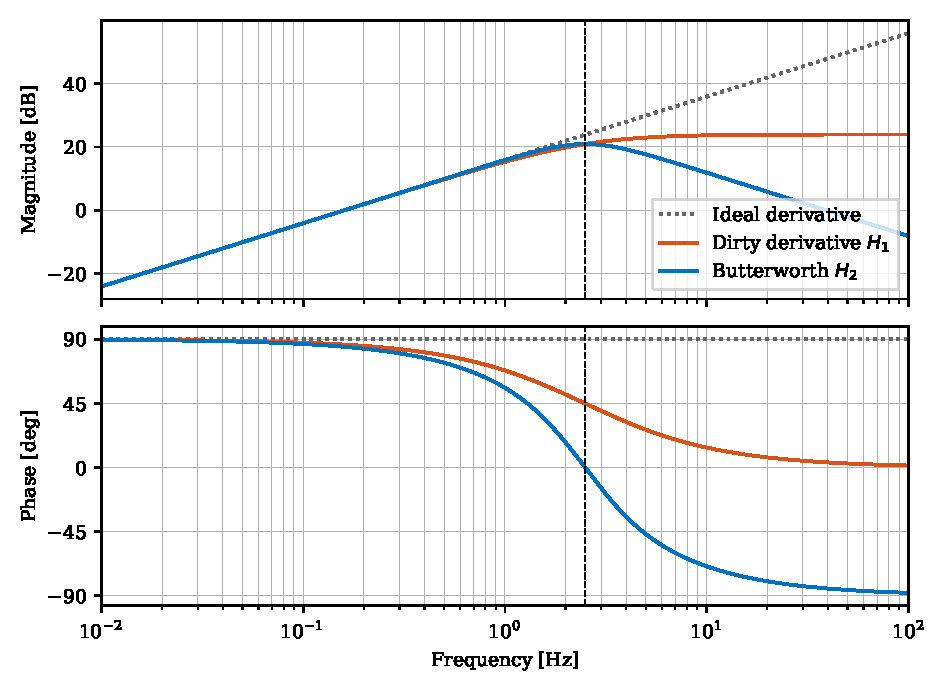
\includegraphics[width=0.85\textwidth]{figures/ch5/jerk_filters_bode.pdf}
    \caption{Bode diagrams of the dirty derivative $H_1$ and of the Butterworth filter $H_2$.}
    \label{fig:qff_bode}
\end{figure}

The activation thresholds of the flag are chosen by considering the jerk estimated from the
ground truth, by looking at its values when the vehicle is on a straight, i.e.\ with a slowly
varying dynamics, and when its dynamics changes, at the beginning and at the end of the
maneuvers, so that the latter exceed the upper threshold while the former remain mostly below
the lower one.

Once the jerk is estimated, the maneuver is detected through a hysteresis logic on its
magnitude, based on two thresholds $j_{\mathrm{on}} > j_{\mathrm{off}}$ and described by the
finite state machine of Fig.~\ref{fig:qff_fsm}. The flag is activated when the magnitude of the
jerk exceeds the upper threshold, and it is deactivated only when it falls below the lower
one. Between the two thresholds, the flag keeps its previous state, so that small oscillations
of the jerk around a single threshold do not switch it repeatedly, which limits the false
detections and the chattering of the flag.

\begin{figure}[H]
    \centering
    % Finite state machine of the maneuver flag (Chapter 5, feed-forward process noise).
\begin{tikzpicture}[
    font=\footnotesize,
    >={Stealth[length=2mm]},
    state/.style={circle, draw, thick, minimum size=21mm, align=center, font=\footnotesize},
    tr/.style={->, thick},
    lab/.style={font=\scriptsize, align=center, fill=white, inner sep=1.5pt}
]
\node[state, fill=black!5] (OFF) at (0,0) {\textbf{OFF}\\[2pt] $\mathbf{Q}_k = \mathbf{Q}_{\mathrm{nom}}$};
\node[state, fill=black!15] (ON) at (6,0) {\textbf{ON}\\[2pt] $\mathbf{Q}_k = \lambda\,\mathbf{Q}_{\mathrm{nom}}$};

% initial state
\coordinate (S) at (-2.6,0);
\fill (S) circle (2pt);
\draw[tr] (S) -- (OFF);

% transitions
\draw[tr] (OFF) to[bend left=22] node[lab, above]{$|j_k| > j_{\mathrm{on}}$} (ON);
\draw[tr] (ON) to[bend left=22] node[lab, below]{$|j_k| < j_{\mathrm{off}}$} (OFF);

% self loops
\draw[tr] (OFF) to[out=120, in=60, looseness=5] node[lab, above]{$|j_k| \le j_{\mathrm{on}}$} (OFF);
\draw[tr] (ON) to[out=120, in=60, looseness=5] node[lab, above]{$|j_k| \ge j_{\mathrm{off}}$} (ON);
\end{tikzpicture}

    \caption{Finite state machine of the maneuver flag.}
    \label{fig:qff_fsm}
\end{figure}

\subsection{Implementation}
\label{subsec:qff_implementation}
\label{sec:qff_implementation}

The main aspect of the implementation is the choice of the acceleration from which the jerk is
estimated. Deriving it from the filter whose process noise is switched would not allow the
maneuver to be detected in time. As shown in Fig.~\ref{fig:qff_highq}, with the nominal process
noise the acceleration follows the transitions with a delay, so that its derivative would
exceed the activation threshold only when the maneuver is already in progress, i.e.\ after the
delay that the method aims to reduce has been accumulated. The best estimate of the jerk is
instead obtained by differentiating the acceleration of the filter with the increased process
noise, which in Fig.~\ref{fig:qff_highq} is the closest to the ground truth at the changes of
maneuver, being the filter in its most reactive condition. Its larger noise is acceptable,
since this estimate is used only for the detection.

For this reason, the feed-forward approach is implemented with two filters that evolve in
parallel for each track and process the same measurements, according to the architecture of
Fig.~\ref{fig:qff_scheme}. The first is the main filter of Chapter~\ref{ch:tracking}, whose
process noise is switched by the hysteresis logic and whose state is published to the planning
module. The second, auxiliary, filter has the same structure, i.e.\ the EKF with the CCA model,
but its process noise is constant and increased, and it is used only to estimate the jerk and,
therefore, to drive the maneuver flag.

The auxiliary filter also avoids a coupling between the flag and the estimate. If the jerk were
derived from the main filter, the activation of the flag would inflate the process noise of
the same filter, making its acceleration noisier and its jerk larger, which would in turn keep
the flag active. The detection would then depend on its own output, in a feedback loop. Since
the process noise of the auxiliary filter does not depend on the flag, the detection is
decoupled from the switching, and the process noise of the main filter is set in feed-forward.

\begin{figure}[H]
    \centering
    % Architecture of the feed-forward process noise (Chapter 5).
\begin{tikzpicture}[
    font=\footnotesize,
    >={Stealth[length=2mm]},
    blk/.style={draw, thick, rounded corners=2pt, minimum width=22mm, minimum height=10mm, align=center},
    aux/.style={blk, fill=black!5},
    main/.style={blk, fill=black!15},
    arr/.style={->, thick},
    lab/.style={font=\scriptsize, align=center, fill=white, inner sep=1.2pt}
]
\node (Z) at (0,-1.4) {$\mathbf{z}_k$};
\coordinate (S) at (1.2,-1.4);
\node[aux]  (A) at (3.2,0)    {Auxiliary EKF\\ inflated $\mathbf{Q}$};
\node[aux]  (J) at (6.6,0)    {Jerk\\ estimation};
\node[aux]  (H) at (10,0)     {Hysteresis\\ logic};
\node[blk]  (Q) at (10,-2.8)  {Process noise\\ switch};
\node[main] (M) at (3.2,-2.8) {Main EKF\\ $\mathbf{Q}_k$};
\node (P) at (3.2,-4.6) {state published to the planning module};
\draw[thick] (Z) -- (S);
\draw[arr] (S) |- (A.west);
\draw[arr] (S) |- (M.west);
\draw[arr] (A) -- node[lab,above]{$a_k$} (J);
\draw[arr] (J) -- node[lab,above]{$j_k$} (H);
\draw[arr] (H) -- node[lab,right]{$f_k$} (Q);
\draw[arr] (Q) -- node[lab,above]{$\mathbf{Q}_{\mathrm{nom}}$ or $\lambda\mathbf{Q}_{\mathrm{nom}}$} (M);
\draw[arr] (M) -- (P);
\fill (S) circle (1.5pt);
\end{tikzpicture}

    \caption{Architecture of the feed-forward process noise.}
    \label{fig:qff_scheme}
\end{figure}

The jerk is estimated only on the updates that include the range rate of the RaDAR. Without it,
the acceleration of the auxiliary filter is corrected only through the position measurements,
which are separated from the jerk by three successive differentiations, so that the
corrections of the position would be strongly amplified in the jerk and would lead to false
activations of the flag. The jerk is estimated with the second-order Butterworth
filter~\eqref{eq:qff_butter}, the thresholds of the hysteresis are set to
$j_{\mathrm{on}} = \SI{15}{m/s^3}$ and $j_{\mathrm{off}} = \SI{5}{m/s^3}$, and the inflation
factor to $\lambda = 100$. Since the nominal spectral density of the acceleration is
$q_a = 5$, during the maneuvers the main filter adopts the same process noise as the auxiliary
one, i.e.\ the increased process noise of Fig.~\ref{fig:qff_highq}. The complete procedure is
reported in Algorithm~\ref{alg:qff}.

\begin{algorithm}[H]
\caption{Feed-forward process noise, for a single track.}
\label{alg:qff}
\begin{algorithmic}[1]
\REQUIRE nominal process noise $\mathbf{Q}_{\mathrm{nom}}$, inflation factor $\lambda$,
thresholds $j_{\mathrm{on}}$ and $j_{\mathrm{off}}$, previous flag $f_{k-1}$
\FORALL{measurements $\mathbf{z}_k$ associated with the track}
    \STATE update the auxiliary filter with $\mathbf{z}_k$ \COMMENT{increased process noise}
    \IF{$\mathbf{z}_k$ includes the range rate of the RaDAR}
        \STATE $a_k \leftarrow$ acceleration of the auxiliary filter
        \STATE $j_k \leftarrow$ filtered derivative of $a_k$ \COMMENT{\eqref{eq:qff_butter}}
        \IF{$|j_k| > j_{\mathrm{on}}$}
            \STATE $f_k \leftarrow 1$
        \ELSIF{$|j_k| < j_{\mathrm{off}}$}
            \STATE $f_k \leftarrow 0$
        \ELSE
            \STATE $f_k \leftarrow f_{k-1}$ \COMMENT{hysteresis, Fig.~\ref{fig:qff_fsm}}
        \ENDIF
    \ELSE
        \STATE $f_k \leftarrow f_{k-1}$
    \ENDIF
    \STATE $\mathbf{Q}_k \leftarrow \lambda\,\mathbf{Q}_{\mathrm{nom}}$ \textbf{if} $f_k = 1$ \textbf{else} $\mathbf{Q}_{\mathrm{nom}}$ \COMMENT{\eqref{eq:qff_switch}}
    \STATE predict the main filter with $\mathbf{Q}_k$ \COMMENT{\eqref{eq:qff_pred_cov}}
    \STATE correct the main filter with $\mathbf{z}_k$ \COMMENT{\eqref{eq:qff_gain}}
\ENDFOR
\end{algorithmic}
\end{algorithm}

% =====================================================================
\section{Results}
\label{sec:qff_results}

The feed-forward approach is evaluated on the session recorded on 5 September 2026 at Imola, by comparing the estimate of
the main filter with the feed-forward process noise against the one of the nominal filter and
the one of the filter with the increased process noise of Fig.~\ref{fig:qff_highq}, which
represent the two behaviors between which the method switches.

\begin{figure}[H]
    \centering
    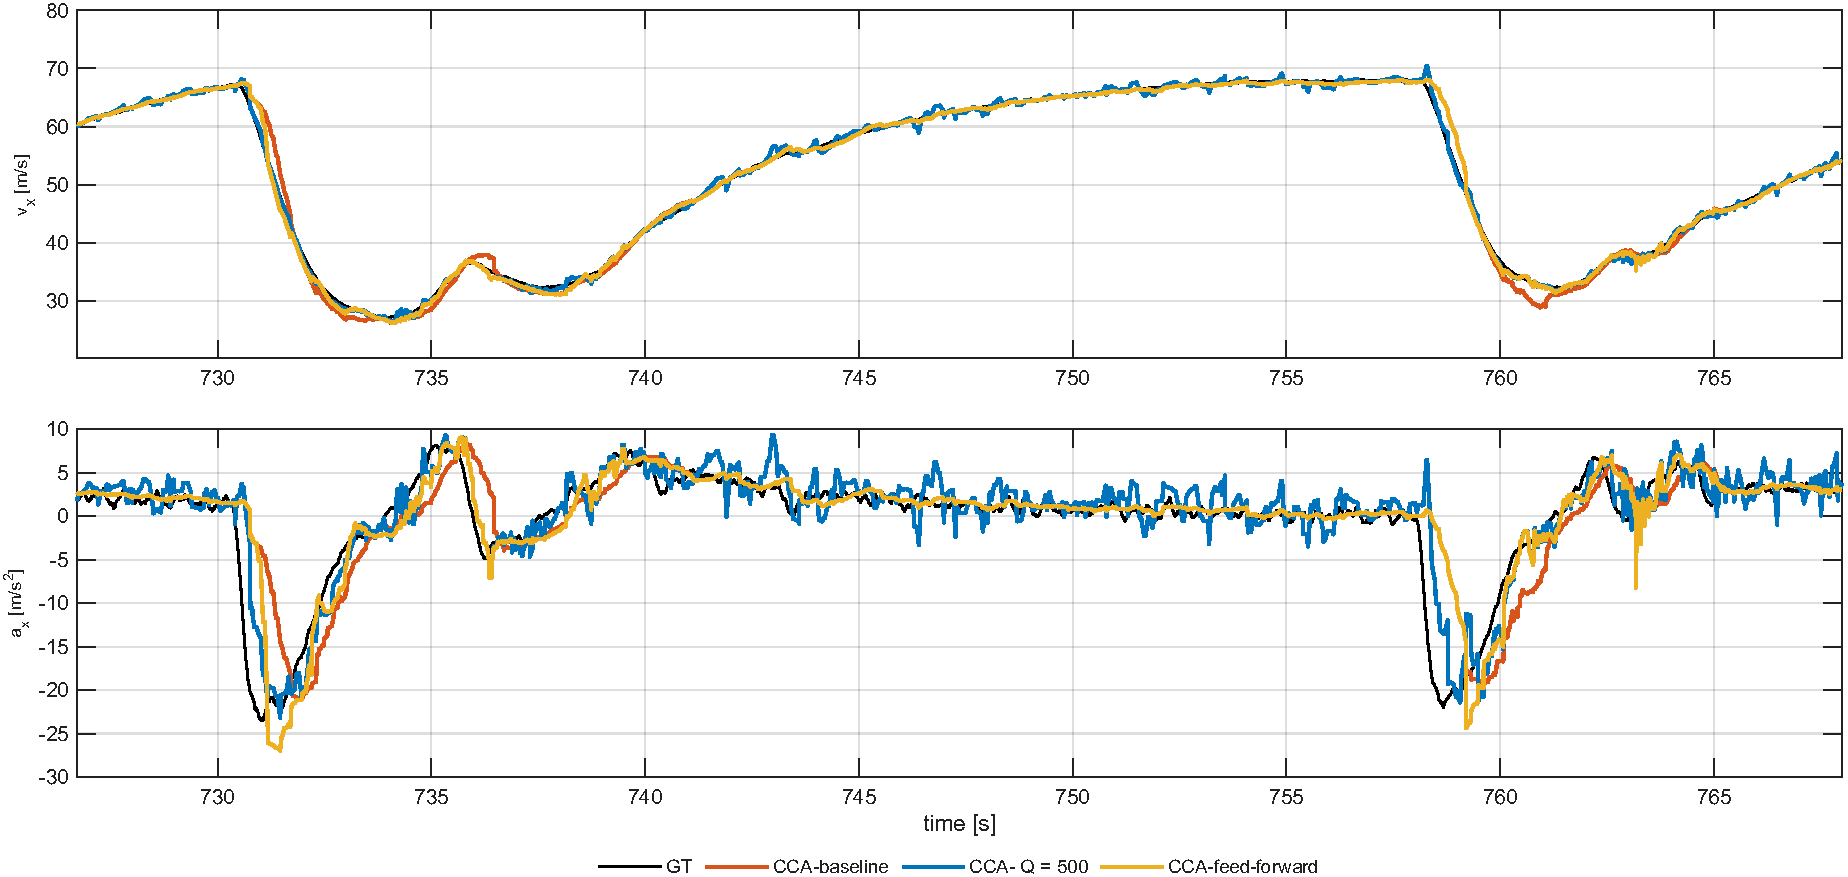
\includegraphics[width=\textwidth]{figures/ch5/qff_overview.pdf}
    \caption{Speed and acceleration estimated with the feed-forward process noise over a
    sequence of corners. Session of 5 September 2026, Imola.}
    \label{fig:qff_overview}
\end{figure}

Fig.~\ref{fig:qff_overview} shows the speed and the acceleration of the opponent over a
sequence that alternates braking phases with phases at almost constant speed. In the latter,
the estimate with the feed-forward process noise overlaps the nominal one and preserves its
smoothness, while the filter with the increased process noise follows the noise of the
measurements, which confirms that the flag remains inactive where the CCA model is adequate.
In the two braking phases between \SI{730}{s} and \SI{740}{s}, the flag is activated and the
feed-forward estimate approximates the ground truth better than the nominal filter, following
the drop of the acceleration earlier and with a smaller delay on the speed. The braking at
about \SI{760}{s}, instead, clearly shows the limit of the method. The flag is activated late,
when the deceleration is already in progress, so that during the braking the feed-forward
estimate accumulates the same delay as the nominal one, and it departs from it only in the
following phase of traction.

\begin{figure}[H]
    \centering
    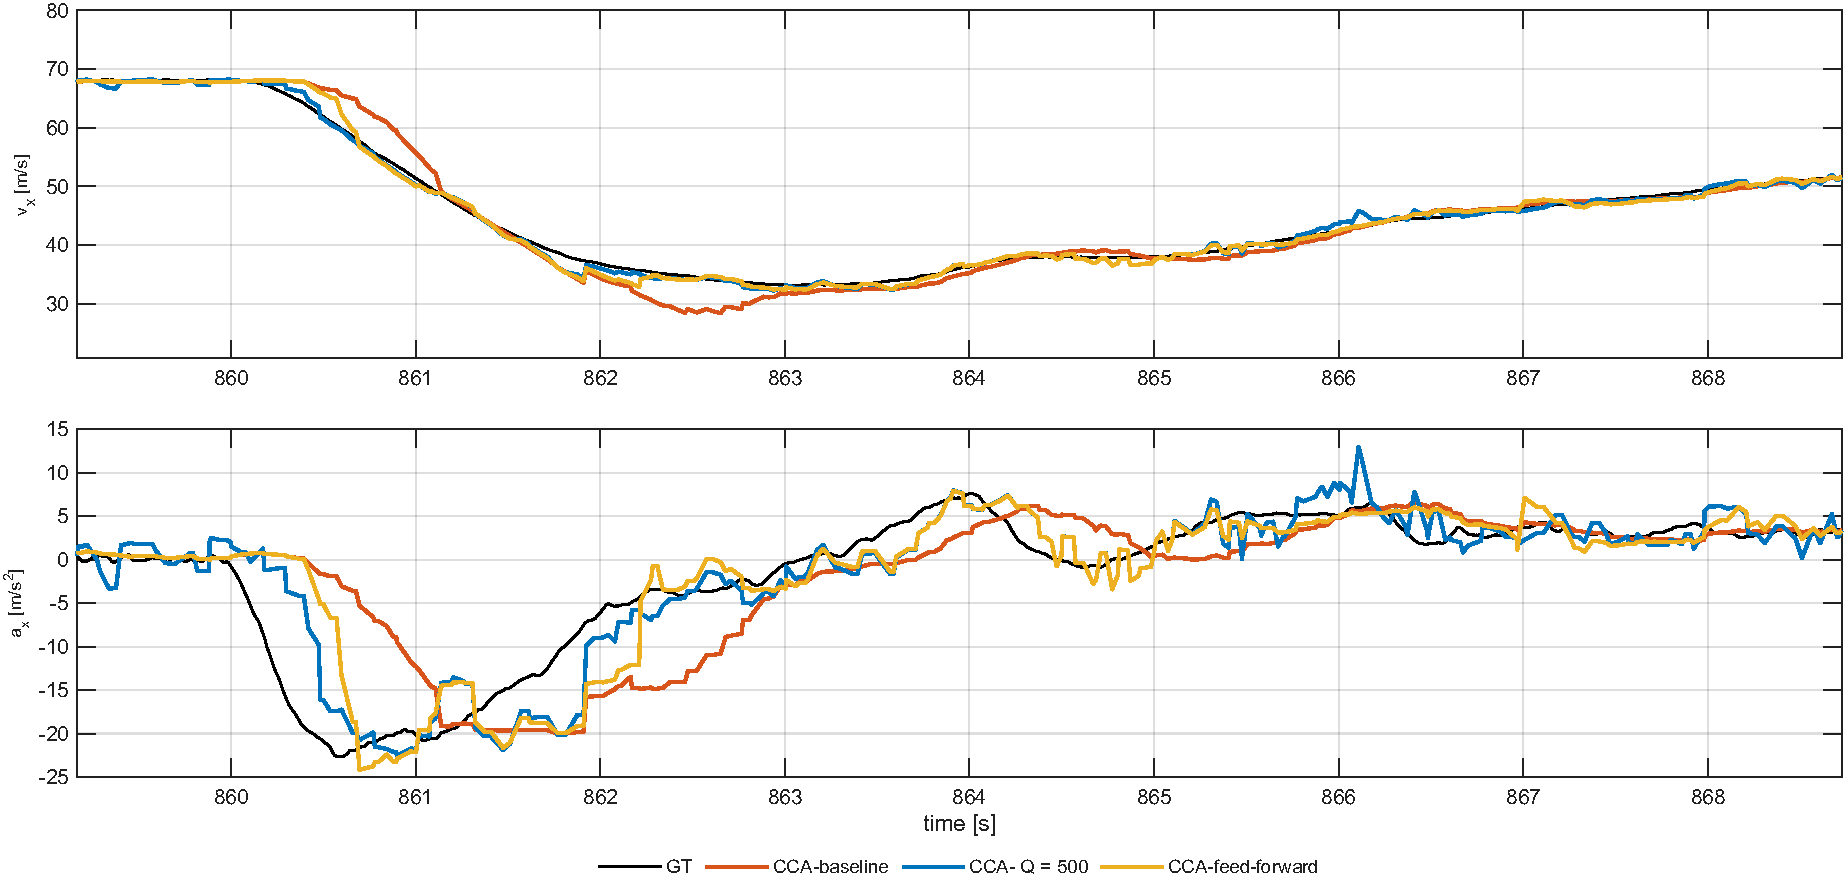
\includegraphics[width=\textwidth]{figures/ch5/qff_braking_detail.pdf}
    \caption{Detail of a braking phase. Session of 5 September 2026, Imola.}
    \label{fig:qff_braking_detail}
\end{figure}

The detail of Fig.~\ref{fig:qff_braking_detail} shows a braking in which the maneuver is
correctly detected. The feed-forward estimate starts to decrease with a slight delay with
respect to the filter with the increased process noise, but well before the nominal one,
whose delay is accumulated in the speed, which is underestimated at the end of the braking. The
feed-forward process noise therefore evidently improves the estimate of the nominal model, and
its speed remains close to the ground truth during the whole maneuver.

\begin{figure}[H]
    \centering
    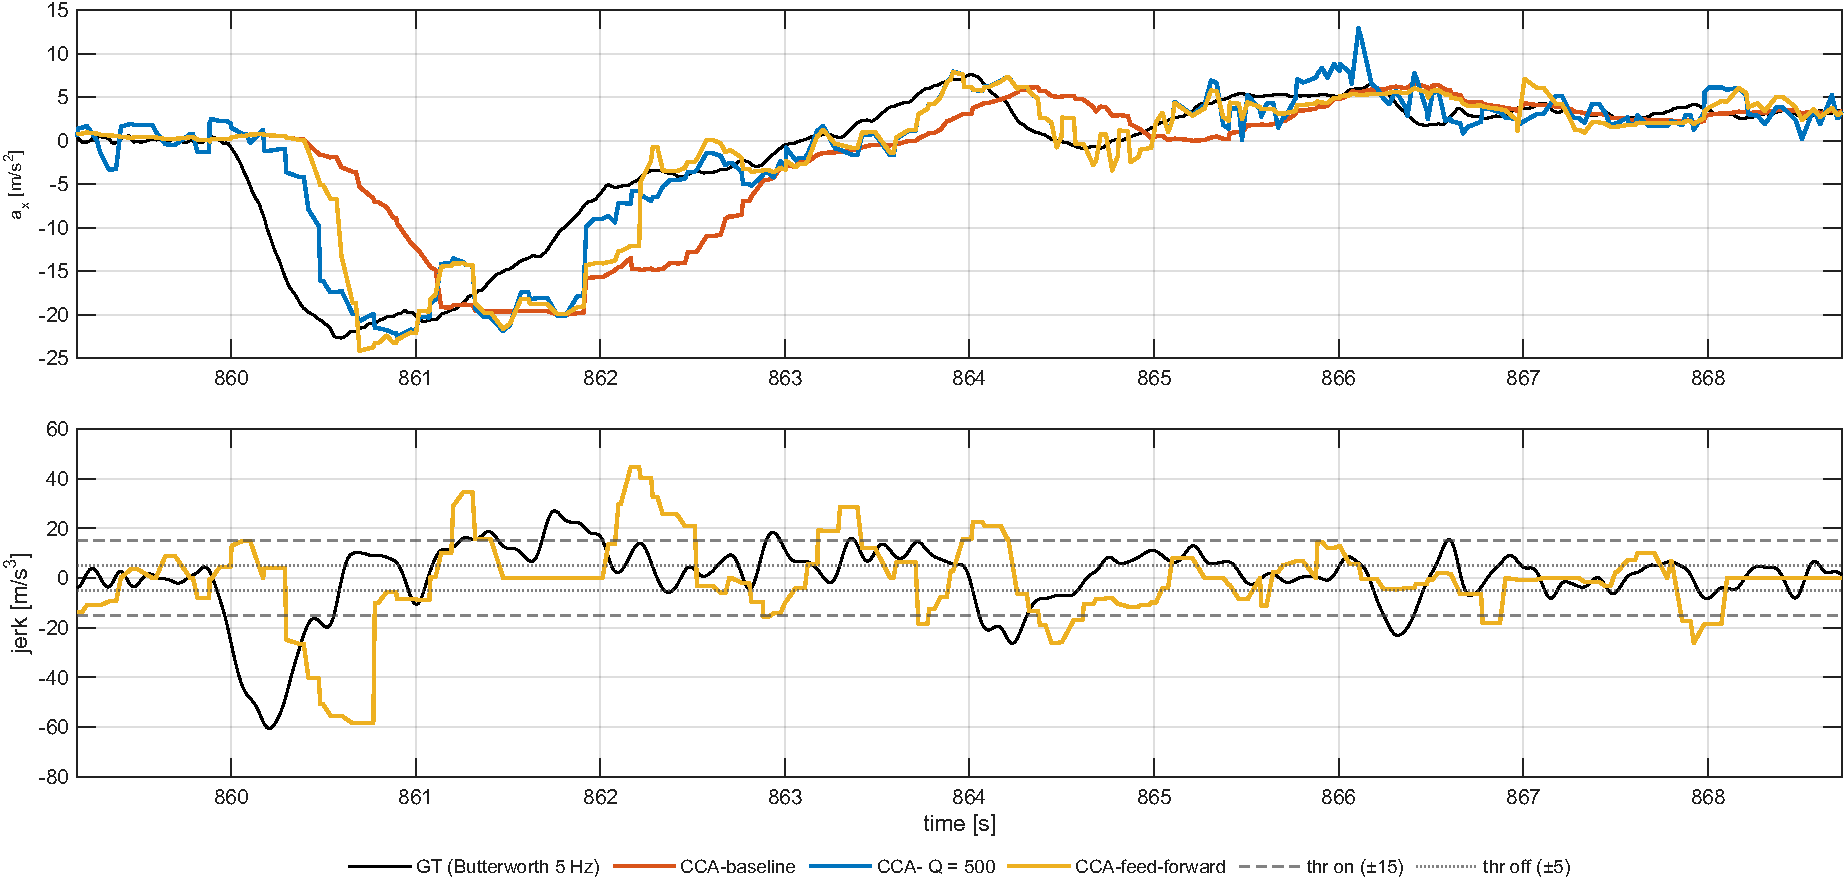
\includegraphics[width=\textwidth]{figures/ch5/qff_jerk.pdf}
    \caption{Acceleration and estimated jerk, with the activation thresholds of the flag, for
    the braking of Fig.~\ref{fig:qff_braking_detail}. Session of 5 September 2026, Imola.}
    \label{fig:qff_jerk}
\end{figure}

Fig.~\ref{fig:qff_jerk} complements Fig.~\ref{fig:qff_braking_detail} with the jerk estimated
from the auxiliary filter, compared with the jerk of the ground truth and with the thresholds
of the hysteresis. The estimated jerk detects the onset of the braking, but its main peak
follows the one of the ground truth with a slight delay, which is directly reflected on the
activation of the flag and explains the delay of the feed-forward estimate with respect to the
filter with the increased process noise. Moreover, in some intervals after the braking, the
estimated jerk exceeds the upper threshold while the jerk of the ground truth remains small,
causing spurious activations of the flag.

\begin{figure}[H]
    \centering
    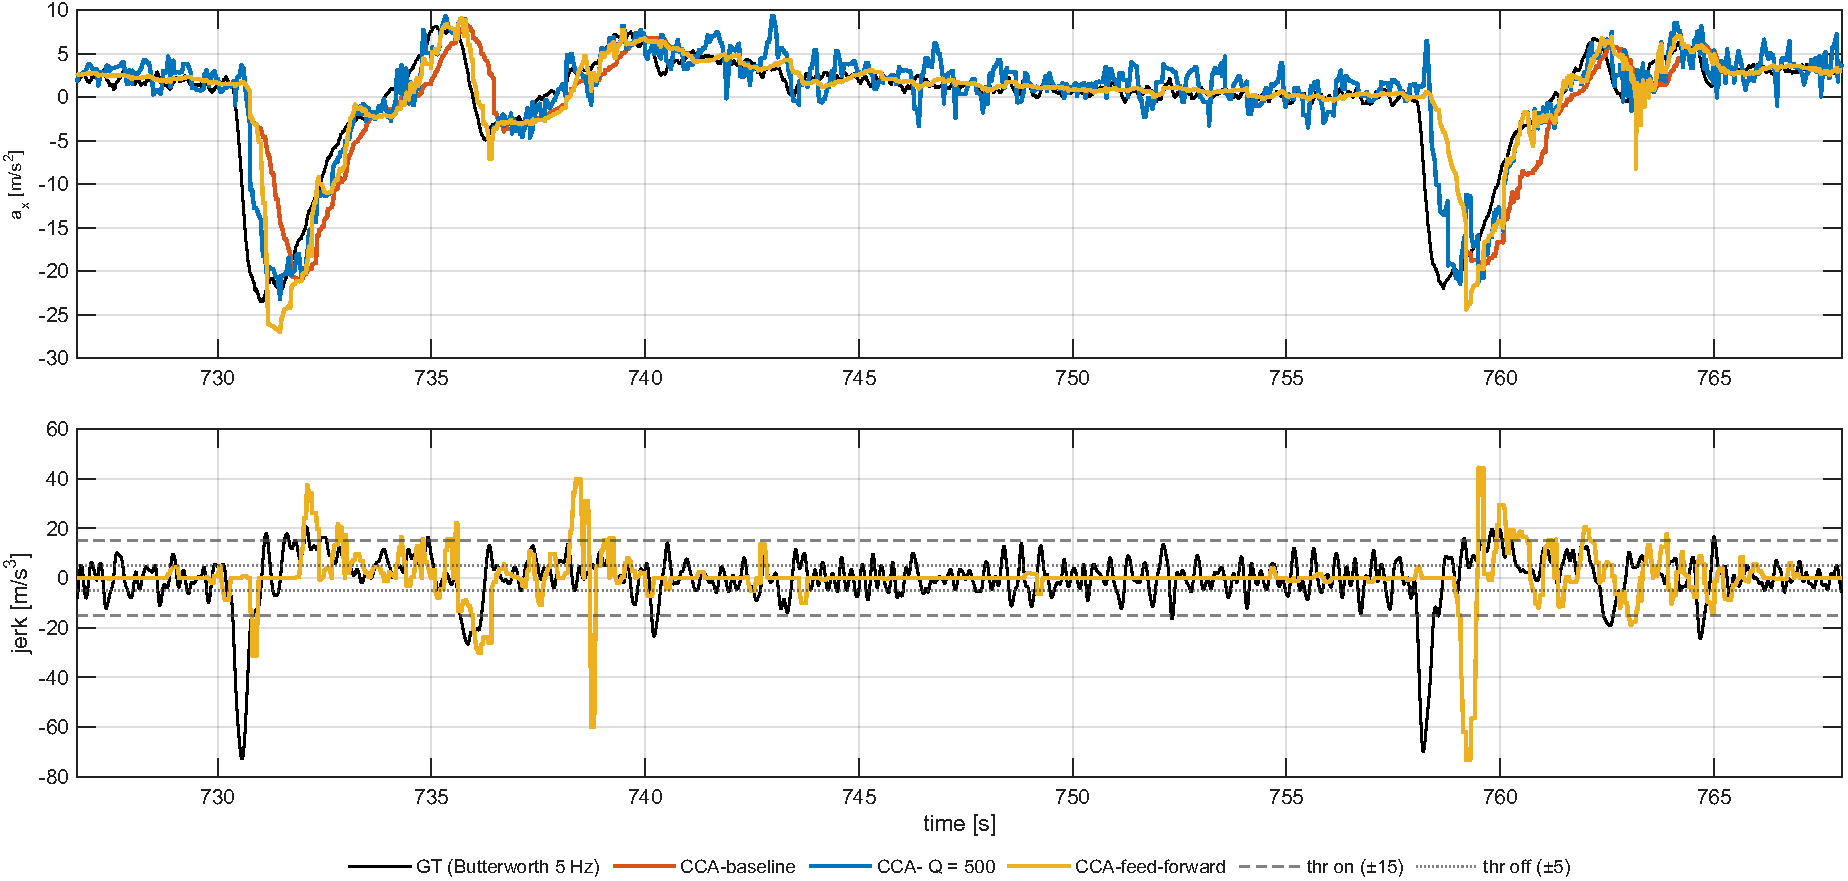
\includegraphics[width=\textwidth]{figures/ch5/qff_jerk_overview.pdf}
    \caption{Acceleration and estimated jerk, with the activation thresholds of the flag, for
    the maneuvers of Fig.~\ref{fig:qff_overview}. Session of 5 September 2026, Imola.}
    \label{fig:qff_jerk_overview}
\end{figure}

The same considerations hold for Fig.~\ref{fig:qff_jerk_overview}, which shows the jerk for
the maneuvers of Fig.~\ref{fig:qff_overview}. In particular, it shows the reason for the late
activation at about \SI{760}{s}. The jerk of the ground truth exhibits a sharp peak at the
onset of the braking, but the estimated jerk only reaches the upper threshold about one second
later, when the braking is already well developed, so that the delay of the feed-forward
estimate is entirely due to the delay of the estimator. Also in this case, isolated peaks of
the estimated jerk, e.g.\ at about \SI{739}{s}, exceed the thresholds while the jerk of the
ground truth remains small, leading to spurious activations.

Overall, the approach works and its principle is correct, since the flag remains inactive in
the phases at constant acceleration and is activated in the braking and traction phases, so
that the filter with the feed-forward process noise lies between the nominal filter and the one
with the increased process noise, keeping the smoothness of the former where the dynamics
changes slowly and approaching the reactivity of the latter during the maneuvers. The method,
however, presents limits related to the quality of the jerk estimator. Since the jerk is
ultimately obtained by differentiating the acceleration of the filter with the increased
process noise, it inherits the delay with which this filter follows the changes of the
dynamics, which is transferred to the activation of the flag, and the differentiation amplifies
part of its noise, which produces spurious activations also in phases in which the dynamics of
the opponent is not excited. In this perspective, the flag and its thresholds represent the
tuning knob of the method, since raising the activation threshold $j_{\mathrm{on}}$ reduces the
spurious activations but, at the same time, introduces a further delay in the activation when
an actual maneuver occurs.

\chapter{RTS Smoother}
\label{ch:rts}

The tracker described in Chapter~\ref{ch:tracking} is a causal filter, i.e.\ the estimate
at each instant is computed only from the measurements received up to that instant. This
limits the quality of the estimate during the maneuvers. The CCA model assumes a constant
acceleration over each prediction interval, while on track the opponent alternates
braking, cornering and traction phases, in which the acceleration changes abruptly. In
these phases the filter can only follow the new dynamics after the measurements have shown
it, and the estimate lags behind the true state of the opponent.

An alternative approach to improve the quality of the estimate of the state of the
opponent during the maneuvers is presented in this chapter, and consists in the
implementation of an acausal filter. The idea is to exploit the future information, i.e.\
the measurements acquired after each instant, to refine the estimate of the past states of
the opponent. This is the purpose of a smoother, an acausal estimator that computes the
state at each instant from the measurements acquired both before and after it.

This choice is also made possible by the fact that, in the application, the estimate of
the opponent is used by the planning module to perform the gap control, i.e.\ to regulate
the distance from the opponent in terms of time. For this purpose, the real-time estimate
of the state of the opponent is not strictly necessary, and a past estimate can also be
used, provided that it is more accurate.

Specifically, among the smoothing algorithms, the Rauch--Tung--Striebel (RTS) smoother is
adopted. It comes in handy since it reuses the causal estimate of the Kalman filter and
enhances it with a backward recursion, so that it can be added to the existing tracker
without modifying it.

Section~\ref{sec:rts_problem} introduces the smoothing problem and its relation with
filtering and prediction. Section~\ref{sec:rts_formulation} derives the RTS smoother and its application on a
sliding window of the history.
Section~\ref{sec:rts_implementation} describes its implementation in the target tracking
module. Finally, Section~\ref{sec:rts_sensitivity} analyzes the effect of the window
length on the smoothed estimate, with and without the RaDAR measurements.

% =====================================================================
\section{From Filtering to Smoothing}
\label{sec:rts_problem}

Given the set of measurements $\mathbf{Y}_N = \{\mathbf{z}_1, \dots, \mathbf{z}_N\}$, the
estimate of the state $\mathbf{x}_k$ at instant $k$ is the value that maximizes the
conditional probability density of the state given the measurements,
\begin{equation}
    \hat{\mathbf{x}}_{k|N} = \arg\max_{\mathbf{x}_k}\; p\left(\mathbf{x}_k \mid \mathbf{Y}_N\right).
    \label{eq:rts_map}
\end{equation}
Depending on the relation between $k$ and the last measurement $N$, three problems are
distinguished.
\begin{itemize}
    \item \textbf{Prediction}, with $N < k$, in which the measurements stop before the
    instant of interest and the state is extrapolated through the model.
    \item \textbf{Filtering}, with $N = k$, in which the measurements are available up to
    the instant of interest. This is the problem solved by the Kalman filter.
    \item \textbf{Smoothing}, with $N > k$, in which also the measurements acquired after
    the instant of interest are used.
\end{itemize}
The three problems share the same conditional density, and only the information used to
compute it changes. The Kalman filter, introduced in 1960, solves the filtering problem.
In 1965, Rauch, Tung and Striebel showed that the smoothing problem can be solved from
the same principle, i.e.\ the maximization of the likelihood, and in a recursive form,
which runs backward on the output of the Kalman filter.

An alternative solution is given by the two-filter approach of Fraser and Potter, in
which the smoothed estimate is obtained as the combination of two Kalman filters, one
running forward from the first measurement and one running backward from the last one.
The two formulations have been proven to be equivalent. In this work, the RTS formulation is chosen since it is more convenient
from an implementation point of view. It exploits the quantities already computed by the
forward filter, which only have to be stored, and it is lighter, since it does not require
a second filter running in parallel, with its own initialization. The backward recursion
is instead initialized with the estimate of the forward filter at the current time.

% =====================================================================
\section{RTS Smoother Formulation}
\label{sec:rts_formulation}

The derivation is first presented for a linear system,
\begin{equation}
    \mathbf{x}_{k+1} = \mathbf{F}_k\,\mathbf{x}_k + \mathbf{w}_k,
    \qquad
    \mathbf{z}_k = \mathbf{H}_k\,\mathbf{x}_k + \mathbf{v}_k,
    \label{eq:rts_linear}
\end{equation}
with $\mathbf{w}_k$ and $\mathbf{v}_k$ zero-mean Gaussian white noises with covariance
$\mathbf{Q}_k$ and $\mathbf{R}_k$. For the EKF of the tracker, $\mathbf{F}_k$ is the
Jacobian~\eqref{eq:tt_F} of the motion model, evaluated at the filtered estimate.

\subsection{Forward Pass}
\label{subsec:rts_forward}

The forward pass is the Kalman filter of Chapter~\ref{ch:tracking}. At each step, the
state is predicted,
\begin{equation}
    \hat{\mathbf{x}}_{k+1|k} = \mathbf{F}_k\,\hat{\mathbf{x}}_{k|k},
    \qquad
    \mathbf{P}_{k+1|k} = \mathbf{F}_k\,\mathbf{P}_{k|k}\,\mathbf{F}_k^\top + \mathbf{Q}_k,
    \label{eq:rts_fwd_pred}
\end{equation}
and then corrected with the measurement,
\begin{equation}
    \begin{aligned}
        \mathbf{K}_{k+1} &= \mathbf{P}_{k+1|k}\,\mathbf{H}_{k+1}^\top
        \left(\mathbf{H}_{k+1}\,\mathbf{P}_{k+1|k}\,\mathbf{H}_{k+1}^\top + \mathbf{R}_{k+1}\right)^{-1}, \\
        \hat{\mathbf{x}}_{k+1|k+1} &= \hat{\mathbf{x}}_{k+1|k}
        + \mathbf{K}_{k+1}\left(\mathbf{z}_{k+1} - \mathbf{H}_{k+1}\,\hat{\mathbf{x}}_{k+1|k}\right),
    \end{aligned}
    \label{eq:rts_fwd_corr}
\end{equation}
as in~\eqref{eq:tt_prediction} and~\eqref{eq:tt_update}. For the backward step, the
prior estimate $\hat{\mathbf{x}}_{k+1|k}$ and its covariance $\mathbf{P}_{k+1|k}$ are
stored at every step, together with the state matrix $\mathbf{F}_k$, to compute the
smoothed estimate.

\subsection{Backward Recursion}
\label{subsec:rts_backward}

The backward recursion is derived from the joint probability density of two consecutive
states and of the measurements, $p(\mathbf{x}_k, \mathbf{x}_{k+1}, \mathbf{Y}_N)$.
Applying the Markov property of the model, i.e.\ once $\mathbf{x}_{k+1}$ is given the
future measurements $\mathbf{z}_{k+1}, \dots, \mathbf{z}_N$ do not depend on
$\mathbf{x}_k$, the density can be factorized as
\begin{equation}
    p(\mathbf{x}_k, \mathbf{x}_{k+1}, \mathbf{Y}_N) =
    p(\mathbf{z}_{k+1}, \dots, \mathbf{z}_N \mid \mathbf{x}_{k+1})\;
    p(\mathbf{x}_{k+1} \mid \mathbf{x}_k)\;
    p(\mathbf{x}_k \mid \mathbf{Y}_k)\;
    p(\mathbf{Y}_k),
    \label{eq:rts_joint}
\end{equation}
This factorization links the step $k$ to the step $k+1$, whose smoothed estimate is
already available from the previous backward step, and is the origin of the recursion.
In~\eqref{eq:rts_joint}, only the second and the third terms depend on $\mathbf{x}_k$.
Both are Gaussian, the first with mean $\mathbf{F}_k\,\mathbf{x}_k$ and covariance
$\mathbf{Q}_k$, the second with mean $\hat{\mathbf{x}}_{k|k}$ and covariance
$\mathbf{P}_{k|k}$, given by the forward pass. Taking the logarithm, the smoothed estimate
$\hat{\mathbf{x}}_{k|N}$ is the value that minimizes the cost function
\begin{equation}
    J(\mathbf{x}_k) =
    \left\|\hat{\mathbf{x}}_{k+1|N} - \mathbf{F}_k\,\mathbf{x}_k\right\|^2_{\mathbf{Q}_k^{-1}}
    + \left\|\mathbf{x}_k - \hat{\mathbf{x}}_{k|k}\right\|^2_{\mathbf{P}_{k|k}^{-1}},
    \label{eq:rts_cost}
\end{equation}
in which $\mathbf{x}_{k+1}$ has been replaced by its smoothed estimate. The cost function
contains two terms. The first measures the consistency with the future, i.e.\ the mismatch
between the smoothed state at $k+1$ and the prediction propagated from $\mathbf{x}_k$,
weighted by the inverse of the process noise covariance. The second measures the
consistency with the past, i.e.\ the distance from the filtered estimate, weighted by the
inverse of its covariance. Setting the gradient of $J$ to zero and applying the matrix
inversion lemma gives the smoother gain
\begin{equation}
    \mathbf{C}_k = \mathbf{P}_{k|k}\,\mathbf{F}_k^\top
    \left(\mathbf{F}_k\,\mathbf{P}_{k|k}\,\mathbf{F}_k^\top + \mathbf{Q}_k\right)^{-1}
    = \mathbf{P}_{k|k}\,\mathbf{F}_k^\top\,\mathbf{P}_{k+1|k}^{-1},
    \label{eq:rts_gain}
\end{equation}
the smoothed estimate
\begin{equation}
    \hat{\mathbf{x}}_{k|N} = \hat{\mathbf{x}}_{k|k}
    + \mathbf{C}_k\left(\hat{\mathbf{x}}_{k+1|N} - \hat{\mathbf{x}}_{k+1|k}\right),
    \label{eq:rts_state}
\end{equation}
and its covariance
\begin{equation}
    \mathbf{P}_{k|N} = \mathbf{P}_{k|k}
    + \mathbf{C}_k\left(\mathbf{P}_{k+1|N} - \mathbf{P}_{k+1|k}\right)\mathbf{C}_k^\top.
    \label{eq:rts_cov}
\end{equation}

The smoother gain has the same structure as the Kalman gain in~\eqref{eq:rts_fwd_corr},
with the substitution of $\mathbf{H}_{k+1}$ with $\mathbf{F}_k$, of $\mathbf{R}_{k+1}$ with
$\mathbf{Q}_k$ and of $\mathbf{P}_{k+1|k}$ with $\mathbf{P}_{k|k}$. In the Kalman filter,
the measurement corrects the predicted state. In the smoother, the smoothed state at
$k+1$ acts as a pseudo-measurement that corrects the filtered state at $k$.

The correction of the acausal state depends on two factors. The first is the mismatch
between the prediction $\hat{\mathbf{x}}_{k+1|k}$ and the smoothed state
$\hat{\mathbf{x}}_{k+1|N}$. If the model is correct, the mismatch is small and the
smoothed state remains close to the causal one. If instead the dynamics of the opponent
has changed, e.g.\ at the beginning of a maneuver, the smoothed state differs from the
prediction and the mismatch is larger. The mismatch is then weighted by the gain
$\mathbf{C}_k$, which incorporates the uncertainty of the filter through
$\mathbf{P}_{k|k}$. If the filter is not very uncertain, the gain is small and the
smoother corrects little, since the filtered estimate does not need the future
information. If the filter is uncertain, the gain is larger and the future information
weighs more on the smoothed estimate.

The recursion is initialized at the last step, $k = N$, where the measurements used by
the filter and by the smoother coincide, so that the filtered estimate
$\hat{\mathbf{x}}_{N|N}$ and its covariance $\mathbf{P}_{N|N}$ are also the smoothed
ones. The recursion~\eqref{eq:rts_gain}--\eqref{eq:rts_cov} is then applied backward, for
$k = N-1, \dots, 0$.

\subsection{Fixed-Lag Smoothing on a Sliding Window}
\label{subsec:rts_window}

The formulation above refers to a fixed interval, in which all the measurements are
available before the backward pass starts. In the tracker, the measurements keep
arriving, and the smoother is applied on a sliding window of duration $T_w$, which
contains the steps to be smoothed, between $t_N - T_w$ and the most recent one $t_N$. The
smoother acts on the history of the opponent that is passed to the planning module. At
every publication, the backward pass is run on the whole window, starting from the most
recent step. As the window slides, each past state is smoothed again with the newly
available measurements, and its estimate is progressively refined. The estimate of a
state at a time $d$ before the most recent step, here referred to as buffer age, is
obtained with $d$ seconds of future measurements, so that the buffer age plays the role of
the lag of a fixed-lag smoother. The complete algorithm is reported in
Algorithm~\ref{alg:rts}.

\begin{algorithm}[H]
\caption{RTS smoother on the sliding window of the history, for a single track.}
\label{alg:rts}
\begin{algorithmic}[1]
\REQUIRE entries $k = 0, \dots, N$ of the history of the track in the window
$[t_N - T_w,\, t_N]$, storing $\hat{\mathbf{x}}_{k|k}$, $\mathbf{P}_{k|k}$,
$\hat{\mathbf{x}}_{k+1|k}$, $\mathbf{P}_{k+1|k}$ and $\mathbf{F}_k$
\ENSURE smoothed estimates $\hat{\mathbf{x}}_{k|N}$ and $\mathbf{P}_{k|N}$
\IF{the smoother is disabled \OR $N < 1$}
    \RETURN the causal estimates
\ENDIF
\STATE $\hat{\mathbf{x}}_{N|N},\, \mathbf{P}_{N|N} \leftarrow$ filtered estimate \COMMENT{initialization}
\FOR{$k = N-1$ \textbf{down to} $0$}
    \IF{the prediction $\hat{\mathbf{x}}_{k+1|k}$, $\mathbf{P}_{k+1|k}$ is stored}
        \STATE $\mathbf{C}_k \leftarrow \mathbf{P}_{k|k}\,\mathbf{F}_k^\top\,\mathbf{P}_{k+1|k}^{-1}$
        \STATE $\hat{\mathbf{x}}_{k|N} \leftarrow \hat{\mathbf{x}}_{k|k} + \mathbf{C}_k\left(\hat{\mathbf{x}}_{k+1|N} - \hat{\mathbf{x}}_{k+1|k}\right)$
        \STATE $\mathbf{P}_{k|N} \leftarrow \mathbf{P}_{k|k} + \mathbf{C}_k\left(\mathbf{P}_{k+1|N} - \mathbf{P}_{k+1|k}\right)\mathbf{C}_k^\top$
    \ELSE
        \STATE $\hat{\mathbf{x}}_{k|N},\, \mathbf{P}_{k|N} \leftarrow$ filtered estimate \COMMENT{causal fallback}
    \ENDIF
\ENDFOR
\RETURN $\hat{\mathbf{x}}_{k|N}$, $\mathbf{P}_{k|N}$ for $k = 0, \dots, N$
\end{algorithmic}
\end{algorithm}

% =====================================================================
\section{Implementation}
\label{sec:rts_implementation}

The smoother is implemented as a read-only layer on top of the causal filter. It never
writes back into the EKF, so that the forward pass, the life cycle of the tracks and the
current state published to the planning module remain unchanged. The smoothed states are
stored alongside the causal ones, and the smoother can be disabled through a parameter,
which restores the original behavior of the tracker.

The smoother relies on the history of the tracker already introduced for the
out-of-sequence measurements (Section~\ref{subsec:tt_oosm}), in which each entry contains
the state of all the tracks after the processing of a measurement. In the prediction step
of the EKF, right after the propagation and before the correction, the predicted state
$\hat{\mathbf{x}}_{k+1|k}$, its covariance $\mathbf{P}_{k+1|k}$ and the Jacobian
$\mathbf{F}_k$ are stored in the track, so that each entry of the history contains all the
quantities required by the backward pass.

At every publication, the window $[t_N - T_w,\, t_N]$ is extracted from the history, with
$t_N$ the time of the most recent entry, and at least two entries are required to run the
smoother. The backward pass then pairs each entry $k$ with the following one $k+1$, and
for each track of entry $k$ looks for the same track in entry $k+1$. The future state is
the one smoothed at the previous iteration or, when it is not available, the causal one.
Only the state and the covariance are replaced by the smoothed ones, while the other
fields of the track, such as its identifier and timestamp, are copied from the causal
estimate. Every degenerate case, such as a track that has just been initialized or a state
without future support, falls back to the causal estimate, so that the output is always
complete.

The implementation is also robust to the out-of-sequence measurements. When a late
measurement arrives, the tracker inserts it in the history according to its acquisition
time and reprocesses all the following entries (Section~\ref{subsec:tt_oosm}), so that
the filtered states, the predictions and the Jacobians stored in the history are updated.
Since the smoother never modifies the history and recomputes the whole window from the
stored quantities at every publication, the late measurement is automatically included
in the next backward pass, and no smoothed state has to be corrected or invalidated.

The history published to the planning module contains, at the current time, the causal
prediction of the Kalman filter, without any correction. From the first available
measurement backward, it contains the smoothed history, using the smoothed state when it
is available and the causal one otherwise. In this way, the most recent state of the
opponent is published without any additional delay, and its past states benefit from the
future measurements.

% =====================================================================
\section{Sensitivity Analysis}
\label{sec:rts_sensitivity}

The main parameter of the smoother is the window length $T_w$, which sets how much future
information is available to smooth each state. In the following, the estimates are
compared at different window lengths, i.e.\ at different buffer ages, where a window of
\SI{0}{ms} corresponds to the most recent filtered estimate, i.e.\ the correction, and a
negative window to the causal prediction at the publication time. The effect of the
window is evaluated on the speed of the opponent, compared with the ground truth through
two metrics.
\begin{itemize}
    \item \textbf{RMSE of the speed}, computed between the estimate at a given window
    length and the ground truth at the corresponding time, both on the whole session
    (global RMSE) and on the braking phases only (local RMSE).
    \item \textbf{Maneuver delay}, i.e.\ the time difference between the instant at which the
    estimated speed starts a braking maneuver and the same instant for the ground truth. A
    positive value indicates that the estimate starts the maneuver late, a negative one
    that it anticipates it. The braking maneuvers are identified on the ground truth, 63
    in the session analyzed, and the delay is summarized by its median over the
    maneuvers for which the start of the braking is detected in the estimate, i.e.\ 49
    with all the sensors and 44 without the RaDAR.
\end{itemize}

The window length is analyzed on the session recorded on the day of the race at Imola, on
5 September 2026. The sensitivity analysis is carried out first with the measurements of
all the sensors, and then removing the measurements of the RaDAR, i.e.\ the measurement of
the speed. With all the sensors, Fig.~\ref{fig:rts_lag_radar} shows the speed of the
opponent during a braking phase and a full corner. The prediction is the causal estimate
of the filter at the publication time, the correction is the most recent filtered
estimate, and the other curves are the smoothed estimates obtained with windows from 100
to \SI{500}{ms}. As the window increases, the smoothed estimate moves closer to the
ground truth, both at the beginning of the braking and around the apex of the corner. With
the RaDAR, the curves obtained with windows longer than about \SI{200}{ms} are almost
superimposed.

\begin{figure}[!htbp]
    \centering
    \subfloat[Braking]{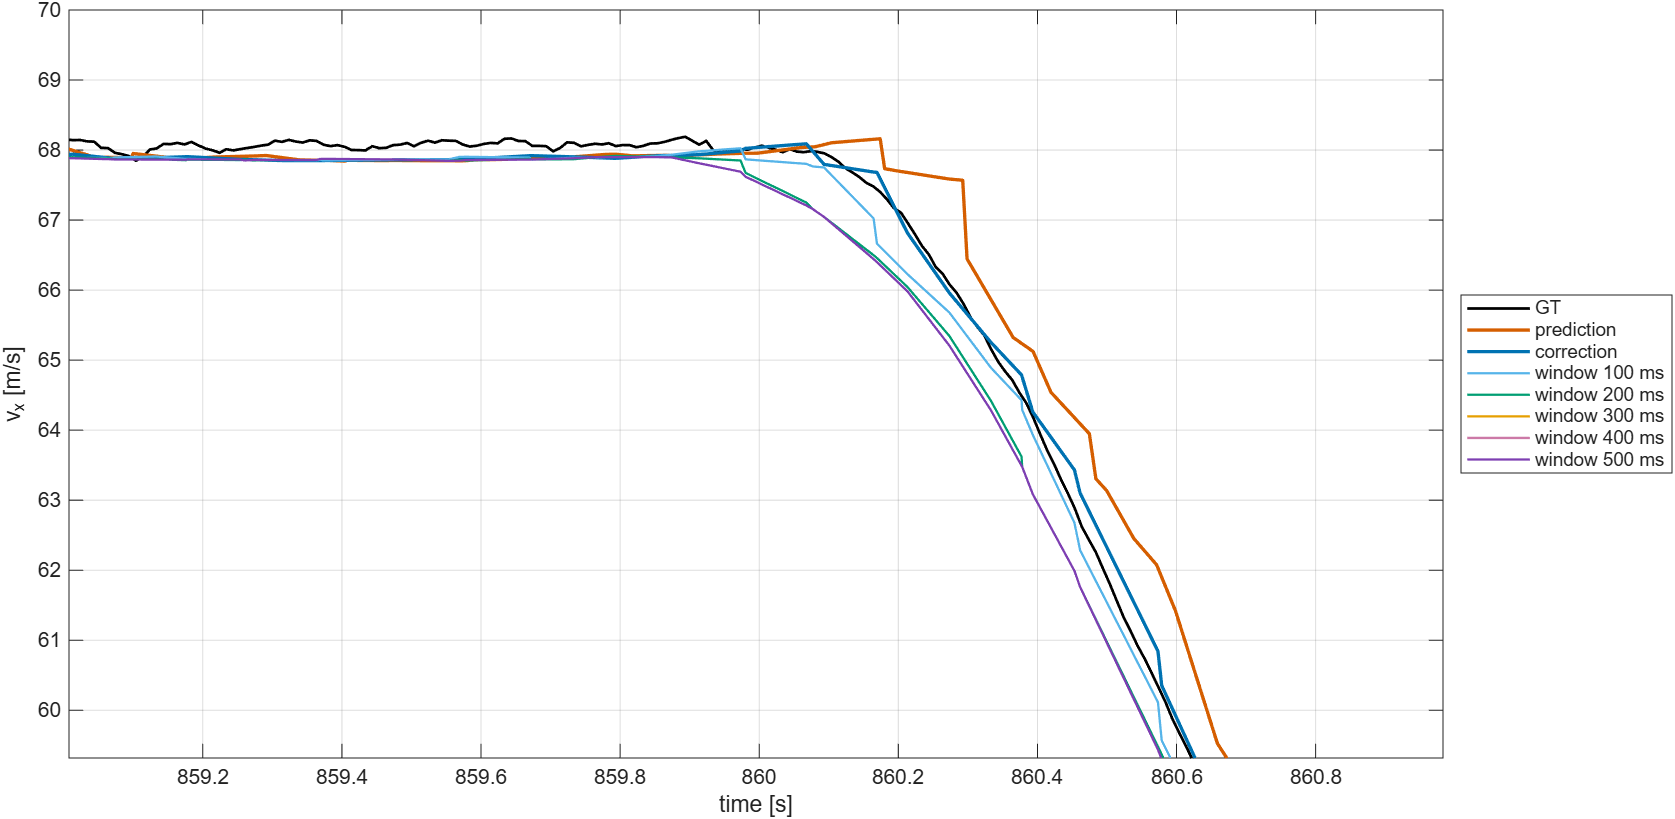
\includegraphics[width=0.76\textwidth]{figures/ch6/rts_lag_radar_braking.png}}\\
    \subfloat[Corner]{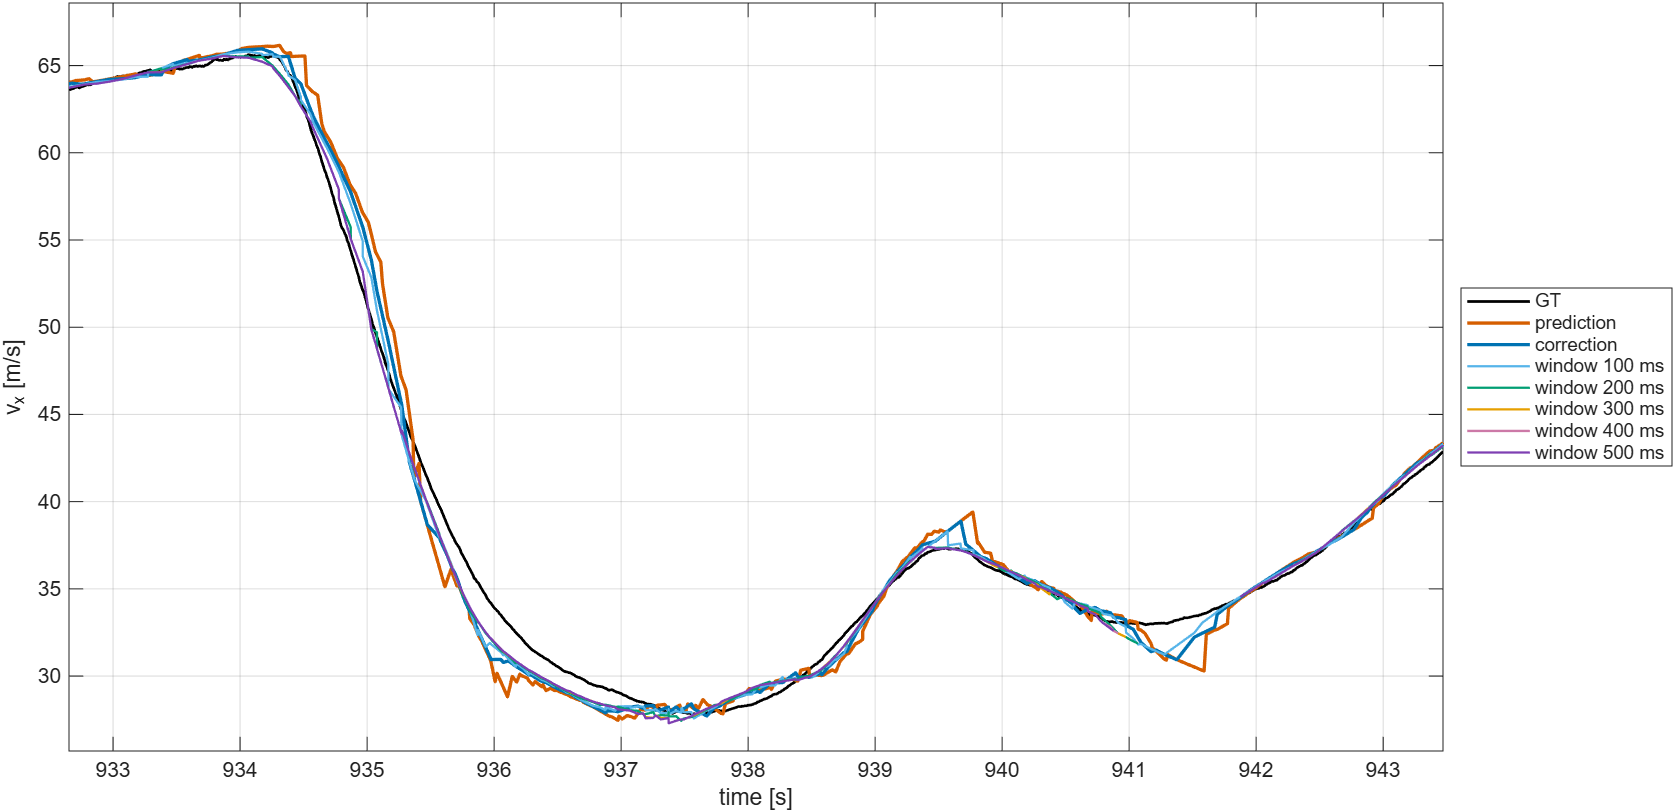
\includegraphics[width=0.76\textwidth]{figures/ch6/rts_lag_radar_corner.png}}
    \caption{Speed of the opponent estimated with different windows, all the sensors.}
    \label{fig:rts_lag_radar}
\end{figure}

The RMSE and the maneuver delay as a function of the window length are shown in
Fig.~\ref{fig:rts_metrics_radar} and reported in Table~\ref{tab:rts_radar}. With all the
sensors, increasing the window improves the estimate up to about 200--\SI{300}{ms}, beyond
which the gain saturates. With respect to the filtered estimate, the global RMSE decreases
by \SI{31}{\percent} and the local one by \SI{35}{\percent}. The saturation is due to the
fact that the forward filter already has a direct measurement of the speed, i.e.\ the
range rate of the RaDAR. The filter is therefore not very uncertain and, as discussed in
Section~\ref{subsec:rts_backward}, it does not need many future measurements. The median
maneuver delay moves from $+19$\,ms for the filtered estimate to about \SI{-62}{ms} for
windows longer than about \SI{180}{ms}, i.e.\ the smoothed estimate starts the maneuver
slightly before the ground truth. This anticipation is a direct consequence of the
backward pass. The future measurements that reveal the maneuver are spread backward over
the window, so that the estimate starts moving towards the new state before the maneuver
actually starts.

\begin{figure}[!htbp]
    \centering
    \subfloat[RMSE of the speed]{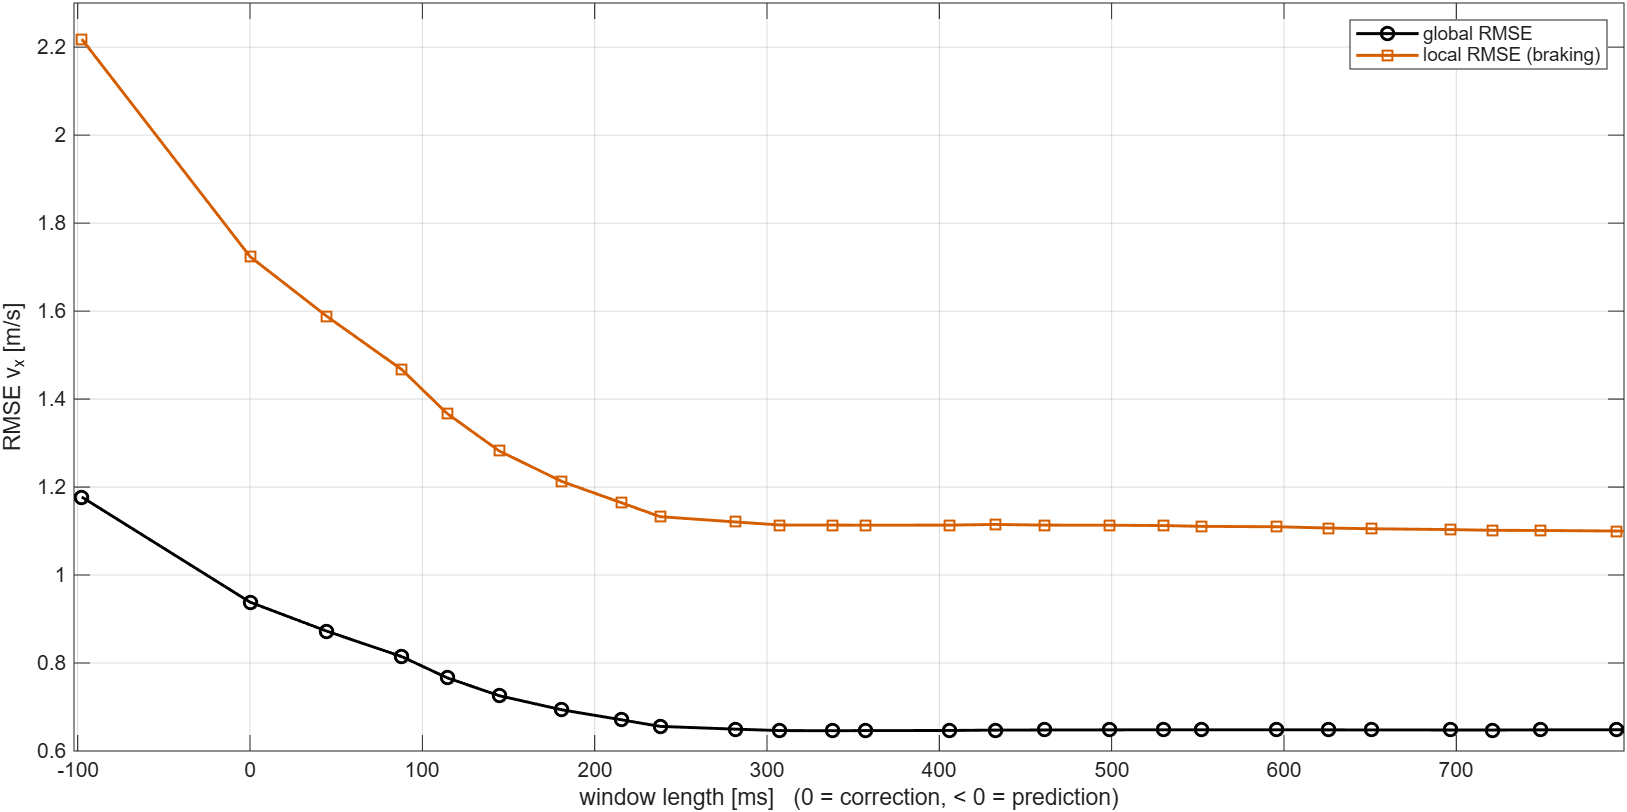
\includegraphics[width=0.76\textwidth]{figures/ch6/rts_rmse_radar.png}}\\
    \subfloat[Maneuver delay]{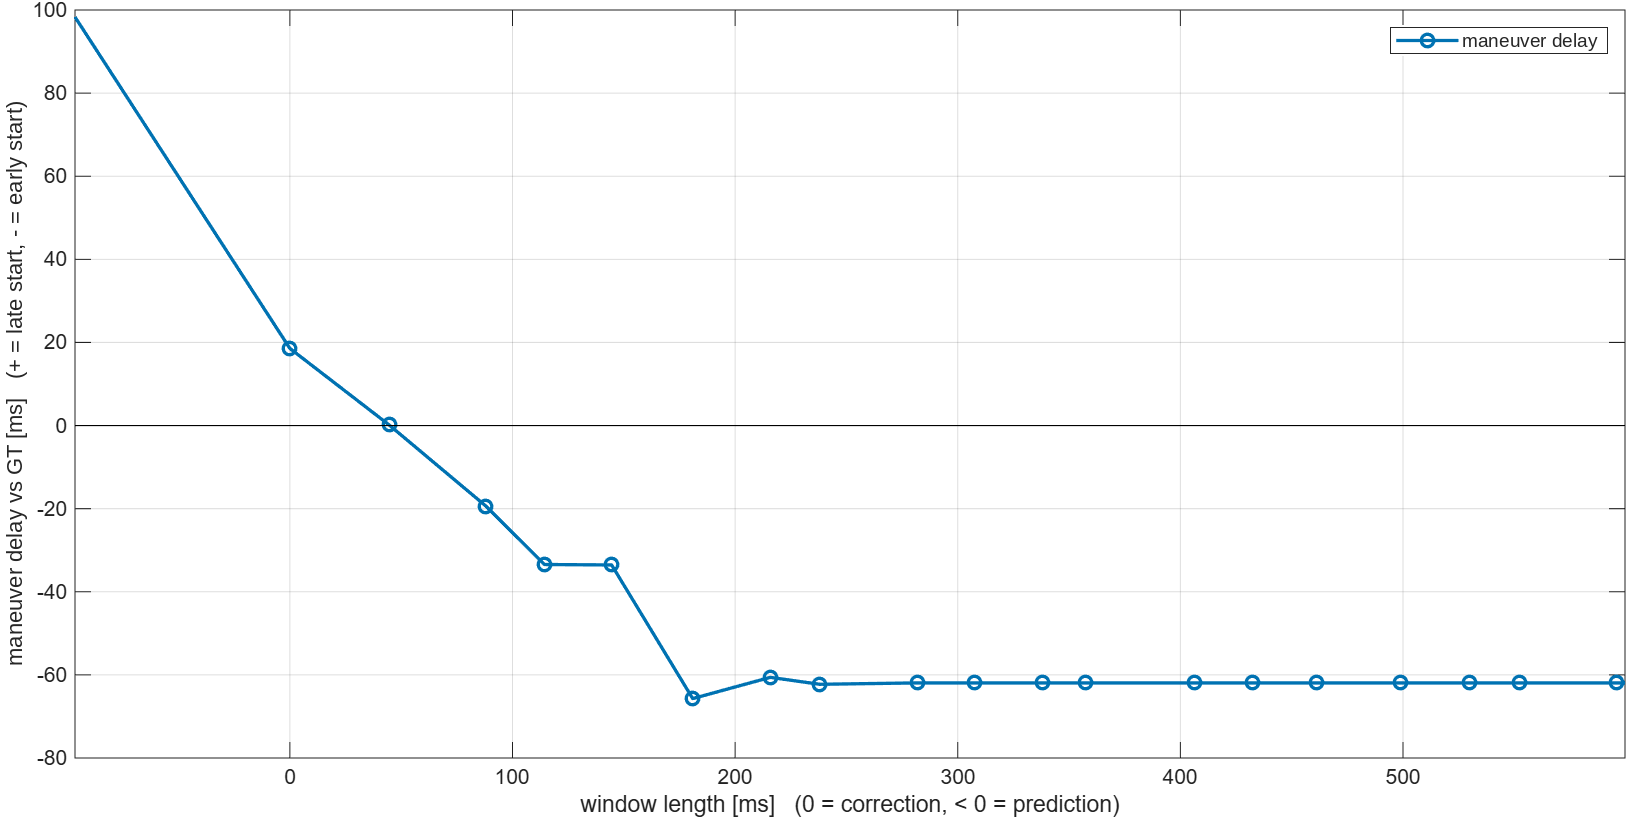
\includegraphics[width=0.76\textwidth]{figures/ch6/rts_delay_radar.png}}
    \caption{RMSE of the speed and maneuver delay as a function of the window length, all the
    sensors.}
    \label{fig:rts_metrics_radar}
\end{figure}

\begin{table}[!htbp]
\centering
\small
\begin{tabular}{rccccc}
\toprule
Window & \multicolumn{2}{c}{Global RMSE} & \multicolumn{2}{c}{Local RMSE} & Maneuver delay \\
\cmidrule(lr){2-3}\cmidrule(lr){4-5}
[ms] & [m/s] & $\Delta$ [\%] & [m/s] & $\Delta$ [\%] & [ms] \\
\midrule
  $-98$ & 1.177 & $+25.5$ & 2.218 & $+28.7$ & $+99$ \\
      0 & 0.938 & -- & 1.724 & -- & $+19$ \\
     88 & 0.815 & $-13.1$ & 1.467 & $-14.9$ & $-19$ \\
    145 & 0.726 & $-22.6$ & 1.282 & $-25.6$ & $-34$ \\
    216 & 0.671 & $-28.5$ & 1.164 & $-32.5$ & $-61$ \\
    308 & 0.646 & $-31.1$ & 1.114 & $-35.4$ & $-62$ \\
    406 & 0.647 & $-31.0$ & 1.113 & $-35.4$ & $-62$ \\
    499 & 0.648 & $-30.9$ & 1.113 & $-35.4$ & $-62$ \\
    697 & 0.648 & $-30.9$ & 1.103 & $-36.0$ & $-62$ \\
   1015 & 0.651 & $-30.6$ & 1.103 & $-36.0$ & $-62$ \\
\bottomrule
\end{tabular}
\caption{RMSE of the speed and median maneuver delay as a function of the window length, all the sensors. $\Delta$ is the variation with respect to the filtered estimate.}
\label{tab:rts_radar}
\end{table}

\FloatBarrier
\subsection*{Without Speed Measurements}
\label{subsec:rts_radar}

When the direct measurement of the speed is removed, i.e.\ without the RaDAR, the result
becomes more interesting. The speed is reconstructed from the positions only, the forward
filter is more uncertain, and the smoother corrects more. Fig.~\ref{fig:rts_lag_noradar}
shows that, in this case, the prediction and the correction lag behind the ground truth
more evidently, and the smoothed estimates obtained with the different windows are now
clearly separated. The longer the window, the earlier the smoothed estimate follows the
braking, until, for the longest windows, it starts the maneuver before the ground truth.

\begin{figure}[!htbp]
    \centering
    \subfloat[Braking]{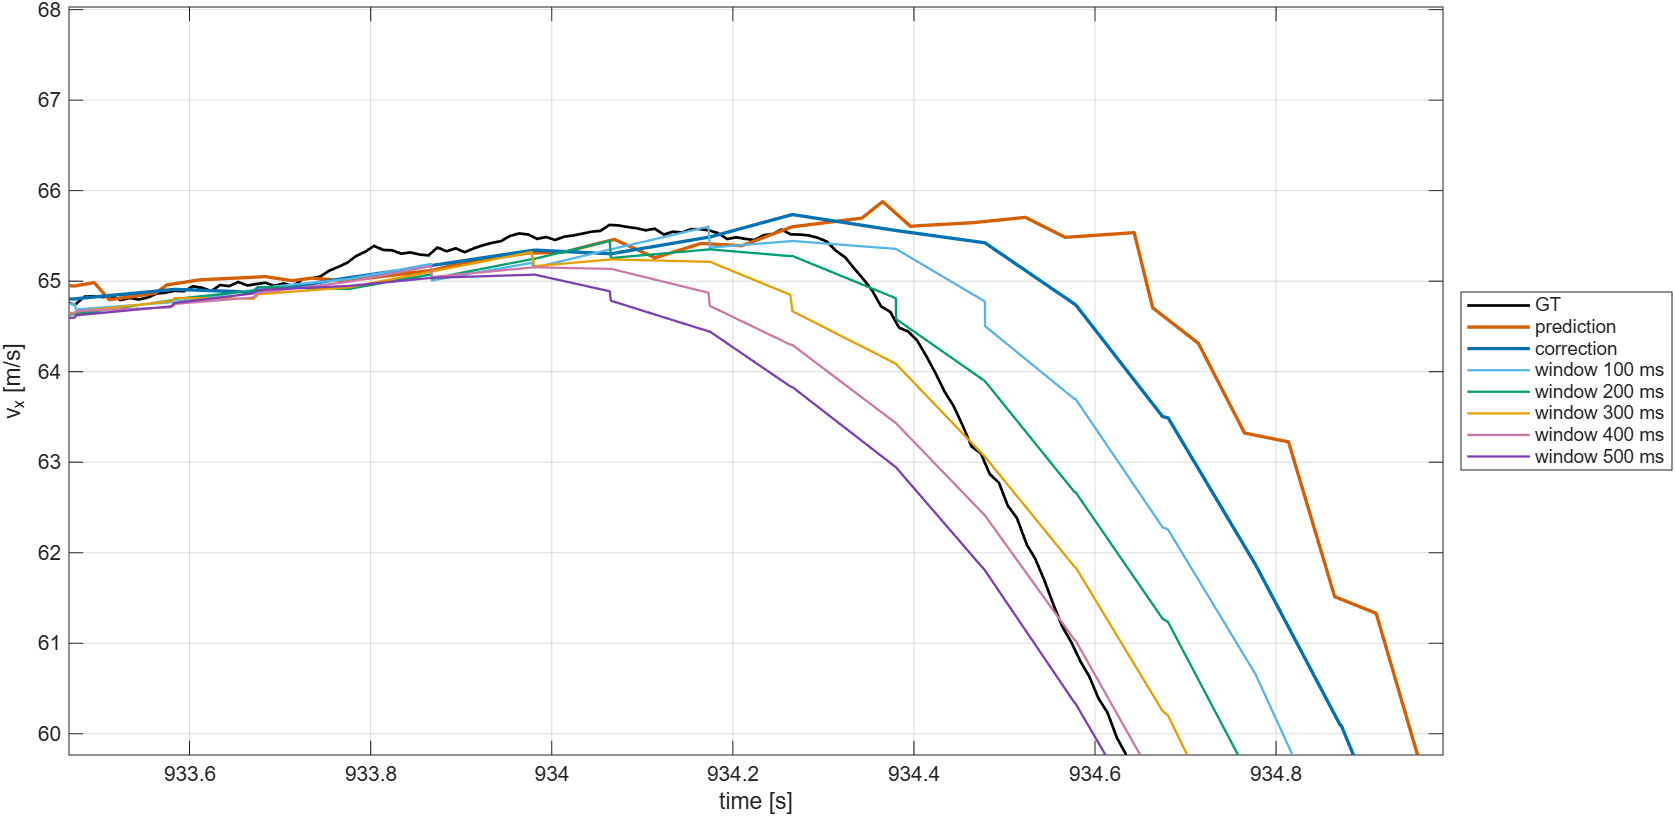
\includegraphics[width=0.76\textwidth]{figures/ch6/rts_lag_noradar_braking.png}}\\
    \subfloat[Corner]{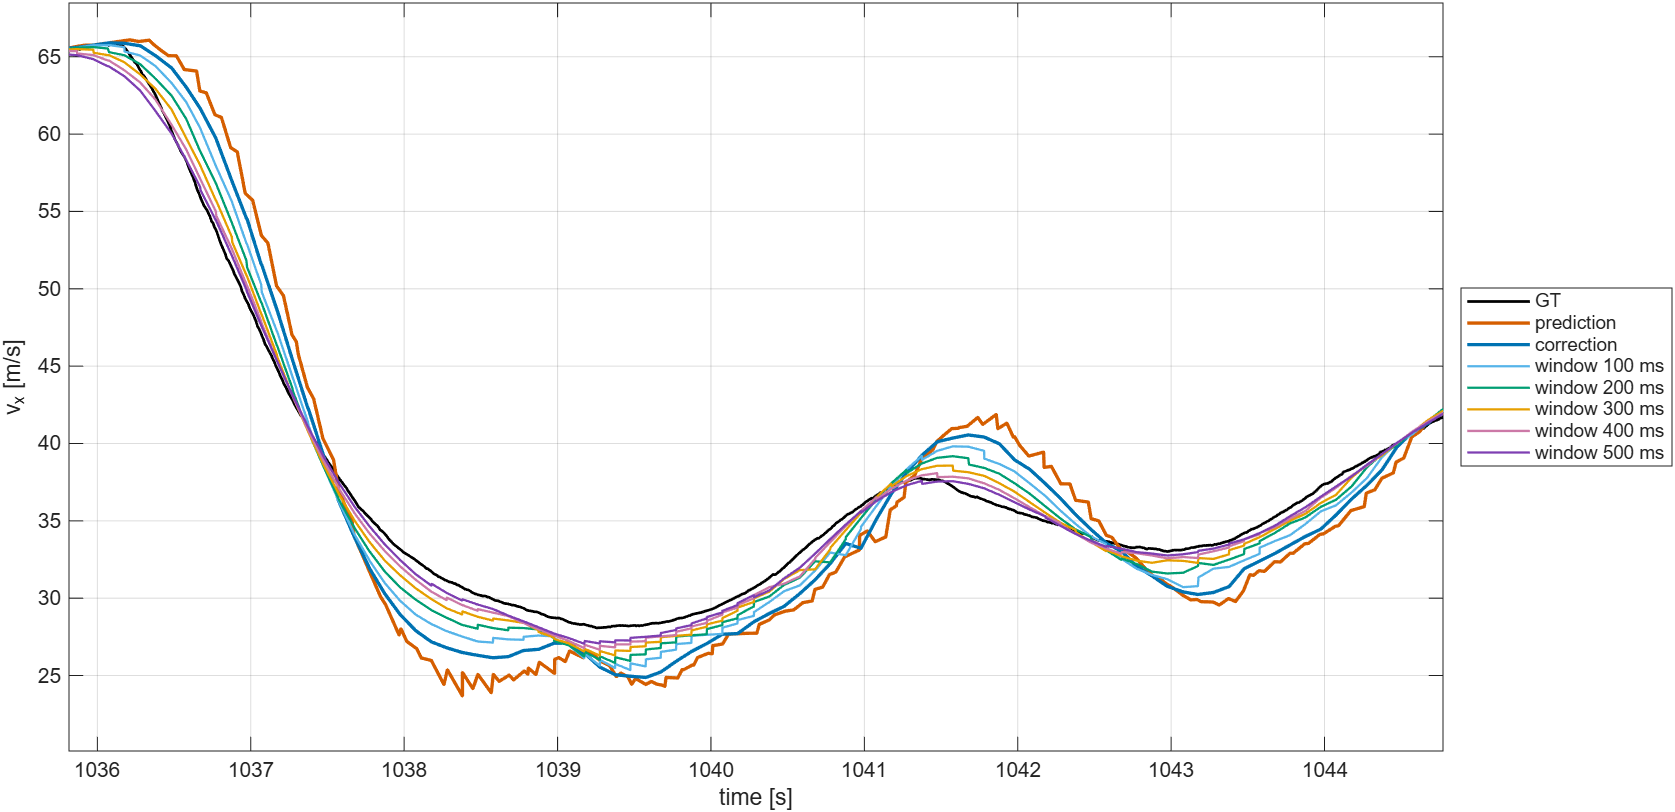
\includegraphics[width=0.76\textwidth]{figures/ch6/rts_lag_noradar_corner.png}}
    \caption{Speed of the opponent estimated with different windows, without the RaDAR.}
    \label{fig:rts_lag_noradar}
\end{figure}

\begin{figure}[!htbp]
    \centering
    \subfloat[RMSE of the speed]{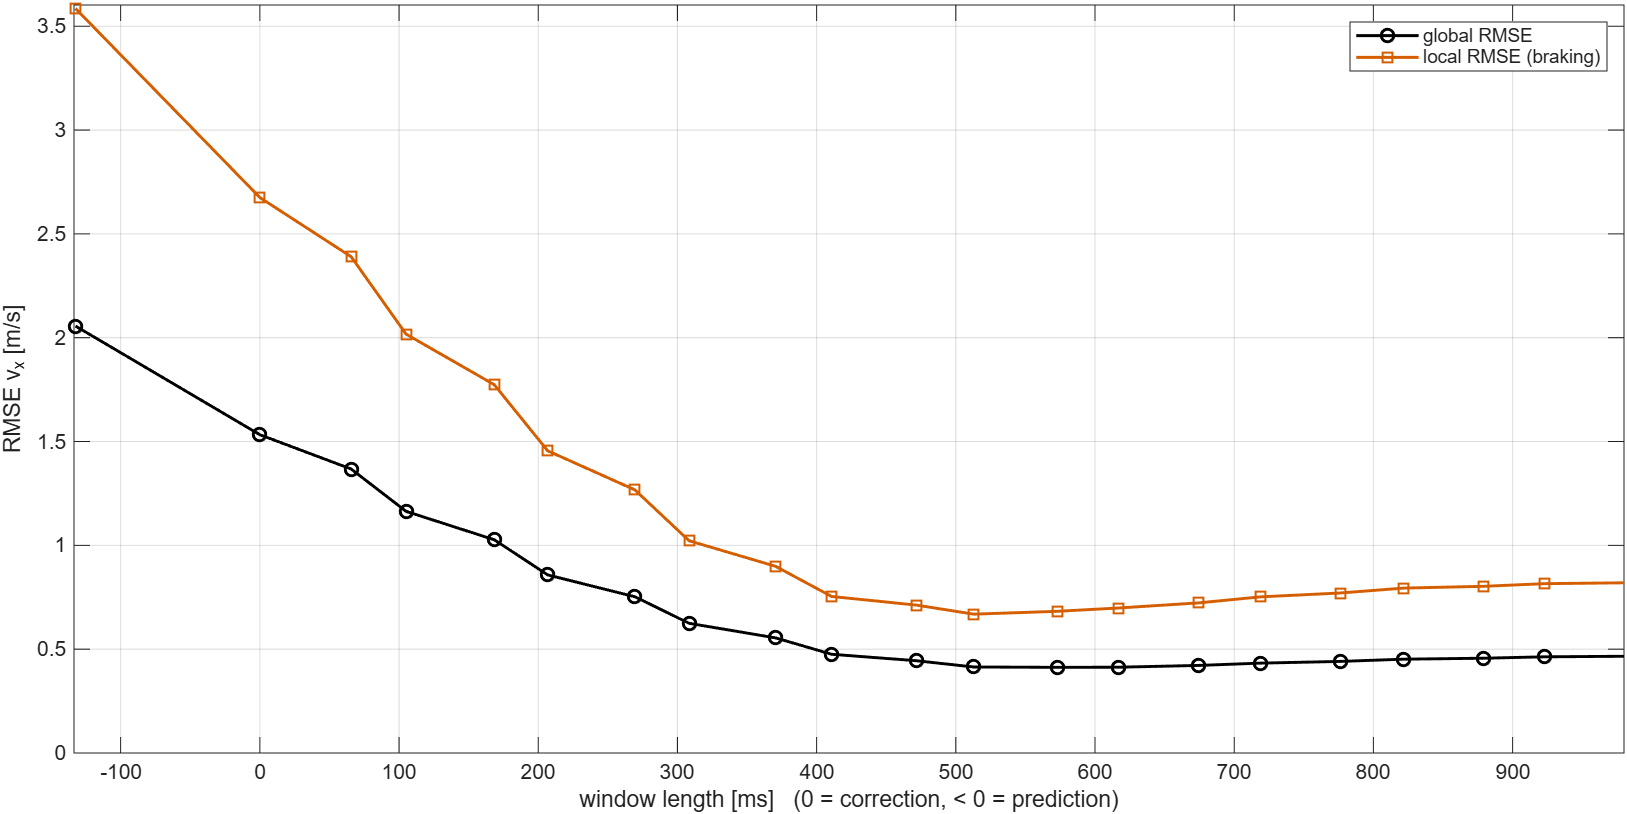
\includegraphics[width=0.76\textwidth]{figures/ch6/rts_rmse_noradar.png}}\\
    \subfloat[Maneuver delay]{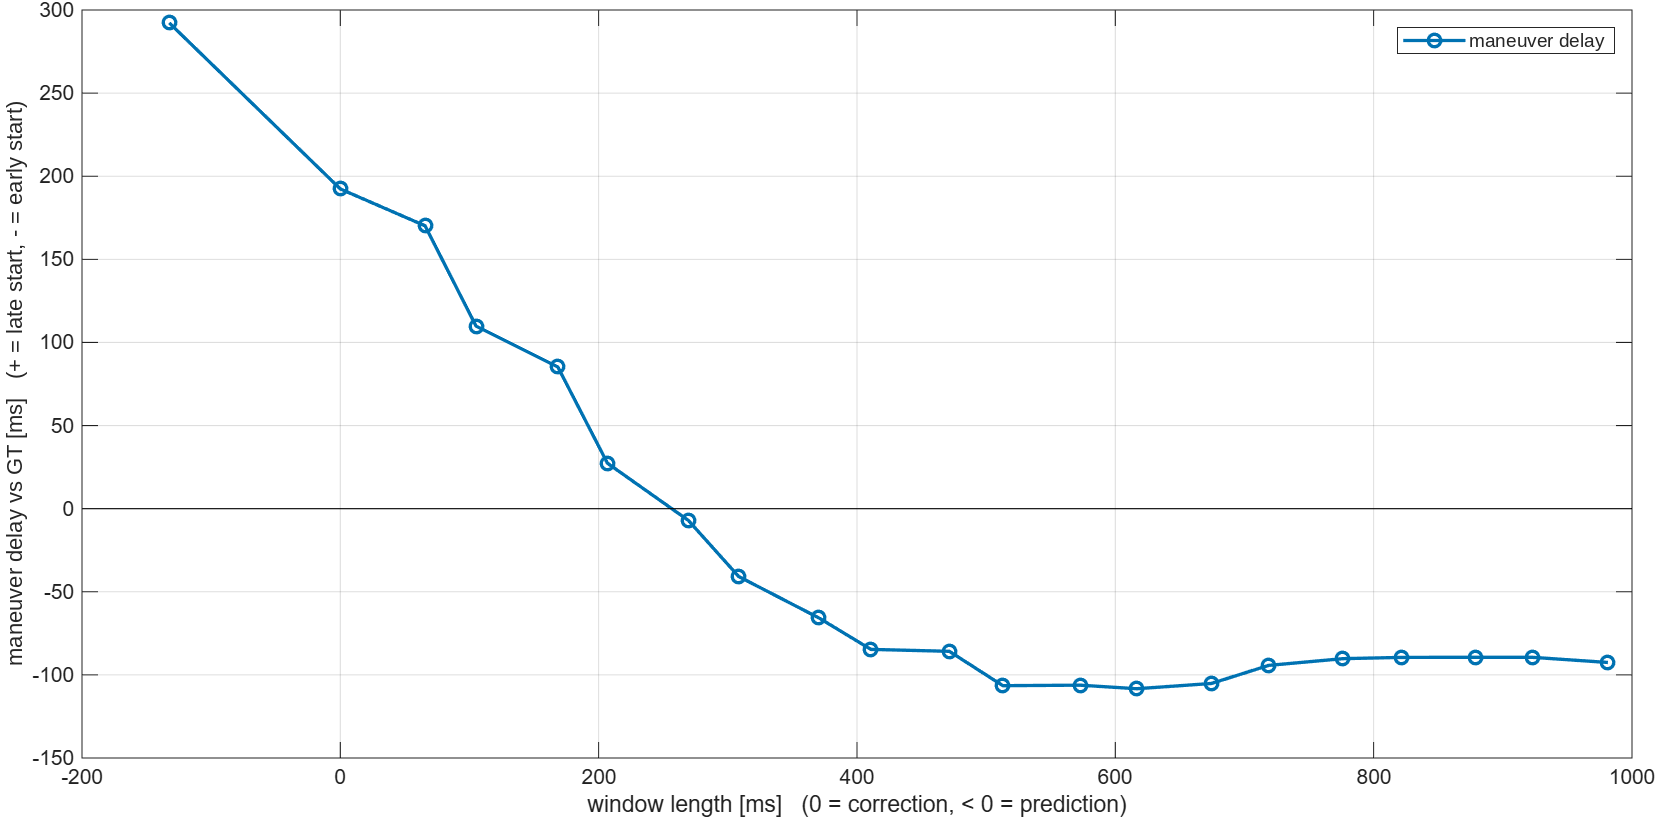
\includegraphics[width=0.76\textwidth]{figures/ch6/rts_delay_noradar.png}}
    \caption{RMSE of the speed and maneuver delay as a function of the window length, without
    the RaDAR.}
    \label{fig:rts_metrics_noradar}
\end{figure}

The results without the RaDAR are reported in Table~\ref{tab:rts_noradar}. The filtered
estimate is less accurate than with all the sensors, with a global RMSE of
\SI{1.533}{m/s} against \SI{0.938}{m/s}, and it starts the maneuvers later, with a median
maneuver delay of $+192$\,ms. Enlarging the window, the future information available to
the smoother increases and, since the forward filter is more uncertain, the smoother
corrects more. The global RMSE keeps decreasing up to about 500--\SI{600}{ms}, with a
reduction of \SI{73}{\percent}. The larger correction, however, also leads to anticipating
the maneuvers. The median maneuver delay becomes negative beyond about \SI{270}{ms}, and
it moves from \SI{-7}{ms} at \SI{269}{ms} to \SI{-41}{ms} at \SI{308}{ms}, \SI{-85}{ms} at
\SI{411}{ms} and \SI{-106}{ms} at \SI{513}{ms}, i.e.\ the effect grows as the window is
enlarged. As shown by the local RMSE, computed isolating the braking maneuvers, this
anticipation eventually degrades the estimate. The local RMSE reaches its minimum of
\SI{0.669}{m/s} at about \SI{500}{ms} and then starts increasing, up to \SI{0.820}{m/s} at
\SI{981}{ms}, i.e.\ beyond this point anticipating the maneuver increases the error.

\begin{table}[!htbp]
\centering
\small
\begin{tabular}{rccccc}
\toprule
Window & \multicolumn{2}{c}{Global RMSE} & \multicolumn{2}{c}{Local RMSE} & Maneuver delay \\
\cmidrule(lr){2-3}\cmidrule(lr){4-5}
[ms] & [m/s] & $\Delta$ [\%] & [m/s] & $\Delta$ [\%] & [ms] \\
\midrule
 $-132$ & 2.056 & $+34.1$ & 3.585 & $+34.0$ & $+292$ \\
      0 & 1.533 & -- & 2.675 & -- & $+192$ \\
    105 & 1.164 & $-24.1$ & 2.017 & $-24.6$ & $+110$ \\
    207 & 0.858 & $-44.0$ & 1.455 & $-45.6$ & $+27$ \\
    308 & 0.625 & $-59.2$ & 1.022 & $-61.8$ & $-41$ \\
    411 & 0.476 & $-68.9$ & 0.754 & $-71.8$ & $-85$ \\
    513 & 0.414 & $-73.0$ & 0.669 & $-75.0$ & $-106$ \\
    617 & 0.413 & $-73.1$ & 0.698 & $-73.9$ & $-108$ \\
    719 & 0.433 & $-71.8$ & 0.752 & $-71.9$ & $-94$ \\
    821 & 0.452 & $-70.5$ & 0.794 & $-70.3$ & $-89$ \\
    981 & 0.466 & $-69.6$ & 0.820 & $-69.3$ & $-93$ \\
\bottomrule
\end{tabular}
\caption{RMSE of the speed and median maneuver delay as a function of the window length, without the RaDAR. $\Delta$ is the variation with respect to the filtered estimate.}
\label{tab:rts_noradar}
\end{table}

\FloatBarrier
\subsection*{Comparison}
\label{subsec:rts_comparison}

Overall, the quality of the estimate of the speed improves in both cases, which justifies
the idea of using an acausal approach to improve the estimate of the state of the
opponent. The two cases are compared in Table~\ref{tab:rts_radar_noradar}.

\begin{table}[!htbp]
\centering
\small
\begin{tabular}{rcccccc}
\toprule
Window & \multicolumn{2}{c}{Global RMSE [m/s]} & \multicolumn{2}{c}{Local RMSE [m/s]} & \multicolumn{2}{c}{Maneuver delay [ms]} \\
\cmidrule(lr){2-3}\cmidrule(lr){4-5}\cmidrule(lr){6-7}
[ms] & RaDAR & No RaDAR & RaDAR & No RaDAR & RaDAR & No RaDAR \\
\midrule
$\approx -100$  & 1.177 & 2.056 & 2.218 & 3.585 & $+99$ & $+292$ \\
0               & 0.938 & 1.533 & 1.724 & 2.675 & $+19$ & $+192$ \\
$\approx 100$   & 0.815 & 1.164 & 1.467 & 2.017 & $-19$ & $+110$ \\
$\approx 200$   & 0.671 & 0.858 & 1.164 & 1.455 & $-61$ & $+27$ \\
$\approx 300$   & 0.646 & 0.625 & 1.114 & 1.022 & $-62$ & $-41$ \\
$\approx 400$   & 0.647 & 0.476 & 1.113 & 0.754 & $-62$ & $-85$ \\
$\approx 500$   & 0.648 & 0.414 & 1.113 & 0.669 & $-62$ & $-106$ \\
\bottomrule
\end{tabular}
\caption{RMSE of the speed and median maneuver delay as a function of the window length, with and
without the RaDAR.}
\label{tab:rts_radar_noradar}
\end{table}

The window length is fixed at about \SI{300}{ms} as a compromise between the two cases.
With the RaDAR, the improvement saturates at about \SI{300}{ms}, so that a longer window
brings no further benefit. Without it, the RMSE keeps decreasing with longer windows, but
the anticipation of the maneuvers grows with the window, and beyond about \SI{500}{ms} the
local RMSE increases again. A window of \SI{300}{ms} therefore keeps the anticipation
limited in both cases, at the cost of a higher RMSE than the minimum reachable without the
RaDAR.

Fixing the window at \SI{300}{ms}, Fig.~\ref{fig:rts_radar_noradar}
shows the comparison of the speed and of the acceleration estimated with and without the
RaDAR measurements. The orange lines are the smoothed (solid) and the causal (dashed)
estimates with the RaDAR measurements, while the blue ones are the same estimates without
the RaDAR measurements. As shown in the figure, in both cases the quality of the estimate
of the speed, and also of the acceleration, improves significantly.

\begin{figure}[H]
    \centering
    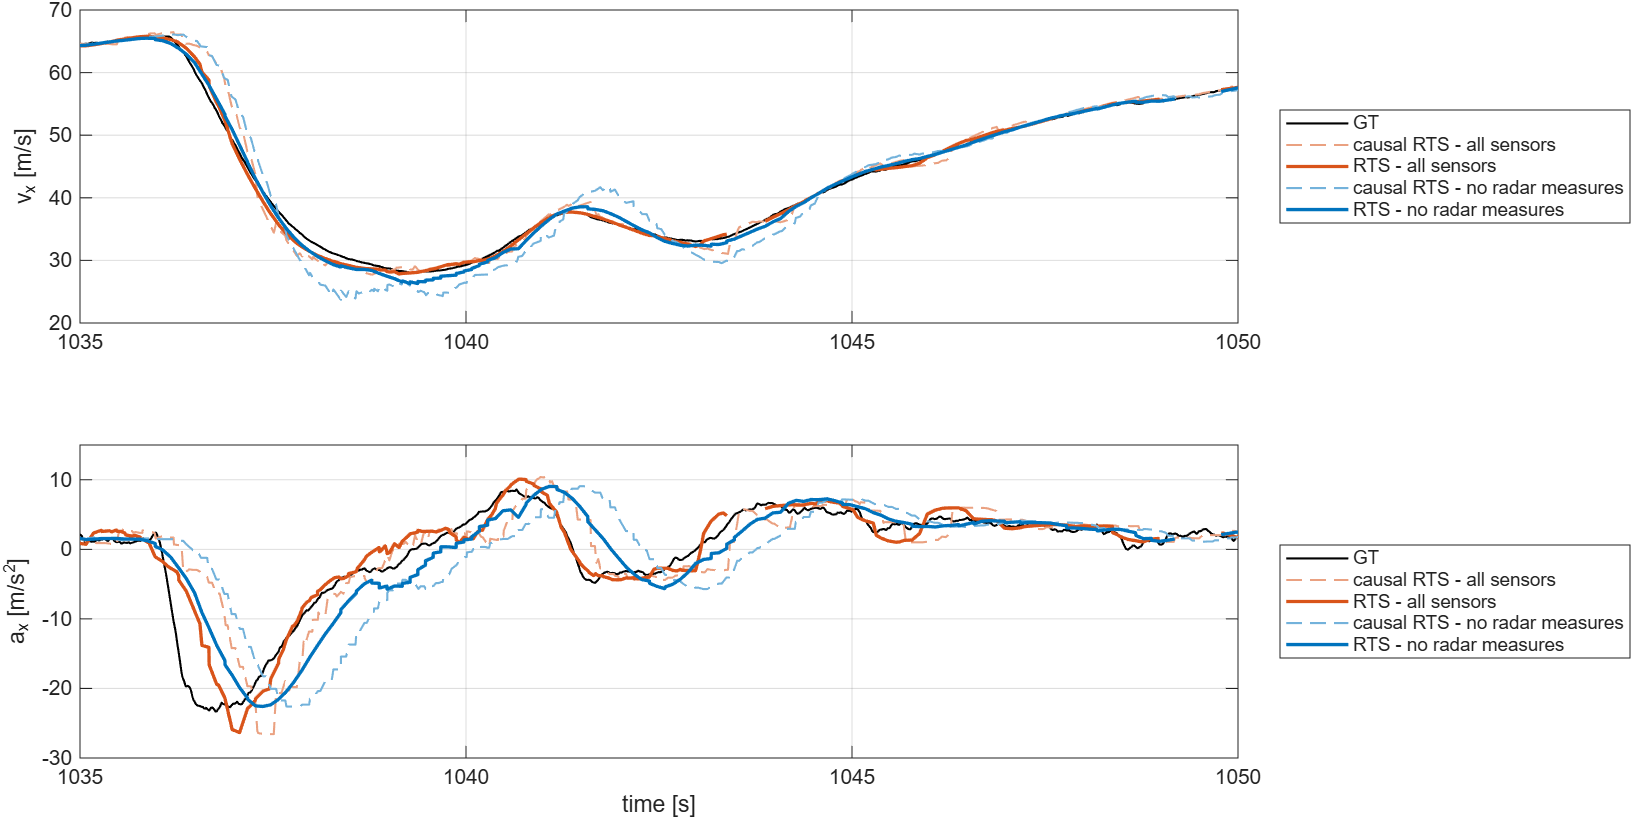
\includegraphics[width=0.85\textwidth]{figures/ch6/rts_radar_vs_noradar.png}
    \caption{Speed and acceleration estimated with and without the RaDAR, window of
    \SI{300}{ms}.}
    \label{fig:rts_radar_noradar}
\end{figure}

At \SI{300}{ms}, the smoothed estimate without the RaDAR reaches a global RMSE of
\SI{0.625}{m/s} and a local one of \SI{1.022}{m/s}, against \SI{0.646}{m/s} and
\SI{1.114}{m/s} with all the sensors. The most important result is therefore that, even in
the absence of direct measurements of the speed, the smoother provides a reliable estimate
of the speed of the opponent.

% =====================================================================
\section{Combination with the Q Feed-Forward}
\label{sec:rts_qff}

\TODO{Combination of the RTS smoother with the feed-forward process noise of
Chapter~\ref{ch:qff}. The smoother in series with the feed-forward approach could reduce
the effect of the noise of the jerk estimate and of the false activations of the maneuver
flag. Formulation, implementation and results.}

\chapter{Experimental Results}
\label{ch:results}

\TODO{}

\chapter{Conclusions and Future Work}
\label{ch:conclusions}

\TODO{}


%-------------------------------------------------------------------------
%	BIBLIOGRAPHY (to be enabled when the first citations are added)
%-------------------------------------------------------------------------
% \addtocontents{toc}{\vspace{2em}}
% \bibliography{Thesis_bibliography}

%-------------------------------------------------------------------------
%	APPENDICES
%-------------------------------------------------------------------------
\cleardoublepage
\addtocontents{toc}{\vspace{2em}}
\appendix
\refstepcounter{chapter}
\chapter*{Appendix A}
\addcontentsline{toc}{chapter}{Appendix A}
\markboth{Appendix A}{Appendix A}
\label{app:process_noise}

Starting from the Jacobian $\mathbf{A}$ of~\eqref{eq:tt_A}, the matrix exponential is
\begin{equation}
    \renewcommand{\arraystretch}{1.6}
    e^{\mathbf{A}\tau} =
    \begin{bmatrix}
        1 & 0 & \tau\cos\psi - \tfrac{1}{2}\kappa v\tau^2\sin\psi
          & \tfrac{1}{2}\tau^2\cos\psi - \tfrac{1}{6}\kappa v\tau^3\sin\psi & -v\tau\sin\psi \\
        0 & 1 & \tau\sin\psi + \tfrac{1}{2}\kappa v\tau^2\cos\psi
          & \tfrac{1}{2}\tau^2\sin\psi + \tfrac{1}{6}\kappa v\tau^3\cos\psi & \phantom{-}v\tau\cos\psi \\
        0 & 0 & 1 & \tau & 0 \\
        0 & 0 & 0 & 1 & 0 \\
        0 & 0 & \kappa\tau & \tfrac{1}{2}\kappa\tau^2 & 1
    \end{bmatrix}.
    \label{eq:app_exp}
\end{equation}
and~\eqref{eq:tt_Q_def}, with $\mathbf{G}$ and $\mathbf{Q}_c$ of~\eqref{eq:tt_noise}, gives
\begin{equation}
    \mathbf{Q}_k =
    \begin{bmatrix}
        q_{11} & q_{12} & 0      & q_{14} & q_{15} \\
        q_{12} & q_{22} & 0      & q_{24} & q_{25} \\
        0      & 0      & q_{33} & q_{34} & 0      \\
        q_{14} & q_{24} & q_{34} & q_{44} & q_{45} \\
        q_{15} & q_{25} & 0      & q_{45} & q_{55}
    \end{bmatrix},
    \label{eq:app_Q}
\end{equation}
\begin{equation}
    \renewcommand{\arraystretch}{2}
    \begin{aligned}
        q_{11} &= \tfrac{1}{3}\,q_\kappa v^4 \sin^2\psi\,\Delta t^3, &
        q_{12} &= -\tfrac{1}{3}\,q_\kappa v^4 \sin\psi\cos\psi\,\Delta t^3, \\
        q_{22} &= \tfrac{1}{3}\,q_\kappa v^4 \cos^2\psi\,\Delta t^3, &
        q_{14} &= \tfrac{1}{6}\,q_a \cos\psi\,\Delta t^3, \\
        q_{24} &= \tfrac{1}{6}\,q_a \sin\psi\,\Delta t^3, &
        q_{15} &= -\tfrac{1}{2}\,q_\kappa v^3 \sin\psi\,\Delta t^2, \\
        q_{25} &= \tfrac{1}{2}\,q_\kappa v^3 \cos\psi\,\Delta t^2, &
        q_{33} &= \tfrac{1}{3}\,q_a\,\Delta t^3, \\
        q_{34} &= \tfrac{1}{2}\,q_a\,\Delta t^2, &
        q_{44} &= q_a\,\Delta t, \\
        q_{45} &= \tfrac{1}{6}\,\kappa\,q_a\,\Delta t^3, &
        q_{55} &= q_\kappa v^2\,\Delta t.
    \end{aligned}
    \label{eq:app_Q_elements}
\end{equation}

\refstepcounter{chapter}
\chapter*{Appendix B}
\addcontentsline{toc}{chapter}{Appendix B}
\markboth{Appendix B}{Appendix B}
\label{app:lidar}

\begin{table}[H]
\centering
\setlength{\tabcolsep}{1.6pt}
\resizebox{\textwidth}{!}{%
\begin{tabular}{lccccc|ccccccccc}
\toprule
 & \multicolumn{5}{c|}{Rear, $|x_{\mathrm{rel}}|$ [m]} & \multicolumn{9}{c}{Front, $x_{\mathrm{rel}}$ [m]} \\
Session & 60--50 & 50--40 & 40--30 & 30--20 & 20--10 & 10--20 & 20--30 & 30--40 & 40--50 & 50--60 & 60--70 & 70--80 & 80--90 & 90--100 \\
\midrule
07/26\_TUM & -- & 0.67 & 0.42 & 0.20 & 0.08 & 0.05 & 0.19 & 0.09 & 0.11 & 0.17 & 0.18 & 0.21 & 0.23 & 0.25 \\
08/03\_Kinetiz & 0.38 & 0.30 & 0.32 & 0.15 & 0.16 & 0.18 & 0.16 & 0.15 & 0.15 & 0.15 & 0.20 & 0.21 & 0.24 & 0.21 \\
10/12 (EVA+LIVIA) & -- & 0.28 & 0.22 & 0.09 & 0.04 & 0.04 & 0.04 & 0.17 & 0.06 & 0.07 & 0.09 & 0.08 & 0.08 & 0.16 \\
10/13 (EVA+LIVIA) & 0.23 & 0.24 & -- & -- & -- & -- & -- & 0.17 & 0.17 & 0.10 & 0.07 & 0.11 & 0.21 & 0.19 \\
10/14\_eva & -- & 0.15 & 0.12 & 0.14 & 0.53$^{*}$ & 0.10 & 0.08 & 0.08 & 0.10 & 0.10 & 0.12 & 0.16 & 0.15 & 0.13 \\
10/14-02 (EVA+LIVIA) & -- & 0.38 & 0.21 & 0.12 & 0.07 & 0.08 & 0.08 & 0.11 & 0.12 & 0.08 & 0.12 & 0.13 & -- & -- \\
10/14-04 (EVA) & -- & -- & 0.17 & 0.10 & 0.08 & 0.08 & 0.14 & 0.15 & 0.19 & 0.14 & 0.13 & 0.13 & 0.11 & 0.10 \\
10/16 (EVA+LIVIA) & -- & -- & 0.29 & 0.18 & 0.20 & 0.06 & 0.07 & 0.10 & 0.10 & 0.09 & 0.11 & 0.14 & 0.15 & 0.10 \\
\bottomrule
\end{tabular}}
\par\vspace{2pt}{\footnotesize $^{*}$ 10/14\_eva: at 10--20\,m behind the opponent is almost on the ego axis (median $|y_{\mathrm{rel}}|\approx2$\,m, rear blind strip); without the samples with $|y_{\mathrm{rel}}|<2$\,m: $\sigma_x=0.12$\,m, $\sigma_y=0.18$\,m.}
\caption{LiDAR Clustering: standard deviation of the longitudinal error $\sigma_x$ [m] vs $x_{\mathrm{rel}}$ (10\,m bins).}
\label{tab:clust_sx}
\end{table}

\begin{table}[H]
\centering
\setlength{\tabcolsep}{1.6pt}
\resizebox{\textwidth}{!}{%
\begin{tabular}{lccccc|ccccccccc}
\toprule
 & \multicolumn{5}{c|}{Rear, $|x_{\mathrm{rel}}|$ [m]} & \multicolumn{9}{c}{Front, $x_{\mathrm{rel}}$ [m]} \\
Session & 60--50 & 50--40 & 40--30 & 30--20 & 20--10 & 10--20 & 20--30 & 30--40 & 40--50 & 50--60 & 60--70 & 70--80 & 80--90 & 90--100 \\
\midrule
07/26\_TUM & -- & 0.69 & 0.35 & 0.19 & 0.08 & 0.09 & 0.25 & 0.13 & 0.16 & 0.23 & 0.27 & 0.27 & 0.30 & 0.43 \\
08/03\_Kinetiz & 0.49 & 0.39 & 0.33 & 0.29 & 0.21 & 0.08 & 0.10 & 0.09 & 0.10 & 0.14 & 0.14 & 0.35 & 0.38 & 0.39 \\
10/12 (EVA+LIVIA) & -- & 0.33 & 0.20 & 0.11 & 0.08 & 0.05 & 0.06 & 0.09 & 0.11 & 0.15 & 0.19 & 0.23 & 0.31 & 0.54 \\
10/13 (EVA+LIVIA) & 0.51 & 0.44 & -- & -- & -- & -- & -- & 0.07 & 0.16 & 0.18 & 0.16 & 0.28 & 0.31 & 0.37 \\
10/14\_eva & -- & 0.17 & 0.18 & 0.31 & 0.47$^{*}$ & 0.10 & 0.11 & 0.09 & 0.13 & 0.13 & 0.19 & 0.25 & 0.21 & 0.28 \\
10/14-02 (EVA+LIVIA) & -- & 0.63 & 0.43 & 0.14 & 0.07 & 0.08 & 0.09 & 0.14 & 0.17 & 0.16 & 0.19 & 0.23 & -- & -- \\
10/14-04 (EVA) & -- & -- & 0.38 & 0.23 & 0.10 & 0.05 & 0.13 & 0.20 & 0.11 & 0.17 & 0.26 & 0.25 & 0.23 & 0.29 \\
10/16 (EVA+LIVIA) & -- & -- & 0.44 & 0.29 & 0.29 & 0.12 & 0.08 & 0.20 & 0.11 & 0.14 & 0.23 & 0.25 & 0.19 & 0.23 \\
\bottomrule
\end{tabular}}
\par\vspace{2pt}{\footnotesize $^{*}$ 10/14\_eva: at 10--20\,m behind the opponent is almost on the ego axis (median $|y_{\mathrm{rel}}|\approx2$\,m, rear blind strip); without the samples with $|y_{\mathrm{rel}}|<2$\,m: $\sigma_x=0.12$\,m, $\sigma_y=0.18$\,m.}
\caption{LiDAR Clustering: standard deviation of the lateral error $\sigma_y$ [m] vs $x_{\mathrm{rel}}$ (10\,m bins).}
\label{tab:clust_sy}
\end{table}

\begin{table}[H]
\centering
\setlength{\tabcolsep}{1.6pt}
\resizebox{\textwidth}{!}{%
\begin{tabular}{lccccc|ccccccccc}
\toprule
 & \multicolumn{5}{c|}{Rear, $|x_{\mathrm{rel}}|$ [m]} & \multicolumn{9}{c}{Front, $x_{\mathrm{rel}}$ [m]} \\
Session & 60--50 & 50--40 & 40--30 & 30--20 & 20--10 & 10--20 & 20--30 & 30--40 & 40--50 & 50--60 & 60--70 & 70--80 & 80--90 & 90--100 \\
\midrule
07/26\_TUM & -- & $+0.28$ & $+0.24$ & $+0.26$ & $+0.15$ & $+0.01$ & $0.00$ & $-0.01$ & $-0.04$ & $-0.08$ & $-0.09$ & $-0.08$ & $-0.13$ & $-0.19$ \\
08/03\_Kinetiz & $+0.30$ & $+0.29$ & $+0.27$ & $+0.24$ & $+0.13$ & $-0.01$ & $-0.01$ & $-0.03$ & $-0.14$ & $-0.16$ & $-0.20$ & $-0.29$ & $-0.28$ & $-0.23$ \\
10/12 (EVA+LIVIA) & -- & $+0.37$ & $+0.36$ & $+0.30$ & $+0.23$ & $+0.09$ & $+0.07$ & $+0.01$ & $+0.01$ & $-0.02$ & $-0.02$ & $0.00$ & $-0.05$ & $-0.06$ \\
10/13 (EVA+LIVIA) & $+0.30$ & -- & -- & -- & -- & -- & -- & $0.00$ & $+0.04$ & $-0.01$ & $0.00$ & $-0.03$ & $-0.08$ & $-0.11$ \\
10/14\_eva & $+0.34$ & $+0.36$ & $+0.30$ & $+0.26$ & $+0.24$ & $+0.04$ & $+0.02$ & $0.00$ & $+0.01$ & $-0.01$ & $-0.01$ & $-0.05$ & $-0.09$ & $-0.10$ \\
10/14-02 (EVA+LIVIA) & $+0.47$ & $+0.43$ & $+0.39$ & $+0.37$ & $+0.23$ & $+0.14$ & $+0.06$ & $0.00$ & $-0.01$ & $-0.03$ & $+0.09$ & $+0.08$ & $+0.05$ & -- \\
10/14-04 (EVA) & -- & -- & $+0.30$ & $+0.29$ & $+0.24$ & $+0.08$ & $+0.03$ & $+0.03$ & $0.00$ & $-0.04$ & $-0.04$ & $-0.01$ & $-0.07$ & $-0.10$ \\
10/16 (EVA+LIVIA) & $+0.43$ & $+0.40$ & $+0.37$ & $+0.33$ & $+0.28$ & $+0.04$ & $0.00$ & $+0.04$ & $-0.05$ & $-0.04$ & $-0.06$ & $-0.07$ & $-0.14$ & $-0.23$ \\
\bottomrule
\end{tabular}}
\caption{LiDAR PointPillars: mean longitudinal error $e_x$ [m] vs $x_{\mathrm{rel}}$ (10\,m bins). Reference offset removed.}
\label{tab:pp_ex}
\end{table}

\begin{table}[H]
\centering
\setlength{\tabcolsep}{4pt}\small
\begin{tabular}{lccccccccc}
\toprule
Session & \multicolumn{9}{c}{$|x_{\mathrm{rel}}|$ [m]} \\
\cmidrule(l){2-10}
 & 10--20 & 20--30 & 30--40 & 40--50 & 50--60 & 60--70 & 70--80 & 80--90 & 90--100 \\
\midrule
\multicolumn{10}{l}{\textit{Rear ($x_{\mathrm{rel}}<0$)}} \\
07/26\_TUM & 0.42 & 0.57 & 0.64 & 0.75 & 0.90 & 0.69 & 0.91 & 0.92 & 1.12 \\
08/03\_Kinetiz & 0.43 & 0.52 & 0.57 & 0.66 & 0.68 & 0.62 & 0.83 & 0.94 & 0.83 \\
10/12 (EVA+LIVIA) & 0.41 & 0.56 & 0.60 & 0.62 & 0.74 & 0.75 & 0.77 & 0.95 & 0.75 \\
10/13 (EVA+LIVIA) & -- & -- & 0.48 & 0.65 & 0.88 & 0.74 & 0.63 & 0.85 & 1.00 \\
10/14\_eva & 0.43 & 0.50 & 0.62 & 0.65 & 0.61 & 0.63 & 0.49 & -- & -- \\
10/14-02 (EVA+LIVIA) & 0.62 & 0.58 & 0.61 & 0.63 & 0.66 & 0.70 & 0.60 & 0.61 & 0.80 \\
10/14-04 (EVA) & 0.46 & 0.57 & 0.64 & 0.60 & 0.76 & -- & -- & -- & -- \\
10/16 (EVA+LIVIA) & 0.47 & 0.51 & 0.70 & 0.73 & 0.84 & 0.88 & 0.90 & 1.04 & 0.91 \\
\midrule
\multicolumn{10}{l}{\textit{Front ($x_{\mathrm{rel}}>0$)}} \\
07/26\_TUM & 0.45 & 0.45 & 0.52 & 0.57 & 0.63 & 0.65 & 0.62 & 0.77 & 0.71 \\
08/03\_Kinetiz & 0.52 & 0.53 & 0.53 & 0.53 & 0.54 & 0.59 & 0.68 & 0.82 & 0.82 \\
10/12 (EVA+LIVIA) & 0.39 & 0.51 & 0.54 & 0.62 & 0.63 & 0.68 & 0.69 & 0.80 & 0.76 \\
10/13 (EVA+LIVIA) & -- & -- & -- & 0.57 & 0.62 & 0.72 & 0.64 & 0.79 & 0.67 \\
10/14\_eva & 0.35 & 0.45 & 0.49 & 0.54 & 0.59 & 0.67 & 0.74 & 0.93 & 0.91 \\
10/14-02 (EVA+LIVIA) & 0.46 & 0.50 & 0.48 & 0.56 & 0.49 & 0.53 & 0.55 & 0.79 & 0.71 \\
10/14-04 (EVA) & -- & 0.32 & 0.42 & 0.53 & 0.52 & 0.48 & 0.48 & 0.73 & 0.66 \\
10/16 (EVA+LIVIA) & 0.69 & 0.57 & 0.53 & 0.63 & 0.75 & 0.83 & 0.91 & 0.86 & 0.63 \\
\bottomrule
\end{tabular}
\caption{RaDAR: standard deviation of the longitudinal error $\sigma_x$ [m] vs $|x_{\mathrm{rel}}|$ (10\,m bins).}
\label{tab:rad_sx}
\end{table}

\begin{table}[H]
\centering
\setlength{\tabcolsep}{4pt}\small
\begin{tabular}{lccccccccc}
\toprule
Session & \multicolumn{9}{c}{$|x_{\mathrm{rel}}|$ [m]} \\
\cmidrule(l){2-10}
 & 10--20 & 20--30 & 30--40 & 40--50 & 50--60 & 60--70 & 70--80 & 80--90 & 90--100 \\
\midrule
\multicolumn{10}{l}{\textit{Rear ($x_{\mathrm{rel}}<0$)}} \\
07/26\_TUM & $+0.31$ & $+0.06$ & $-0.16$ & $-0.16$ & $-0.17$ & $+0.17$ & $-0.16$ & $-0.05$ & $-0.11$ \\
08/03\_Kinetiz & $+0.56$ & $+0.10$ & $+0.22$ & $+0.05$ & $+0.19$ & $+0.20$ & $+0.21$ & $+0.12$ & $+0.13$ \\
10/12 (EVA+LIVIA) & $+0.29$ & $+0.18$ & $+0.25$ & $+0.21$ & $+0.49$ & $+0.40$ & $+0.34$ & $+0.47$ & $+0.15$ \\
10/13 (EVA+LIVIA) & -- & -- & $+0.20$ & $+0.20$ & $+0.14$ & $+0.30$ & $+0.35$ & $+0.16$ & $+0.20$ \\
10/14\_eva & $+0.58$ & $+0.25$ & $+0.12$ & $+0.17$ & $+0.24$ & $+0.50$ & $+0.19$ & -- & -- \\
10/14-02 (EVA+LIVIA) & $+0.35$ & $+0.35$ & $+0.30$ & $+0.35$ & $+0.35$ & $+0.55$ & $+0.74$ & $+0.60$ & $+0.64$ \\
10/14-04 (EVA) & $+0.82$ & $+0.59$ & $+0.34$ & $+0.51$ & $+0.49$ & -- & -- & -- & -- \\
10/16 (EVA+LIVIA) & $+0.84$ & $+0.76$ & $+0.56$ & $+0.59$ & $+0.48$ & $+0.73$ & $+0.64$ & $+0.42$ & $+0.51$ \\
\midrule
\multicolumn{10}{l}{\textit{Front ($x_{\mathrm{rel}}>0$)}} \\
07/26\_TUM & $-0.67$ & $-0.84$ & $-0.79$ & $-0.86$ & $-1.00$ & $-0.99$ & $-1.00$ & $-1.05$ & $-1.36$ \\
08/03\_Kinetiz & $-0.44$ & $-0.46$ & $-0.56$ & $-0.82$ & $-0.74$ & $-0.76$ & $-0.92$ & $-0.95$ & $-1.06$ \\
10/12 (EVA+LIVIA) & $-0.35$ & $-0.35$ & $-0.61$ & $-0.50$ & $-0.57$ & $-0.46$ & $-0.53$ & $-0.63$ & $-0.97$ \\
10/13 (EVA+LIVIA) & -- & -- & -- & $-0.63$ & $-0.52$ & $-0.47$ & $-0.64$ & $-0.80$ & $-0.98$ \\
10/14\_eva & $-1.33$ & $-0.86$ & $-0.83$ & $-0.68$ & $-0.73$ & $-0.67$ & $-0.67$ & $-0.65$ & $-1.00$ \\
10/14-02 (EVA+LIVIA) & $-0.50$ & $-0.36$ & $-0.63$ & $-0.67$ & $-0.76$ & $-0.53$ & $-0.41$ & $-0.53$ & $-0.81$ \\
10/14-04 (EVA) & -- & $-1.00$ & $-1.14$ & $-1.23$ & $-1.38$ & $-1.12$ & $-0.95$ & $-1.45$ & $-1.69$ \\
10/16 (EVA+LIVIA) & $-0.18$ & $-0.37$ & $-0.27$ & $-0.52$ & $-0.77$ & $-0.45$ & $-0.52$ & $-0.92$ & $-1.18$ \\
\bottomrule
\end{tabular}
\caption{RaDAR: mean longitudinal error $e_x$ [m] vs $|x_{\mathrm{rel}}|$ (10\,m bins). Reference offset removed.}
\label{tab:rad_ex}
\end{table}

\begin{table}[H]
\centering
\setlength{\tabcolsep}{4pt}\small
\resizebox{\textwidth}{!}{%
\begin{tabular}{lccccccccc|c}
\toprule
Session & \multicolumn{9}{c|}{$x_{\mathrm{rel}}$ [m]} & Trend \\
\cmidrule(lr){2-10}
 & 10--20 & 20--30 & 30--40 & 40--50 & 50--60 & 60--70 & 70--80 & 80--90 & 90--100 & [cm/m] \\
\midrule
07/26\_TUM & $+0.57$ & $-0.04$ & $-0.08$ & $-0.03$ & $+0.07$ & $+0.28$ & $+0.36$ & $+0.39$ & $+0.40$ & $+0.92$ \\
08/03\_Kinetiz & $+0.66$ & $+0.10$ & $-0.10$ & $-0.06$ & $+0.03$ & $+0.18$ & $+0.19$ & $+0.30$ & $+0.25$ & $+0.81$ \\
10/12 (EVA) & -- & $-0.25$ & $-0.25$ & $-0.03$ & $+0.14$ & $+0.46$ & $+0.53$ & $+0.55$ & $+0.62$ & $+1.41$ \\
10/13 (EVA) & -- & -- & $-0.20$ & $+0.15$ & $+0.23$ & $+0.39$ & $+0.44$ & $+0.44$ & $+0.52$ & $+0.70$ \\
10/14\_eva & $+0.29$ & $+0.25$ & $+0.01$ & $+0.10$ & $+0.21$ & $+0.37$ & $+0.44$ & $+0.46$ & $+0.59$ & $+1.14$ \\
10/14-02 (EVA+LIVIA) & $+1.16$ & $-0.03$ & $-0.12$ & $+0.03$ & $+0.22$ & $+0.43$ & $+0.57$ & $+0.60$ & $+0.60$ & $+1.49$ \\
10/14-04 (EVA) & $+0.70$ & $+0.23$ & $+0.05$ & $-0.11$ & $+0.14$ & $+0.46$ & $+0.53$ & $+0.52$ & $+0.57$ & $+1.20$ \\
10/16 (EVA+LIVIA) & $+0.43$ & $+0.20$ & $+0.17$ & $+0.07$ & $+0.22$ & $+0.39$ & $+0.44$ & $+0.47$ & $+0.47$ & $+0.94$ \\
\bottomrule
\end{tabular}}
\caption{Camera: mean longitudinal error $e_x$ [m] vs $x_{\mathrm{rel}}$ (10\,m bins, opponent
ahead). Reference offset removed. Trend: slope~\eqref{eq:macro_slope} of $e_x$ between 40 and 100\,m.}
\label{tab:cam_x}
\end{table}


\begin{figure}[H]
    \centering
    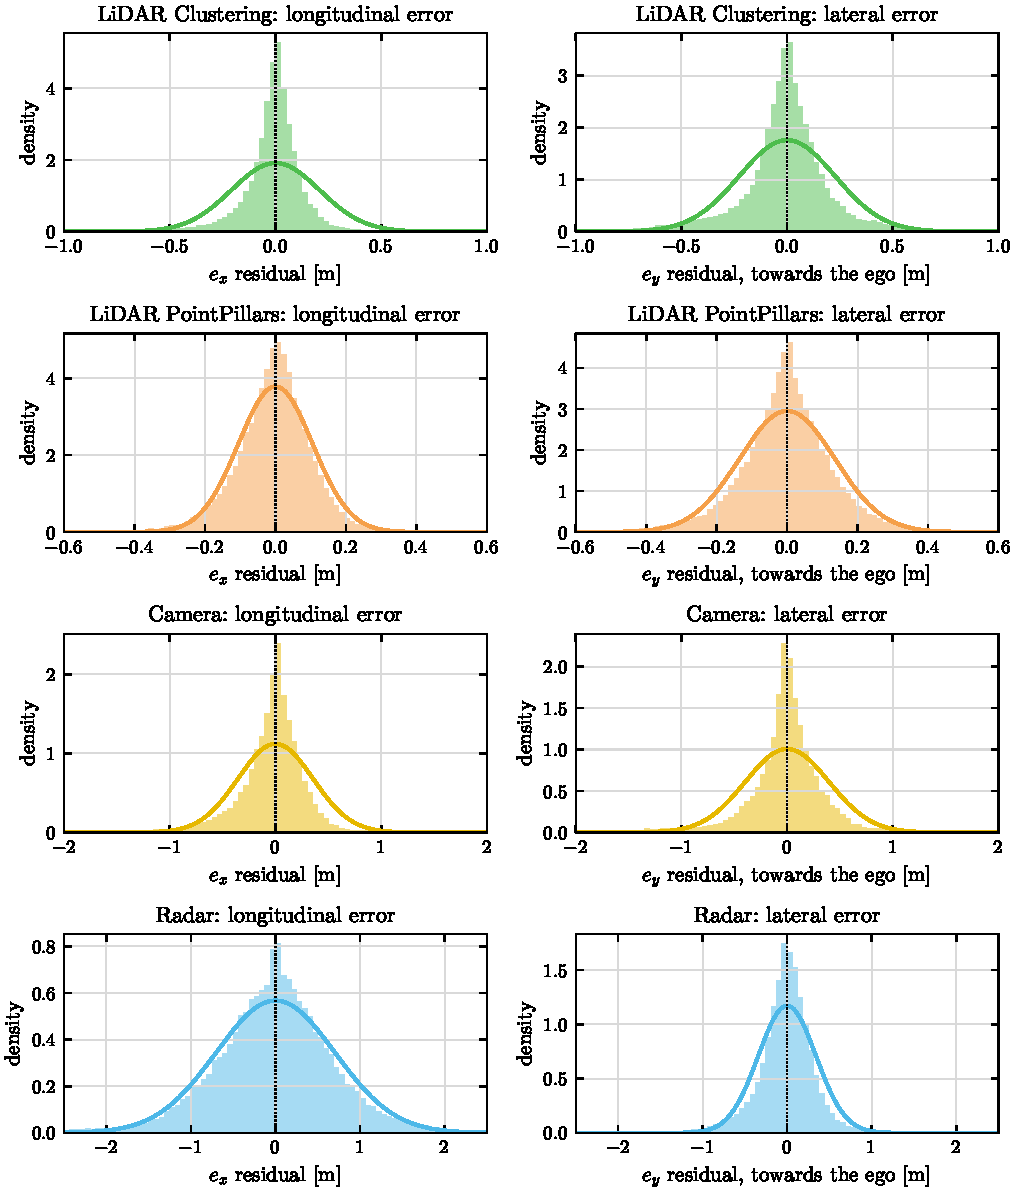
\includegraphics[width=\textwidth]{figures/ch4/gauss_std_all_sessions.pdf}
    \caption{Distributions of the residual errors of all the sessions and fitted Gaussian
    distributions.}
    \label{fig:gauss_all}
\end{figure}


%-------------------------------------------------------------------------
%	LISTS OF FIGURES AND TABLES
%-------------------------------------------------------------------------
\cleardoublepage
\addtocontents{toc}{\vspace{2em}}
\listoffigures
\listoftables

% ACKNOWLEDGEMENTS
\chapter*{Acknowledgements}
\TODO{}

\cleardoublepage

\end{document}
